%%%%%%%%%%%%%%%%%%%%%%%%%%%%%%%%%%%%%%%%%%%%%%%%%%%%%%%%%%%%%%%%%%%%%%%%%%%%%%%%
%%
%%   BornAgain Physics Manual
%%
%%   homepage:   http://www.bornagainproject.org
%%
%%   copyright:  Forschungszentrum Jülich GmbH 2015
%%
%%   license:    Creative Commons CC-BY-SA
%%
%%   authors:    Scientific Computing Group at MLZ Garching
%%               C. Durniak, M. Ganeva, G. Pospelov, W. Van Herck, J. Wuttke
%%
%%%%%%%%%%%%%%%%%%%%%%%%%%%%%%%%%%%%%%%%%%%%%%%%%%%%%%%%%%%%%%%%%%%%%%%%%%%%%%%%

% To compile this report, run
%   export T=PhysicsManual
%   xelatex $T
%   bibtex  $T
%   xelatex $T
%   makeindex $T
%   makeindex -s nomencl.ist $T.nlo -o $T.nls
%   xelatex $T

\documentclass[a4paper,11pt,fleqn]{report}\usepackage[final]{graphicx}
%\documentclass[a4paper,11pt,fleqn,draft]{report}\usepackage[final]{graphicx}
%\documentclass[a4paper,11pt,fleqn,draft]{report}\usepackage[draft]{graphicx}

\def\authors{Gennady Pospelov, Walter Van Herck, Joachim Wuttke}
\def\version{1.16}

%%%%%%%%%%%%%%%%%%%%%%%%%%%%%%%%%%%%%%%%%%%%%%%%%%%%%%%%%%%%%%%%%%%%%%%%%%%%%%%%
%%
%%   BornAgain User Manual
%%
%%   homepage:   http://www.bornagainproject.org
%%
%%   copyright:  Forschungszentrum Jülich GmbH 2015
%%
%%   license:    Creative Commons CC-BY-SA
%%   
%%   authors:    Scientific Computing Group at MLZ Garching
%%               C. Durniak, M. Ganeva, G. Pospelov, W. Van Herck, J. Wuttke
%%
%%%%%%%%%%%%%%%%%%%%%%%%%%%%%%%%%%%%%%%%%%%%%%%%%%%%%%%%%%%%%%%%%%%%%%%%%%%%%%%%

%-------------------------------------------------------------------------------
%  Page layout
%-------------------------------------------------------------------------------

\def\myparindent{5ex}
\setlength{\parindent}{\myparindent} % workaround, for colorboxes

\textwidth=410pt
\hoffset=210mm % width of A4
\advance\hoffset by -1\textwidth
\hoffset=0.5\hoffset
\advance\hoffset by -1in
% Now a slight assymmetry to leave more blank on the side of the fold
\evensidemargin=0pt
\oddsidemargin=5pt
\advance\evensidemargin by -1\oddsidemargin

\setlength{\headheight}{15pt}
\setlength{\textheight}{592pt} % default=592pt
\setlength{\marginparwidth}{7em}

\renewcommand{\arraystretch}{1.3}

%-------------------------------------------------------------------------------
%  Fancy page header
%-------------------------------------------------------------------------------

\usepackage{fancyhdr}
\pagestyle{fancy}
\fancyhf{}

\renewcommand{\sectionmark}[1]{\markright{#1}}

\fancyhead[LO,RE]{Page \thepage}
\fancyhead[LE]{\nouppercase{\leftmark}}
\fancyhead[RO]{\nouppercase{\rightmark}}


\headwidth=1.1\textwidth
\renewcommand{\headrulewidth}{1pt}%{1.5pt}
\renewcommand{\footrulewidth}{0pt}%{1.5pt}
\fancyhfoffset[L]{24pt}
\fancyhfoffset[R]{24pt}

\fancypagestyle{plain}{%
\fancyhf{} % clear all header and footer fields
\headwidth=1.1\textwidth
\renewcommand{\headrulewidth}{1pt}%{1.5pt}
\renewcommand{\footrulewidth}{0pt}
\fancyhead[LO,RE]{Page \thepage}
\fancyhead[LE]{\nouppercase{\leftmark}}
\fancyhead[RO]{\nouppercase{\rightmark}}

\fancyhfoffset[L]{24pt}
\fancyhfoffset[R]{24pt}
}

%-------------------------------------------------------------------------------
%  Symbols, fonts
%-------------------------------------------------------------------------------


\usepackage{amsmath}
\usepackage{mathtools} % has \coloneqq for :=
\usepackage{manfnt} % for \dbend
\usepackage{dingbat}

\usepackage[bold-style=ISO]{unicode-math} % must come after ams and symbols

%-------------------------------------------------------------------------------
%  Sectioning
%-------------------------------------------------------------------------------

% Add rubber to white space around chapter header
\makeatletter
\def\@makechapterhead#1{%
  \vspace*{50\p@ plus 5\p@ minus 5\p@}%
  {\parindent \z@ \raggedright \normalfont
    \ifnum \c@secnumdepth >\m@ne
        \huge\bfseries \@chapapp\space \thechapter
        \par\nobreak
        \vskip 20\p@ plus 2\p@ minus 2\p@
    \fi
    \interlinepenalty\@M
    \Huge \bfseries #1\par\nobreak
    \vskip 40\p@ plus 5\p@ minus 5\p@
  }}
\def\@makeschapterhead#1{%
  \vspace*{50\p@ plus 5\p@ minus 5\p@}%
  {\parindent \z@ \raggedright
    \normalfont
    \interlinepenalty\@M
    \Huge \bfseries  #1\par\nobreak
    \vskip 40\p@ plus 5\p@ minus 5\p@
  }}
\makeatother

\setcounter{secnumdepth}{3}
\setcounter{tocdepth}{3}
%\usepackage[toc,page]{appendix}
\usepackage{titlesec}

\newcommand{\mysection}[2]{%
                         \sectionmark{#1}%
                         \section{#2}%
                         \sectionmark{#1}%
                       }

\newcommand{\mychapter}[2]{
    \setcounter{chapter}{#1}
    \setcounter{section}{0}
    \chapter*{#2}
    \addcontentsline{toc}{chapter}{#2}
}

%-------------------------------------------------------------------------------
%  Index, List of Symbols
%-------------------------------------------------------------------------------

\usepackage{imakeidx}\makeindex
\usepackage[refpage]{nomencl}\makenomenclature
  \renewcommand{\nomname}{List of Symbols}
  % see nomencl.txt for how to force the ordering of symbols
  \def\pagedeclaration#1{, \hyperpage{#1}}%
  
\def\otherchapter#1{
  \clearpage
  \phantomsection
  \addcontentsline{toc}{chapter}{#1}
  \markboth{#1}{#1}}

%-------------------------------------------------------------------------------
%  Floats
%-------------------------------------------------------------------------------

\usepackage{subfigure}

\usepackage{placeins} % defines \FloatBarrier
\usepackage{float}
\usepackage[font={small}]{caption}

%-------------------------------------------------------------------------------
%  Tables, code listings, ...
%-------------------------------------------------------------------------------

%\usepackage{longtable}
%\usepackage{booktabs} % defines \toprule &c for use in tabular
% see http://tex.stackexchange.com/questions/78075/multi-page-with-tabulary
\usepackage{tabulary}

\usepackage[final]{listings}
\usepackage{lstcustom}
\usepackage{enumerate}
\renewcommand{\lstfontfamily}{\ttfamily}

%-------------------------------------------------------------------------------
%  Tikz pictures
%-------------------------------------------------------------------------------

\usepackage{tikz}
\usepackage{tikz-uml} 
\usetikzlibrary{trees,matrix,positioning,decorations.pathreplacing,calc}

\newcommand{\ntikzmark}[2]
           {#2\thinspace\tikz[overlay,remember picture,baseline=(#1.base)]
             {\node[inner sep=0pt] (#1) {};}}

\newcommand{\makebrace}[3]{%
    \begin{tikzpicture}[overlay, remember picture]
        \draw [decoration={brace,amplitude=0.6em},decorate]
        let \p1=(#1), \p2=(#2) in
        ({max(\x1,\x2)}, {\y1+1.5em}) -- node[right=0.6em] {#3} ({max(\x1,\x2)}, {\y2});
    \end{tikzpicture}
}

%-------------------------------------------------------------------------------
%  Highlighting
%-------------------------------------------------------------------------------

\usepackage{ifdraft}
\usepackage{mdframed}
% \usepackage{pifont}

\def\defineBox#1#2#3#4#5{
  \newmdenv[
    usetwoside=false,
    skipabove=2pt,
    skipbelow=2pt,
    leftmargin=-4pt,
    rightmargin=-4pt,
    innerleftmargin=2pt,
    innerrightmargin=2pt,
    innertopmargin=4pt,
    innerbottommargin=4pt,
    backgroundcolor=#3,
    topline=false,
    bottomline=false,
    linecolor=#4,
    linewidth=2pt,
    ]{#2*}
  \newenvironment{#1}
    {\begin{#2*}\makebox[0pt][r]{\smash{#5}}\ignorespaces}
    {\end{#2*}}
}

\def\marginSymbolLarge#1{\ifdraft{}{\raisebox{-3ex}%
{\includegraphics[width=3em]{#1}\hspace{10pt}}}}

\defineBox{boxWork}{boxxWork}{magenta!40}{magenta}
  {\marginSymbolLarge{fig/fancymanual/Arbeiten.png}}
\defineBox{boxWarn}{boxxWarn}{magenta!40}{magenta}
  {\marginSymbolLarge{fig/fancymanual/Achtung.png}}
\defineBox{boxNote}{boxxNote}{yellow!33}{yellow}{{}}
\defineBox{boxEmph}{boxxEmph}{green!20}{green}{{}}

\def\Warn#1{\begin{boxWarn}#1\end{boxWarn}}
\def\Work#1{\begin{boxWork}#1\end{boxWork}}
\def\Note#1{\begin{boxNote}#1\end{boxNote}}
\def\Emph#1{\begin{boxEmph}#1\end{boxEmph}}

\def\MissingSection{\begin{boxWork}\ldots\ to be written \ldots\end{boxWork}}

% OLD STYLE:
  
\newcommand{\BareRemark}[1]%
{\noindent\smallpencil\colorbox{blue!10}%
{\parbox{\dimexpr\linewidth-8\fboxsep}{#1}}}

\newcommand{\MakeRemark}[2]{\BareRemark{\underline{#1} #2 }}

\newcommand{\ImportantPoint}[2]
{\noindent
  {\huge\danger}\colorbox{magenta!40}{\parbox{\dimexpr\linewidth-8\fboxsep}
 {\underline{#1} #2}}}


%-------------------------------------------------------------------------------
%  Hyperref
%-------------------------------------------------------------------------------

\usepackage{hyperref} % wants to be included last
\hypersetup{
    colorlinks,
    linkcolor={red!50!black},
    citecolor={blue!50!black},
    urlcolor={blue!80!black},
    pdftitle={BornAgain User Manual} % seems to be ignored
}
\usepackage[right]{showlabels}


\begin{document}
\ifdraft{\pagenumbering{roman}}{}
\flushbottom

%%%%%%%%%%%%%%%%%%%%%%%%%%%%%%%%%%%%%%%%%%%%%%%%%%%%%%%%%%%%%%%%%%%%%%%%%%%%%%%%
%%
%%   BornAgain User Manual
%%
%%   homepage:   http://www.bornagainproject.org
%%
%%   copyright:  Forschungszentrum Jülich GmbH 2015
%%
%%   license:    Creative Commons CC-BY-SA
%%   
%%   authors:    Scientific Computing Group at MLZ Garching
%%               C. Durniak, M. Ganeva, G. Pospelov, W. Van Herck, J. Wuttke
%%
%%%%%%%%%%%%%%%%%%%%%%%%%%%%%%%%%%%%%%%%%%%%%%%%%%%%%%%%%%%%%%%%%%%%%%%%%%%%%%%%

% Math operators (AtBeginDocument to prevent unicode-math from overwriting)
\AtBeginDocument{\renewcommand{\Re}{\operatorname{Re}}}
\AtBeginDocument{\renewcommand{\Im}{\operatorname{Im}}}

\DeclareMathOperator{\sinc}{sinc}

% Vectors
\renewcommand{\v}[1]{\ensuremath{\mathbf{#1}}}
\newcommand{\unitvec}[1]{\ensuremath{\widehat{\vect{#1}}}}
\newcommand{\Nabla}{\mathbf{\nabla}}

% Curly letters
\newcommand{\curlf}{\ensuremath{\mathcal{F}}}
\newcommand{\curlp}{\ensuremath{\mathcal{P}}}
\def\Sample{\ensuremath{\mathcal{M}}}
\def\Sphere{\ensuremath{\mathcal{S}}}

% Ensemble average
\newcommand{\bra}{\ensuremath{\left\langle}}
\newcommand{\ket}{\ensuremath{\right\rangle}}

% Pair correlation functions
\newcommand{\ppcf}[3]{\ensuremath{\mathcal{G}_{#1 ,#2}\left( \v{#3}_{#1} , \v{#3}_{#2} \right)}}
\newcommand{\ppcfb}[3]{\ensuremath{\mathcal{G}_{#1 #2}\left( \v{#3}_{#1 #2} \right)}}

% Fixed-font words
\newcommand{\Code}[1]{\texttt{#1}}
\newcommand{\BornAgain}{\Code{Born\discretionary{}{}{}Again}}%
\newcommand{\Python}{\Code{Python}}%
\newcommand{\IsGISAXS}{\Code{IsGISAXS}}%


\def\d{\text{d}}
\def\e{\text{e}}
\def\E#1{\textsl{#1}}
\def\etal{\E{et al.}}
\def\FD{\mathcal{F}}
\def\GD{\mathcal{G}}
\def\idest{\E{i.e.\ }}
\def\il{l} % index for layer
\def\k{\v{k}}
\def\kD{\k_\text{D}}
\def\nz{\overline{n^2}}
\def\nzj{\overline{n_\il^2}}
\def\plll{\parallel}
\def\PD{\mathcal{P}}
\def\q{\v{q}}
\def\r{\v{r}}
\def\R{\v{R}}
\def\rD{\r_\text{D}}
\def\rS{\r_\text{S}}
\def\ti{\text{i}}
\def\tf{\text{f}}

\renewcommand{\u}[1]{\underline{#1}}
\newcommand{\uu}[1]{\underline{\underline{#1}}}
\newcommand{\UP}{\uparrow}
\newcommand{\DN}{\downarrow}


%-------------------------------------------------------------------------------
%	HYPHENATION
%-------------------------------------------------------------------------------

\hyphenation{ MacOS Schrö-ding-er nano-par-ti-cle nano-par-ti-cles }

%%%%%%%%%%%%%%%%%%%%%%%%%%%%%%%%%%%%%%%%%%%%%%%%%%%%%%%%%%%%%%%%%%%%%%%%%%%%%%%%
%%
%%   BornAgain User Manual
%%
%%   homepage:   http://www.bornagainproject.org
%%
%%   copyright:  Forschungszentrum Jülich GmbH 2015
%%
%%   license:    Creative Commons CC-BY-SA
%%
%%   authors:    Scientific Computing Group at MLZ Garching
%%               C. Durniak, M. Ganeva, G. Pospelov, W. Van Herck, J. Wuttke
%%
%%%%%%%%%%%%%%%%%%%%%%%%%%%%%%%%%%%%%%%%%%%%%%%%%%%%%%%%%%%%%%%%%%%%%%%%%%%%%%%%

%-------------------------------------------------------------------------------
%  Title page
%-------------------------------------------------------------------------------

\thispagestyle{empty}
\strut\vspace{10mm}
\begin{center}
\Huge
{\bf BornAgain}\\[10mm]
\Large
Software for simulating and fitting\\[.2ex]
X-ray and neutron small-angle scattering\\[.2ex]
at grazing incidence\\[15mm]
User Manual\\[5mm]
\large
Version \version (\today)\\[30mm]
\Large
\authors\\[10mm]
\large
Scientific Computing Group\\[.2ex]
J\"ulich Centre for Neutron Science\\[.2ex]
at Heinz Maier-Leibnitz Zentrum Garching\\[.2ex]
Forschungszentrum J\"ulich GmbH
\end{center}
\newpage

%------------------------------------------------------------------------------
%	DOCUMENT
%------------------------------------------------------------------------------


% Back of title page.
\thispagestyle{empty}
~\vfill
\noindent
\begin{tabular}{@{}p{.25\textwidth}@{}p{.75\textwidth}@{}}
Homepage:  &\url{http://www.bornagainproject.org}\\[2ex]
Copyright:  &Forschungszentrum Jülich GmbH 2013--\the\year\\[2ex]
Licenses:   &Software: GNU General Public License version 3 or higher\\
            &Documentation: Creative Commons CC-BY-SA\\[2ex]
Authors:    &\authors\\
            &Scientific Computing Group\\
            &at Heinz Maier-Leibnitz Zentrum (MLZ) Garching\\[2ex]
Disclaimer: &Software and documentation are work in progress.\\
            &We cannot guarantee correctness and accuracy.\\
            &If in doubt, contact us for assistance or scientific collaboration.\\[2ex]
Funding:    &This project has received funding from the European Union’s
             Horizon 2020 research and innovation programme under grant agreement No 654000.
\end{tabular}
\newpage


\tableofcontents\cleardoublepage

%%%%%%%%%%%%%%%%%%%%%%%%%%%%%%%%%%%%%%%%%%%%%%%%%%%%%%%%%%%%%%%%%%%%%%%%%%%%%%%%
%%
%%   BornAgain User Manual
%%
%%   homepage:   http://www.bornagainproject.org
%%
%%   copyright:  Forschungszentrum Jülich GmbH 2015
%%
%%   license:    Creative Commons CC-BY-SA
%%
%%   authors:    Scientific Computing Group at MLZ Garching
%%               C. Durniak, M. Ganeva, G. Pospelov, W. Van Herck, J. Wuttke
%%
%%%%%%%%%%%%%%%%%%%%%%%%%%%%%%%%%%%%%%%%%%%%%%%%%%%%%%%%%%%%%%%%%%%%%%%%%%%%%%%%


\cleardoublepage
\ichapter{Preface}

%%%%%%%%%%%%%%%%%%%%%%%%%%%%%%%%%%%%%%%%%%%%%%%%%%%%%%%%%%%%%%%%%%%%%%%%%%%%%%%%
\isection{About BornAgain}
%%%%%%%%%%%%%%%%%%%%%%%%%%%%%%%%%%%%%%%%%%%%%%%%%%%%%%%%%%%%%%%%%%%%%%%%%%%%%%%%

BornAgain is a software package
to simulate and fit
reflectometry, off-specular scattering,
and grazing-incidence small-angle scattering (GISAS)
of X-rays and neutrons.
It provides a generic framework
for modeling multilayer samples with smooth or
rough interfaces and with various types of embedded nanoparticles.
The name, \BornAgain,
alludes to the central role of the distorted-wave Born
approximation (DWBA) in the physical description of the
scattering process.
\index{Distorted-wave Born approximation}

BornAgain is maintained
by the Scientific Computing Group
of the J\"ulich Centre for Neutron Science (JCNS)
at Heinz Maier-Leibnitz Zentrum (MLZ) Garching, Germany.
It free and open source software.
The source code is released under the GNU General Public License (GPL, version 3 or higher),
the documentation under the Creative Commons license CC-BY-SA.

%%%%%%%%%%%%%%%%%%%%%%%%%%%%%%%%%%%%%%%%%%%%%%%%%%%%%%%%%%%%%%%%%%%%%%%%%%%%%%%%
\isection{Citation}
%%%%%%%%%%%%%%%%%%%%%%%%%%%%%%%%%%%%%%%%%%%%%%%%%%%%%%%%%%%%%%%%%%%%%%%%%%%%%%%%

The canonical reference for BornAgain is the journal article
\begin{quote}
Gennady Pospelov, Walter Van Herck, Jan Burle, Juan M. Carmona Loaiza,
Céline Durniak, Jonathan M. Fisher, Marina Ganeva, Dmitry Yurov and
Joachim Wuttke:\\
BornAgain : software for simulating and fitting
grazing-incidence small-angle scattering\\
\href{https://doi.org/10.1107/S1600576719016789}{J. Appl. Cryst. 53, 262–276 (2020)}
\end{quote}
Use of the software version should additionally be documented by citing a specific version
\index{Citation}%
\begin{quote}
BornAgain --- Software for simulating and fitting
X-ray and neutron small-angle scattering at grazing incidence,
version $\langle$\texttt{version}$\rangle$ ($\langle$\texttt{release date}$\rangle$),\\
\url{http://www.bornagainproject.org}
\end{quote}
Citation of the present document is only necessary
when referring to specific information about form factors.

\pagemode{\thechapter}

%%%%%%%%%%%%%%%%%%%%%%%%%%%%%%%%%%%%%%%%%%%%%%%%%%%%%%%%%%%%%%%%%%%%%%%%%%%%%%%%
%%
%%   BornAgain User Manual
%%
%%   homepage:   http://www.bornagainproject.org
%%
%%   copyright:  Forschungszentrum Jülich GmbH 2015
%%
%%   license:    Creative Commons CC-BY-SA
%%
%%   authors:    Scientific Computing Group at MLZ Garching
%%               C. Durniak, M. Ganeva, G. Pospelov, W. Van Herck, J. Wuttke
%%
%%%%%%%%%%%%%%%%%%%%%%%%%%%%%%%%%%%%%%%%%%%%%%%%%%%%%%%%%%%%%%%%%%%%%%%%%%%%%%%%

\def\Do{\overset{o}{D}}
\def\Go{\overset{o}{G}}
\def\TD{\TENS{D}}
\def\TG{\TENS{G}}
\def\TDo{\TENS{\overset{o}{D}}}
\def\TGo{\TENS{\overset{o}{G}}}
\def\Psio{\TENS{\overset{o}{\Psi}}}

\def\pfo{\overset{o}{\psi}_\sf}
\def\pfoc{\overset{o}{\psi}\vphantom{\psi}^*_\sf}

\index{Scattering!target|see{Sample}}%
\index{Elastic scattering|seealso{Cross section}}%

\part{Physics}\label{PPHYS}

\chapter{Scattering}  \label{SSca}
\chaptermark{Scattering}

TODO: REWRITE
This chapter introduces the basic theory of small-angle scattering (SAS).
\index{Small-angle scattering}%
\index{SAS|see{Small-angle scattering}}%
We specifically consider scalar neutron and X-ray propagation,
adjourning the notationally more involved
theory of polarized neutrons to \Cref{SPol}.
Our exposition is self-contained,
except for the initial passage from the microscopic
to the macroscopic Schrödinger equation,
which we outline only briefly (\Cref{Swave}).
For X-rays, we obtain the same perturbed Schrödinger equation from Maxwell's equations
(\Cref{SXray}).
The standard description of scattering in first-order Born approximation
(\Cref{SBornApprox})
is introduced in a way that facilitates the following generalization
into the distorted-wave Born approximation (DWBA)
needed for grazing-incidence scattering (\Cref{SDWBA}).
This chapter finishes with a qualitative discussion
of coherence lengths (\Cref{Scoherlen}).

%%%%%%%%%%%%%%%%%%%%%%%%%%%%%%%%%%%%%%%%%%%%%%%%%%%%%%%%%%%%%%%%%%%%%%%%%%%%%%%%
\section{Wave propagation}\label{Swave}
%%%%%%%%%%%%%%%%%%%%%%%%%%%%%%%%%%%%%%%%%%%%%%%%%%%%%%%%%%%%%%%%%%%%%%%%%%%%%%%%
\index{Wave propagation|(}%

%===============================================================================
\subsection{Coherent neutron wave}\label{ScohWave}
%===============================================================================
\index{Wave propagation!neutron|(}%
\index{Neutron!wave propagation|(}%

\def\Vmac{\tilde{V}}

\index{Schrodinger@Schrödinger equation!microscopic}%
The scalar wavefunction $\psi(\r,t)$
\nomenclature[2t020]{$t$}{Time}%
\nomenclature[2r040]{$\r$}{Position}%
\nomenclature[1ψ030 2r040 2t02]{$\psi(\r,t)$}{Microscopic neutron wavefunction}%
of a free neutron
in absence of a magnetic field
is governed by the Schrödinger equation
\begin{equation}\label{ESchrodi}
  i\hbar\partial_t \psi(\r,t)
  = \left\{-\frac{\hbar^2}{2m}\Nabla^2+V(\r)\right\} \psi(\r,t).
\end{equation}
Since BornAgain only aims at modelling elastic scattering,
\index{Scattering!elastic}%
any time dependence of the potential is averaged out in the definition
\index{Potential!neutron}%
\index{Neutron!potential}%
$V(\r)\coloneqq \langle V(\r,t)\rangle$.
\nomenclature[2v130 2r040]{$V(\r)$}{Neutron potential}%
\index{Time dependence!neutron potential}%
Inelastic scattering,
\index{Inelastic scattering}%
\index{Scattering!inelastic}%
\index{Damping!inelastic scattering}%
\index{Loss terms|see {Damping}}%
in principle, can be accounted for by an extra contribution
damping.\footnote
{This is not explicitly supported in the software,
but users are free to increase the imaginary part of the refractive index
\index{Refractive index!emulate inelastic scattering}%
to emulate damping by inelastic losses.}
Therefore we only need to consider monochromatic waves
\index{Wave!monochromatic}%
\index{Monochromatic wave}%
with given frequency~$\omega$.
\nomenclature[1ω 020]{$\omega$}{Frequency of incident radiation}%
In consequence, the wavefunction
\begin{equation}\label{Estationarywave}
  \psi(\r,t) = \psi(\r)\e^{-i\omega t}
\end{equation}
\nomenclature[1ψ030 2r040 0]{$\psi(\r)$}{Stationary wavefunction}%
factorizes into a stationary wave and a time-dependent phase factor.%
\index{Stationary wavefunction}%
\index{Phase factor}%
Inserting \cref{Estationarywave} in \cref{ESchrodi},
we obtain the stationary Schrödinger equation
\begin{equation}\label{EstatSchrodi}
  \left\{-\frac{\hbar^2}{2m}\Nabla^2+V(\r)-\hbar\omega\right\} \psi(\r) = 0.
\end{equation}
\nomenclature[2m020]{$m$}{Neutron mass}%
\index{Potential|see {Optical potential}}%
\index{Optical potential!nuclear (microscopic)}%
The \E{nuclear} (or \E{microscopic})
\E{optical potential} $V(\r)$,
in a somewhat ``naive conception'' \cite[p.~7]{Sea89},
consists of a sum of delta functions,
representing Fermi's ``pseudopotential''.
\index{Fermi's pseudopotential}%
The superposition of the incident wave with the scattered waves
\index{Scattering!coherent forward}%
originating from each illuminated nucleus
results in \E{coherent forward scattering},
\index{Coherent forward scattering}%
in line with Huygens' principle.
\index{Huygens' principle}%

Coherent superposition also leads to \E{Bragg scattering}.
\index{Bragg scattering!by atomic lattices}%
However, Bragg scattering by atomic lattices only occurs at angles
far above the small-angle range covered in GISAS experiments.
Accordingly, it can be neglected in the analysis of GISAS data,
or at most, is taken into account as a loss channel.

Therefore,
we can neglect the atomic structure of $V(\r)$,
and perform some coarse graining to
arrive at a \E{continuum approximation}.
\index{Continuum approximation!neutron propagation}%
This is
similar to the passage from
the microscopic to the macroscopic Maxwell equations.
The details are intricate \cite{Sea89,Lax51},
but the result \cite[eq.~2.8.32]{Sea89} is very simple:
The macroscopic field equation
has still the form of a stationary Schrödinger equation,
\index{Schrodinger@Schrödinger equation!macroscopic}%
\begin{equation}\label{EmacrSchrodi}
  \left\{-\frac{\hbar^2}{2m}\Nabla^2+\Vmac(\r)-\hbar\omega\right\} \psi(\r) = 0,
\end{equation}
\nomenclature[1ψ030 2r040]{$\psi(\r)$}{Stationary coherent wavefunction}%
where $\psi$ now stands for the \E{coherent wavefunction}
\index{Coherent wavefunction}%
\index{Wave propagation!coherent}%
obtained by superposition of incident and forward scattered states.
The \E{macroscopic optical potential}.
\nomenclature[2v131 2r040]{$\Vmac(\r)$}{Macroscopic optical potential}%
\index{Optical potential!macroscopic}%
\begin{equation}
  \Vmac(\r) = \frac{2\pi\hbar^2}{m}\left\langle b(\r) \right\rangle
\end{equation}
depends on the \E{bound scattering length density}
\begin{equation}
  b(\r) = \sum_j b_j\delta(\r-\r_j).
\end{equation}
The \E{bound scattering length} $b_j$ is isotope specific;
values are tabulated \cite{Sea92}.
For a monatomic system
(with no correlation between nuclear spin or isotopic composition and position),
\begin{equation}
  \left\langle b(\r) \right\rangle = b_\text{c} \left\langle\rho(\r)\right\rangle
\end{equation}
with the \E{bound coherent scattering length} $b_\text{c}$ and the number density~$\rho(\r)$.

The macroscopic optical potential is weak, and slowly varying compared to atomic length scales.
In the following it shall be expressed through the
\E{bound scattering length density} (SLD)
\index{Bound scattering length|see{Scattering length}}%
\index{Scattering!length density}%
\index{SLD|see{Scattering length density}}%
\cite[eq.\ 2.8.37]{Sea89},
\nomenclature[2v030 2r040]{$v(\r)$}{Scattering length density (SLD)}%
\begin{equation}\label{Edefv}
  v(\r)
  \coloneqq\frac{m}{2\pi \hbar^2}\Vmac(\r)
  = \left\langle b(\r) \right\rangle
\end{equation}
In the following, we will characterize the incoming radiation
not by its energy~$\hbar\omega$,
but by its \E{vacuum wavenumber}~$K$,
\index{Vacuum!neutron wavenumber}%
\index{Wavenumber!neutron}%
\nomenclature[2k120]{$K$}{Wavenumber in vacuum}%
given by the dispersion relation
\index{Dispersion relation!neutron}%
\index{Neutron!dispersion relation}%
\begin{equation}
  \hbar\omega = \frac{(\hbar K)^2}{2m}.
\end{equation}
The macroscopic Schrödinger equation~\cref{EmacrSchrodi} then takes the simple form
\Emph{
\begin{equation}\label{ESchrodi2}
  \left\{\Nabla^2+K^2-4\pi v(\r)\right\} \psi(\r) = 0.
\end{equation}
\vspace*{-5pt}}
In neutron optical applications, like wave propagation through multilayers,
it is convenient to parametrize $\mv(\r)$ in terms of the \E{refractive index}
\begin{equation}\label{EnkK}
  n(\r)\coloneqq\sqrt{1-\frac{4\pi\mv(\r)}{K^2}}.
\end{equation}
\nomenclature[2n020]{$n$}{Refractive index}%
\index{Refractive index!neutron}%
\index{Index of refraction|see {Refractive index}}%
If $\mv(\r)$ has an imaginary part, describing absorption,
\index{Absorption}%
then $n(\r)$ is a complex number.
Conventionally, $n$ is parameterized by two real numbers:
\begin{equation}\label{Endb1}
  n \eqqcolon  1-\delta +i\beta.
\end{equation}
\nomenclature[1δ020]{$\delta$}{Small parameter in the refractive index
   $n=1-\delta +i\beta$}%
\nomenclature[1β020]{$\beta$}{Imaginary part of the refractive index}%
For thermal neutrons,
$\delta$ and $\beta$ are almost always nonnegative,\footnote
{The plus sign in front of~$i\beta$ is a consequence of
the quantum-mechanical sign convention;
in the X-ray crystallography convention it would be a minus sign.
\index{Refractive index!sign convention}%
\index{Sign convention!refractive index}}
and much smaller than~1.

%===============================================================================
\subsection{Neutrons in a magnetic field}\label{Snpwave}
%===============================================================================

\index{Neutron!spin|(}%
\index{Spin|(}%
\index{Magnetic field!neutron propagation|(}%

\index{Field!magnetic|see{Magnetic field}}%
\index{H Field@$H$ Field|see{Magnetizing field}}%
\index{B Field@$H$ Field|see{Magnetizing field}}%

In presence of a magnetic field,
the propagation of free neutrons becomes spin dependent.
Therefore the scalar wavefunction of \cref{ScohWave}
must be replaced by spinor $\v\Psi$.
\index{Spinor}%
The magnetic moment of the neutron couples to the magnetizing field~$\v{H}$ \cite{Mez86}.
\nomenclature[2h150 2r040 2t020]{$\v{H}(\r,t)$}{Magnetizing field}%
\index{Magnetizing field!coupling to neutron moment}%
With the coupling term, the macroscopic Schrödinger equation~\cref{EmacrSchrodi}
\index{Schrodinger@Schrödinger equation!macroscopic}%
becomes
\begin{equation}\label{EHSchrodi}
  \left\{-\frac{\hbar^2}{2m}\Nabla^2+\Vmac(\r)
         +\mu_0\mu_\text{n}\v{H}(\r)\v{\sigma}-\hbar\omega\right\}
      \v\Psi(\r) = 0,
\end{equation}
\nomenclature[1ψ150 2r040]{$\v\Psi(\r)$}{Stationary coherent spinor wavefunction}%
where $\mu_0$ is the vacuum permeability,
\nomenclature[1μ024 00]{$\mu_0$}{Vacuum permeability, $4\pi\cdot10^{-7}$ Vs/Am}%
\index{Permeability}%
\index{Magnetic permeability}%
$\mu_\text{n}$ is the magnetic moment of the neutron,
\nomenclature[1μ024 2n000]{$\mu_\text{n}$}{Magnetic moment of the neutron}
\index{Neutron!magnetic moment}%
\index{Magnetic moment!neutron}%
and ${\v\sigma}$ is the Pauli vector, composed of the three Pauli matrices.
\nomenclature[1σ04]{$\v\sigma$}{Pauli
    vector, composed of the three Pauli matrices: $\v\sigma=(\sigma_x,\sigma_y,\sigma_z)$}%
\index{Pauli vector}%
\index{Pauli matrix}%
The magnetic coupling is responsible for Larmor precession of the neutron spin,
\index{Neutron!Larmor precession}%
\index{Larmor precession}%
\index{Spin!Larmor precession}%
well known from uses in spin-echo techniques.
\index{Spin!echo}%
If the field is inhomogeneous,
it can split a beam
as in the Stern-Gerlach experiment \cite{ShSB54}.
\index{Neutron!Stern-Gerlach splitting}%
\index{Stern-Gerlach splitting}%

We introduce the reduced field
\begin{equation}
  \v{h} \coloneqq \frac{m\mu_0\mu_\text{n}}{2\pi\hbar^2}\v{H},
\end{equation}
\nomenclature[2h050 2r040]{$\v{h}(\r)$}{Rescaled
   field $\v{h}=(m\mu_0\mu_\text{n}/2\pi\hbar^2)\v{H}$}%
\index{Magnetizing field!reduced}%
to rewrite the macroscopic Schrödinger equation in analogy to~\cref{ESchrodi2} as
\index{Schrodinger@Schrödinger equation!macroscopic}%
\Emph{
\begin{equation}\label{ESchrodi2H}
  \left\{\Nabla^2+K^2-4\pi v(\r)-\v{h}(\r)\v{\sigma}\right\} \v\Psi(\r) = 0.
\end{equation}
\vspace*{-5pt}}


\index{Spin|(}%
\index{Neutron!spin|)}%
\index{Magnetic field!neutron propagation|)}%

\index{Wave propagation!neutron|)}%
\index{Neutron!wave propagation|)}%

%===============================================================================
\subsection{X-ray propagation}\label{SXwave}
%===============================================================================

\index{Wave propagation!X-ray|(}%

The propagation of X-rays is governed by Maxwell's equations,
\index{Maxwell's equations}%
\begin{equation}\label{EMaxwell}
  \begin{array}{@{}l@{\quad}l@{\quad}l}
    \Nabla\times\v{E}=-\partial_t \v{B},
   &\Nabla\v{B}=0,
   &\v{B}=\v{\mu}(\r)\mu_0\v{H},
   \\[2ex]
    \Nabla\times\v{H}=+\partial_t \v{D},
   &\Nabla\v{D}=0,
   &\v{D}=\v{\eps}(\r)\eps_0\v{E}.
  \end{array}
\end{equation}
\nomenclature[2e150 2r040 2t020]{$\v{E}(\r,t)$}{Electric field}%
\nomenclature[2d150 2r040 2t020]{$\v{D}(\r,t)$}{Displacement field}%
\nomenclature[2b150 2r040 2t020]{$\v{B}(\r,t)$}{Magnetic field}%
\nomenclature[1ε070 2r040]{$\v\eps(\r)$}{Relative dielectric permittivity tensor}%
\nomenclature[1μ070 2r040]{$\v\mu(\r)$}{Relative magnetic permeability tensor}%
\nomenclature[1ε024 00]{$\eps_0$}{Vacuum permittivity, 8.854\ldots As/Vm}%
Since BornAgain only addresses elastic scattering,
\index{Elastic scattering}%
\index{Scattering!elastic}%
we assume the permeability and permittivity tensors $\v\mu$ and~$\v\eps$
to be time-independent.
\index{Time dependence!dielectric permittivity}%
Therefore, as in~\cref{ScohWave}, we only need to consider monochromatic waves
\index{Wave!monochromatic}%
\index{Monochromatic wave}%
with given frequency~$\omega$,
and each of the fields $\v{E}$, $\v{D}$, $\v{H}$, $\v{B}$
factorizes into a stationary field and a time-dependent phase factor.\footnote
{This phase factor can be defined with a plus or a minus sign in the exponent.
Most texts on X-ray crystallography,
including influential texts on GISAXS \cite{ReLL09},
prefer the \E{crystallographic convention} with a plus sign.
\index{Wave propagation|seealso {Sign convention}}%
\index{Convention!sign convention}%
\index{Sign convention!wave propagation|(}%
\index{Crystallographic sign convention}%
In BornAgain, we prefer the opposite \E{quantum-mechanical convention}
\index{Quantum-mechanical convention}%
for consistency with the neutron case \cref{Estationarywave},
where the minus sign is an inevitable consequence
of the standard form of the Schrödinger equation.%
\index{Sign convention!wave propagation|)}%
}
\index{Phase factor}%
In the following, we will concentrate on the electric field
\index{Electric field}%
\begin{equation}\label{EstationaryX}
  \v{E}(\r,t) = \v{E}(\r)\e^{-i\omega t}.
\end{equation}
The other three fields can be obtained from~$\v{E}$
by straightforward application of~\cref{EMaxwell}.

Since magnetic refraction or scattering is beyong the scope of BornAgain,
the relative magnetic permeability tensor is always $\v{\mu}(\r)=1$.
\index{Permeability}%
\index{Magnetic permeability}%
As customary in SAXS and GISAXS,
\index{Grazing-incidence small-angle scattering!dielectric model}%
\index{Small-angle scattering!dielectric model}%
we assume
that the dielectric properties of the material are those of a polarizable electron cloud.\footnote
{This is occasionally called the \E{Laue model}
\index{Laue model}%
 \cite{Lau31}.}
Thereby the relative dielectric permittivity tensor~$\v{\eps}$
\index{Dielectric permittivity}%
\index{Permittivity}%
becomes a scalar,
\begin{equation}
  \eps(\r)=1-\frac{4\pi r_e}{K^2}\rho(\r),
\end{equation}
\nomenclature[1ε030 2r040]{$\eps(\r)$}{Relative dielectric permittivity function}%
\nomenclature[1ρ030 2r040]{$\rho(\r)$}{Electron number density}%
with the classical electron radius~$r_e=e^2/mc^2\simeq2.8\cdot10^{-15}$~m,
\index{Electron radius}%
\index{Classical electron radius}%
\nomenclature[2r024 2e000]{$r_e$}{Classical electron radius~$2.817\ldots^{-15}$~m}%
the electron number density~$\rho(\r)$,
\index{Electron density}%
\index{Density!electron}%
\index{Number density|see{Density}}%
and the vacuum wavenumber~$K$,
given by the dispersion relation
\begin{equation}
  K^2 = \mu_0\eps_0\omega^2.
\end{equation}
\index{Dispersion!X-ray}%
The refractive index
\begin{equation}\label{EnX}
  n(\r)\coloneqq\sqrt{\epsilon(\r)} \eqqcolon 1-\delta+i\beta
\end{equation}
\index{Refractive index!X-rays}%
can be parametrized as in~\cref{Endb1}.
For X-rays, as for thermal neutrons, the parameters $\delta$ and~$\beta$ are nonnegative,
and much smaller than~1.

With these simplifying assumptions about $\v{\eps}$ and~$\v{\mu}$,
Maxwell's equations yield the wave equation
\begin{equation}\label{ENabCrossNabE}
  \Nabla\times\Nabla\times\v{E} = K^2\eps(\r)\v{E}.
\end{equation}
\index{Wave equation!X-ray}%
\index{X-ray!wave equation}%
Using a standard identity from vector analysis, it can be brought into the more tractable form
\Emph{
\begin{equation}\label{ENabNabE}
  \left\{\Nabla^2-\Nabla\cdot\Nabla+ K^2\eps(\r)\right\}\v{E}(\r)=0,
\end{equation}
\vspace*{-5pt}}
which closely ressembles the macroscopic Schrödinger equation~\cref{ESchrodi2},
except for the additional dyadic differential operator $\Nabla\cdot\Nabla$,
and for the transverse vector character of the electric field~$\E(\r)$.

\index{Wave propagation!X-ray|)}%

%%%%%%%%%%%%%%%%%%%%%%%%%%%%%%%%%%%%%%%%%%%%%%%%%%%%%%%%%%%%%%%%%%%%%%%%%%%%%%%%
\section{Distorted-wave Born approximation}\label{SDWBA}
%%%%%%%%%%%%%%%%%%%%%%%%%%%%%%%%%%%%%%%%%%%%%%%%%%%%%%%%%%%%%%%%%%%%%%%%%%%%%%%%

%===============================================================================
\subsection{Perturbed wave equation}\label{Sfluct}
%===============================================================================

We now begin to study scattering by condensed-matter samples
(we will prefer the brief term \E{sample} over \E{scattering target}).
\index{Sample}%
We will determine scattering cross sections
\index{Cross section}%
\index{Scattering!cross section}%
by solving the wave equations \cref{ESchrodi2,ESchrodi2H,ENabNabE}
through a perturbation expansion.
\index{Perturbation expansion}%
However, to achieve rapid convergence
we must not treat \E{all} of $v(\r)$, $\v{h}(\r)$ or $\epsilon(\r)$
as a perturbation.
Rather, we will decompose each of these fields into a more \E{regular}
and a more \E{fluctuating} part:
\begin{align}
  v(\r) &= \mv(\r) + \delta v(\r),\\
  \v{h}(\r) &= \overline{\v{h}}(\r) + \delta\v{h}(r),\\
  \epsilon(\r) &= \overline\epsilon(\r) + \delta\epsilon(\r).
\end{align}
The fluctuating parts stand for the more irregular features of a sample
one ultimately wants to study in a scattering experiment.
If they are zero,
then the remaining wave equations shall be simple enough to allow
for analytical solutions.
These solutions will be called \E{distorted waves}.
\index{Distorted wave}%
\index{Wave!distorted}%
They are distorted with respect to the plane \E{vacuum waves}
\index{Vacuum!wave}%
\index{Wave!vacuum}%
\index{Plane!wave}%
\index{Wave!plane}%
that are obtained as solution of the wave equations
for $\r$ outside the finite sample,
under the vacuum conditions $v=0$, $\v{h}=0$, $\epsilon=1$.

In the following,
we develop a generic formalism for the scattering of distorted neutron or X-ray waves.
Wave propagation in vacuum shall be denoted by an overset circle.
The wave equation in vacuum shall be written as
\Emph{
\begin{equation}\label{EDPsi0}
  \TDo\,\Psio(\r)=0.
\end{equation}
\vspace*{-5pt}}
Literally, this is an equation for the neutron spinor wavefunction.
It is, however, equally applicable for scalar neutron wavefunctions~$\psi(\r)$
or electric fields~$\v{E}(\r)$.
The differential operator in~\cref{EDPsi0} is
\begin{align}
  \Do &\coloneqq \Nabla^2 + K^2 &\text{ neutron (scalar),}\\
  \TDo &\coloneqq \Nabla^2 + K^2 &\text{ neutron (spinorial),}\\
  \TDo &\coloneqq \Nabla^2 - \Nabla\cdot\Nabla + K^2 &\text{ X-rays.}
\end{align}
\nomenclature[2d138 2r040]{$\Do(\r)$}{Differential operator in the vacuum wave equation}%
Distorted-wave propagation is described by the differential operator
\begin{equation}
  \TD(\r) \coloneqq \TDo + \TENS{\Lambda}(\r)
\end{equation}
with the distortion field
\begin{align}
  \Lambda(\r) &\coloneqq 4\pi\mv(\r)
      &\text{ neutron (scalar),}\\
  \TENS{\Lambda}(\r) &\coloneqq 4\pi\mv(\r)+\overline{\v{h}}(\r)\v\sigma
      &\text{ neutron (spinorial),}\\
  \Lambda(\r) &\coloneqq K^2(\epsilon(\r)-1)
      &\text{ X-rays.}
\end{align}
If it is scalar, then it can be expressed through the refractive index,
defined in \cref{EnkK} or~\cref{EnX}:
\index{Refractive index}%
\begin{equation}\label{EnkK}
  n(\r)\coloneqq\sqrt{1-\frac{\Lambda(\r)}{K^2}}.
\end{equation}

The full wave equation, valid inside and outside the sample,
can then be written as
\Emph{
\begin{equation}\label{EDPsi}
  \TD(\r)\v\Psi(\r) = 4\pi\TENS{U}(\r)
\end{equation}
\vspace*{-5pt}}
with
\begin{align}
  U(\r) &\coloneqq \delta v(\r)
      &\text{ neutron (scalar),}\\
  \TENS{U}(\r) &\coloneqq \delta v(\r)+\delta{\v{h}}(\r)\v\sigma/(4\pi)
      &\text{ neutron (spinorial),}\\
  U(\r) &\coloneqq K^2\delta \epsilon(\r)/(4\pi)
      &\text{ X-rays.}
\end{align}
Since the field~$U(\r)$ on the right-hand side of \cref{EDPsi}
is due to fluations of $n(\r)$,
its absolute values are always much smaller than~1.
This enables us to solve \cref{EDPsi} by a first-order perturbation theory,
\index{Perturbation expansion}%
the \E{distorted-wave Born approximation} (DWBA).
\index{Distorted-wave Born approximation}%
The DWBA generalizes the standard \E{Born approximation},
\index{Born approximation}%
which corresponds to the special case~$\v\Lambda(\r)=0$.

%===============================================================================
\subsection{Reciprocity of the Green function}\label{SReci}
%===============================================================================

\index{Reciprocity|(}%
\index{Green function!reciprocity|(}%

Our computation of~$G_\infty$ will be based on a source-detector \E{reciprocity theorem}
for the scalar Schrödinger equation.\footnote
{There exists a confusing multitude of reciprocity theorems \cite{Pot04}.
In the end, we found it simpler to provide a derivation taylored for our application case
than to refer to the literature.}
The theorem states:
Any Green function $G(\r,\r')$
that solves~\cref{EGreenK} and as function of~$\r$ represents an outgoing wave
[in accord with the Sommerfeld radiation condition,
\index{Sommerfeld radiation condition}%
\index{Radiation condition}%
cf.~\cref{Escabouco}]
is invariant under an exchange of source location~$\rS$ and detection point~$\rD$:
\nomenclature[2r041 2d100]{$\rD$}{Position of detector}%
\nomenclature[2r041 2s100]{$\rD$}{Position of source, locus of scattering}%
\begin{equation}\label{Erecip}
  G(\rS,\rD) = G(\rD,\rS).
\end{equation}
Readers not interested in mathematical details may skip the following \E{proof}:

We introduce the auxiliary vector field
\begin{equation}
  \v{X}(\r,\rS,\rD)\coloneqq G(\r,\rD)\Nabla G(\r,\rS) - G(\r,\rS)\Nabla G(\r,\rD).
\end{equation}
%\nomenclature[2x150 2r040]{$\v{X}(\r,\rS,\rD)$}{Auxiliary vector field}%
We inscribe the sample and the detector
into a sphere $\Sphere$ around the coordinate origin with radius~$R$,
%\nomenclature[2s180]{$\Sphere$}{Auxiliary spherical volume}%
%\nomenclature[2r120]{$R$}{Radius of $\Sphere$}%
and compute the volume integral
\begin{equation}\label{Eprerecipro}
    I(\rS,\rD) \coloneqq \displaystyle\int_\Sphere\!\d^3r\,\Nabla \v{X}(\r,\rS,\rD).
\end{equation}
After a few steps, not entirely trivial, but not too difficult either,
we obtain
\begin{equation}\label{EIBD}
  I(\rS,\rD) = G(\rS,\rD) - G(\rD,\rS).
\end{equation}
Alternatively, we can compute $I$ as a surface integral
\begin{equation}
  I(\rS,\rD)
  =\displaystyle\int_{\partial\Sphere}\d\v{\sigma}\,\v{X}(\r,\rS,\rD).
\end{equation}
On the surface $\partial\Sphere$,
$G$ is an outgoing solution of the Helmholtz equation.
As such, it has a well-known series expansion in spherical coordinates.
We send $R\to\infty$ so that we need only to retain the lowest order:
\begin{align}
   G(\r(R,\vartheta,\varphi),\rD)
   &\doteq\displaystyle \frac{\e^{iKR}}{4\pi R} a(\vartheta,\varphi),
   \\[3.8ex]
   G(\r(R,\vartheta,\varphi),\rS)
   &\doteq\displaystyle \frac{\e^{iKR}}{4\pi R} b(\vartheta,\varphi).
\end{align}
The factorization of $G$ and $B$ and their common $R$ dependence imply that
\begin{equation}
  I(\rS,\rD)
  =\displaystyle\int_{\partial\Sphere}\d\sigma\,
       (\text{$R$-dependent})(ab-ba)
  = 0.
\end{equation}
Comparison with \cref{EIBD} yields \cref{Erecip},
which completes the proof.

\index{Reciprocity|)}%
\index{Green function!reciprocity|)}%


%%%%%%%%%%%%%%%%%%%%%%%%%%%%%%%%%%%%%%%%%%%%%%%%%%%%%%%%%%%%%%%%%%%%%%%%%%%%%%%%
\section{Neutron scattering in Born approximation}\label{SBornApprox}
%%%%%%%%%%%%%%%%%%%%%%%%%%%%%%%%%%%%%%%%%%%%%%%%%%%%%%%%%%%%%%%%%%%%%%%%%%%%%%%%

a solution
by means of a perturbation expansion in powers of $\delta v$,
\index{Perturbation expansion}%
known as the \E{Born expansion} or \E{Born series}.\footnote{
Named after Max Born
who introduced it in quantum mechanics.
The idea goes back to Lord Rayleigh
who devised it for sound,
and later also applied it to electromagnetic waves,
which resulted in his famous explanation of the blue sky.}
The standard first-order Born approximation (BA, \cref{SBornApprox})
is regularly used  for the analysis of small-angle scattering (SAS) experiments.
\index{Small-angle scattering}%
\index{BA|see{Born approximation}}%
\index{Born approximation}%
For grazing-incidence small-angle scattering (GISAS),
one uses the slightly more generic distorted wave Born approximation (DWBA, \Cref{SDWBA}).
\index{Distorted-wave Born approximation}%

%===============================================================================
\subsection{The Born expansion}\label{SBornExpans}
%===============================================================================

\index{Born approximation|(}%
\index{Scattering!plane wave|(}%

To describe an elastic scattering experiment,
we need to solve the Schrödinger equation~\cref{ESchrodiK}
under the asymptotic boundary condition\footnote
{A more formal variant of this is known as the \E{Sommerfeld radiation condition}.%
\index{Sommerfeld radiation condition}%
\index{Radiation condition}%
}
\index{Boundary conditions!elastic scattering}%
\begin{equation}\label{Escabouco}
  \psi(\r)
  \simeq \psi_\si(\r) + f(\vartheta,\varphi)\frac{\e^{iKr}}{4\pi r}
  \text{~for~}r\to\infty,
\end{equation}
\nomenclature[1ψ034 2i000 2r040]{$\psi_\si(\r)$}{Incident wavefunction}%
\nomenclature[2i000]{i}{Subscript ``incident''}%
\index{Incident radiation!Born approximation}%
where $\psi_\si(\r)$ is the incident wave
as prepared by the experimental apparatus,
and the second term on the right-hand side is
the outgoing scattered wave
\index{Scattered radiation!Sommerfeld condition}
that carries information in form of the angular distribution
$f(\vartheta,\varphi)$.

Equation~\cref{ESchrodiK} looks
like an inhomogeneous differential equation ---
except that the right-hand side contains the unknown function~$\psi$.
The key idea of the Born expansion is to overcome this problem by iteration.
Treating the right-hand side as a given inhomogeneity,
one can solve~\cref{ESchrodiK} by the Green function method.
The incident wave~$\psi_\si(\r)$ must be determined from the homogeneous wave equation
\begin{equation}\label{EHomoK}
  \left\{\Nabla^2+k(\r)^2\right\}\psi_\si(\r) = 0.
\end{equation}
The Green function~$G(\r,\r')$ must fulfill the wave equation with an isolated inhomogeneity,
\index{Green function}%
\begin{equation}\label{EGreenK}
  \left\{\Nabla^2+k(\r)^2\right\}G(\r,\r') = \delta(\r-\r').
\end{equation}
\nomenclature[2g134]{$G(\r,\r')$}{Green function}%
Let us postpone the explicit or asymptotic solution of these two equations
to later sections (\cref{Sfarfield} for the standard plane-wave case with $k(\r)=K$,
\cref{SfarDW} for the more generic distorted-wave case).
Here we only need to assume that solutions $\psi_\si$ and~$G$ exist.
We can then posit the \E{Lippmann-Schwinger equation}
\index{Lippmann-Schwinger equation}%
\begin{equation}\label{EPsiFormal}
  \psi(\r)
  = \psi_\si(\r)
  + \int\!\d^3r'\, G(\r,\r') 4\pi\delta v(\r')\psi(\r').
\end{equation}
By operating on both sides with~$\{\Nabla^2+k(\r)^2\}$
it is easily seen that solutions~$\psi$ of this integral equation
fulfill the perturbed Schrödinger equation \cref{ESchrodiK}.

The Lippmann-Schwinger equation can be resolved into an infinite series
by iteratively substituting the full right-hand side of~\cref{EPsiFormal}
for the occurence of~$\psi$ in the integrand.
Successive terms in this series contain rising powers of $\delta v$.
Since $\delta v$ is assumed to be small, the series is likely to converge.
In \E{first-order Born approximation},
only the linear order in $\delta v$ is retained,
\begin{equation}\label{EBorn}
  \psi(\r)
  \doteq \psi_\si(\r)
  + 4\pi \int\!\d^3r'\, G(\r,\r') \delta v(\r') \psi_\si(\r').
\end{equation}
This is practically always adequate for
material investigations with X-rays or neutrons,
where the aim is to
deduce $\delta v(\r')$ from the scattered intensity ${|\psi(\r)|}^2$.
Since detectors are always placed at positions $\r$
that are not illuminated by the incident beam,
we are only interested in the scattered wave
\index{Scattered radiation!Born approximation}%
\index{Wave!scattered}%
\begin{equation}\label{EBornS}
  \psi_\text{s}(\r)
  \coloneqq
  4\pi \int\!\d^3r'\, G(\r,\r') \delta v(\r') \psi_\si(\r').
\end{equation}
\nomenclature[1ψ034 2s000 0 2r040]{$\psi_\text{s}(\r)$}{Scattered wavefunction}%
\nomenclature[2s000 0]{s}{Subscript ``scattered''}%
\index{Scattered radiation!Born approximation}
For brevity and mathematical convenience,
the integral introduced in~\cref{EPsiFormal} has no bounds
and therefore formally runs over the entire space.
However, the scattering potential $\delta v(\r')$ in the integrand is nonzero
only if $\r'$ lies inside the sample volume.
On the other hand, we only need to compute the scattered wave~$\psi_\text{s}(\r)$
at detector positions~$\r$ far outside the sample.
This is just the condition for \E{Fraunhofer diffraction}:
\index{Fraunhofer approximation}%
the distance from the sample to the detector location~$\r$
must be much larger than the size of the sample.
In the context of generic scattering theory,
it is known as the \E{far-field approximation}.
\index{Far-field approximation}%
To keep notation light,
we assume from now on that the coordinate origin
\index{Coordinate system!origin}%
\index{Origin!coordinate system}%
lies inside the sample.
Then far-field asymptotes are obtained by taking the limit $r\to\infty$.
Since we only need the asymptote $\psi_{\text{s}\infty}(\r)$ of the scattered wave,
\index{Scattered radiation!far field}
it is sufficient to solve~\cref{EGreenK} for the far-field Green function
\begin{equation}\label{EGinftydef}
  G_\infty(\r,\r')\coloneqq \lim_{r\to\infty} G(\r,\r').
\end{equation}
This will be done in very different ways for plane waves (\cref{Sfarfield})
and for distorted waves (\cref{SfarDW}).

\index{Scattering!plane wave|)}%
\index{Born approximation|)}%

%===============================================================================
\subsection{Vacuum solution}\label{Sfarfield}
%===============================================================================

\index{Far-field approximation|(}%

As said in connection with~\cref{Edecompose_v},
there is some freedom in the choice of $\mv(\r)$.
In the standard variant of the Born expansion,
one makes the simplest possible choice,
setting $\mv(\r)$ to the constant vacuum value.
With~\cref{Edecompose_v},
all fluctuations in $v(\r)$ are ascribed to the scattering potential~$\delta v(\r)$.
With~\cref{Edispersion}, we have $k(\r)=K$.
The homogeneous equation~\cref{EHomoK} reduces to the \E{Helmholtz equation},
\index{Helmholtz wave equation}%
\index{Wave propagation!Helmholtz equation}%
and is solved by plane waves and superpositions thereof.
In the following we choose the incident plane wave
\index{Incident radiation!plane wave}%
\begin{equation}\label{EPsi0Plane}
  \psi_\si(\r)=\e^{i \k_\si \r}
\end{equation}
\nomenclature[2k040]{$\k$}{wavevector}%
with $k_\si=K$.
Superposition of plane waves
\index{Superposition}%
will be discussed when we come to instrumental resolution effects (\cref{SBeam}).
\index{Instrument!resolution|see{Resolution}}%
\index{Resolution}%

The Green function of the inhomogeneous Helmholtz equation~\cref{EGreenK}
with $k(\r)=K$ is well known:\footnote
{Verification under the condition $\r\ne0$
is a straightforward exercise in vector analysis.
For the special case $\r=0$,
one encloses the origin in a small sphere
and integrates by means of the Gauss-Ostrogadsky divergence theorem.
This explains the appearance of the factor $4\pi$.}
\index{Green function!homogeneous material}%
\begin{equation}\label{EGreens1}
  G(\r,\r') = \frac{\e^{iK|\r-\r'|}}{4\pi |\r-\r'|}.
\end{equation}
Read as a function of~$\r$, it is an outgoing spherical wave centered at $\r'$.
To compute the far-field limit~\cref{EGinftydef},
we expand for $\r'$ with $r'\ll r$:
\begin{equation}
  \left|\r-\r'\right|
  \doteq \sqrt{r^2-2\r\,\r'}
  \doteq r - \frac{\r\,\r'}{r}
  \equiv r - \frac{\k_\sf \r'}{K},
\end{equation}
\nomenclature[2f000]{f}{Subscript ``final''}%
where we have introduced the outgoing wavevector
$  \k_\sf\coloneqq K \r / r$.
We apply this to~\cref{EGreens1},
\index{Green function!homogeneous material}%
and obtain in leading order the far-field Green function
\begin{equation}\label{EGreenFar}
  G_\infty(\r,\r')
  = \frac{\e^{iKr}}{4\pi r}\psi^*_\sf(\r'),
\end{equation}
\nomenclature[2g134 2far]{$G_\infty(\r,\r')$}{Far-field
   approximation to the Green function $G(\r,\r')$}%
where
\begin{equation}\label{EPsisfar}
  \psi_\sf(\r) \coloneqq  \e^{i\k_\sf \r}
\end{equation}
\nomenclature[1ψ034 2f000 2r040]{$\psi_\sf(\r)$}{Plane
  wave propagating from the sample towards the detector}%
is a plane wave propagating towards the detector,
and $\psi^*$ designates the complex conjugate of $\psi$.
As function of~$\r$, $G_\infty$ is an outgoing spherical wave.
Inserting \cref{EGreenFar} in \cref{EBornS},
we obtain the far-field approximation for the scattered wave,
\index{Scattered radiation!far-field}%
\begin{equation}\label{EsandwichC}
  \psi_{\text{s}\infty}(\r)
  = \frac{\e^{iKr}}{r}
    \bra \psi_\si|\delta v|\psi_\sf\ket^*
\end{equation}
\nomenclature[1ψ034 2s000 2far]{$\psi_{\text{s}\infty}(\r)$}{Far-field
   approximation to the scattered wavefunction $\psi_\text{s}(\r)$}%
with the Dirac notation for the scattering matrix element
\index{Scattering!matrix}%
\index{Transition matrix|see{Scattering matrix}}%
\Emph{%
\begin{equation}\label{Etrama}
  \bra \psi_\si|\delta v|\psi_\sf\ket
  \coloneqq  \int\!\d^3r\, \psi^*_\si(\r)\delta v(\r)\psi_\sf(\r).
\end{equation}
\vspace*{-5pt}}
\nomenclature[0$\langle$0]{{$\bra\ldots\vert\ldots\vert\ldots\ket$}}{Matrix
  element, defined as a volume integral}%
Since per \cref{EPsi0Plane} and~\cref{EPsisfar} our $\psi_\si$ and~$\psi_\sf$ are plane waves,
the matrix element can be simplified as
\begin{equation}\label{Echiq}
  \bra \psi_\si|\delta v|\psi_\sf\ket
  = \int\!\d^3r\, {\rm e}^{-i\k_\si\r}\delta v(\r){\rm e}^{i\k_\sf\r}
  = \int\!\d^3r\, {\rm e}^{i\q\r}\delta v(\r)
  \eqqcolon v(\q),
\end{equation}
\nomenclature[2v030 2q040]{$v(\v{q})$}{Fourier
   transform of the SLD~$\delta v(\r)$}%
with the \E{scattering vector}\footnote
{With this choice of sign,
\index{Sign convention!scattering vector}%
$\hbar\q$ is the momentum
\index{Momentum transfer|see {Scattering vector}}%
\E{gained} by the scattered neutron,
and \E{lost} by the sample.
In much of the literature the opposite convention is prefered,
since it emphasizes the sample physics over the scattering experiment.
However, when working with two-dimensional detectors
it is highly desirable to express pixel coordinates
\index{Coordinate system}
\index{Detector!pixel coordinate}
and scattering vector components
with respect to equally oriented coordinate axes,
which can only be achieved by the convention~\cref{Eq}.}
\index{Scattering!vector}%
\begin{equation}\label{Eq}
  \q\coloneqq \k_\sf-\k_\si.
\end{equation}
\nomenclature[2q040]{$\q$}{Scattering vector}%
\Cref{Echiq} summarizes the well-known fact that
small-angle neutron scattering basically measures
the Fourier transform $v(\q)$ of the SLD.
\index{Scattering!potential!Fourier transform}%
\index{Fourier transform!scattering potential}%

\index{Far-field approximation|)}%


%===============================================================================
\subsection{Differential cross section}\label{SdiffCross}
%===============================================================================

In connection with \cref{EBorn} we mentioned
that a scattering experiment measures intensities~${|\psi(\r)|}^2$.
We shall now restate this in a more rigorous way.
In the case of neutron scattering,
one actually measures a \E{probability flux}.
We define it in arbitrary relative units as
\begin{equation}\label{EdefJ}
  \v{J}(\r) \coloneqq  \psi^*\frac{\Nabla}{2i}\psi - \psi\frac{\Nabla}{2i}\psi^*.
\end{equation}
\nomenclature[2j150 2r040]{$\v{J}(\r)$}{Probability flux}%
\index{Flux!incident and scattered}%
The ratio of the scattered flux hitting an infinitesimal detector area
$r^2\d\Omega$ to the incident flux is expressed as a
\E{differential cross section}
\index{Cross section}%
\index{Scattering!cross section}%
\index{Incident radiation!flux|(}%
\begin{equation}\label{Exsectiondef}
  \xElas
  \coloneqq  \frac{r^2 J(\r)}{J_\si}.
\end{equation}
\nomenclature[1ω120]{$\Omega$}{Solid angle}%
\nomenclature[1σ020]{$\sigma$}{Scattering or absorption cross section}%
% TODO RESTORE XREF
% The geometric factors that are needed to
% convert $\d\sigma/\d\Omega$ into detector counts will be discussed
% below in \cref{SdetImg}.
For a plane wave~\cref{EPsi0Plane}, the incident flux is
\index{Incident radiation!flux|)}%
\index{Flux!Born approximation}%
\begin{equation}\label{EJi}
  \v{J}_\si = \k_\si.
\end{equation}
With the far-field result~\cref{EsandwichC}
and the notation~\cref{Etrama},
the scattered flux at the detector is
\begin{equation}\label{EJr}
  \v{J}(\r)
  = \v{\hat r}\frac{K}{r^2}
    {\left|\bra\psi_\si|\delta v|\psi_\sf\ket\right|}^2.
\end{equation}
\index{Scattered radiation!flux}%
Inserting these into definition~\cref{Exsectiondef},
we obtain the generic differential cross section
of elastic scattering in first order Born approximation,
\index{Born approximation!elastic scattering cross section}%
\index{Cross section!Born approximation}%
\index{Scattering!cross section}%
\Emph{
\begin{equation}\label{Exsection}
  \xElas
  =  {\left|\bra\psi_\si|\delta v|\psi_\sf\ket\right|}^2.
\end{equation}\vspace*{-5pt}
}
As we shall see below,
it holds not only for plane waves governed
by the Helmholtz equation,
but also for distorted waves.
\index{Distorted-wave Born approximation!elastic cross section}%
In the plane-wave case \cref{Echiq} considered here,
the differential cross section is just the squared modulus
of the Fourier transform of the SLD,
\index{Scattering!length density!Fourier transform}%
\begin{equation}\label{Ecross1}
  \xElas
  = {\left| v(\q) \right|}^2.
\end{equation}

%%%%%%%%%%%%%%%%%%%%%%%%%%%%%%%%%%%%%%%%%%%%%%%%%%%%%%%%%%%%%%%%%%%%%%%%%%%%%%%%
\section{Distorted-wave Born approximation (DWBA)}\label{SDWBA}
%%%%%%%%%%%%%%%%%%%%%%%%%%%%%%%%%%%%%%%%%%%%%%%%%%%%%%%%%%%%%%%%%%%%%%%%%%%%%%%%

\index{Distorted-wave Born approximation|(}%
\index{DWBA|see {Distorted-wave Born approximation}}%

%===============================================================================
\subsection{Introduction}\label{SDWBA1}
%===============================================================================

The standard Born approximation depends on the choice $\mv=\text{const}$,
which implies that $\psi_\si$ and $\psi_\sf$ are plane waves.
In the distorted-wave Born approximation (DWBA),\footnote{
The DWBA was originally devised by Massey and Mott (ca 1933)
for collisions of charged particles.
Summaries can be found in some quantum mechanics textbooks (Messiah, Schiff)
and in monographs on scattering theory (e.~g.\ Newton).
The first explicit applications to grazing-incidence scattering
were published in 1982:
Vineyard \cite{Vin82} discussed X-ray scattering,
but failed to account for the distortion of the scattered wave;
Mazur and Mills \cite{MaMi82} deployed heavy formalism
to compute the inelastic neutron scattering cross section
of ferromagnetic surface spin waves from scratch.
A concise derivation of the DWBA cross section
was provided by Dietrich and Wagner (1984/85)
for X-rays \cite{DiWa84} and neutrons \cite{DiWa85}.
Unfortunately, their work was overlooked in much of the later literature,
which often fell back to less convincing derivations.}
this requirement is dropped.
The SLD decomposition~\cref{Edecompose_v}
is restored to full genericity,
and it is taken for granted
that somehow analytical or numerical solutions $\psi_\si$ and~$\psi_\sf$
of the homogeneous wave equation~\cref{EHomoK}
have been obtained.

Because these solutions are no longer plane waves,
we need to work out a terminological and notational distinction
that is blurred in the standard Born approximation:
we need to distinguish
 between the \E{exciting} wave~$\psi_\se$
\nomenclature[1ψ034 2e000]{$\psi_\se(\r)$}{Exciting wave}%
and the \E{incident} wave~$\psi_\si$.
The \E{exciting wave}
\index{Exciting wave}%
\index{Wave!exciting}%
is prepared far
outside the sample by a radiation source and some optical devices.
\index{Radiation source}%
It is a superposition of plane waves,
as discussed later in the context of instrumental resolution effects
(\cref{SInstr}).
Here, while discussing scattering theory,
it shall be represented by a single plane wave
$\psi_\se(\r)=\e^{i\k_\se\r}$.
This function is defined for all~$\r$,
but is physical only along the primary beam, upstream of the sample.

In contrast, by the \E{incident wave}~$\psi_\si(\r)$
\index{Incident wave!DWBA}%
\index{Incident wave!vs exciting wave}%
\index{Wave!incident}%
we understand an exact solution of~\cref{EHomoK}.
Upstream of the sample, along the primary beam, it coincides with the exciting wave.
Inside the sample, however, it undergoes refraction and reflection,
and therefore no longer is a plane wave, and no longer equals~$\psi_\se(\r)$.
This is different from the conventional Born approximation,
where $\psi_\si$ is a plane wave throughout the sample,
and therefore must not be distinguished from~$\psi_\se$.

Differently from the above derivation of the Born expansion,
we will not even attempt to obtain a full solution
\index{Green function!DWBA}%
of the Green function equation~\cref{EGreenK}.
We will use indirect arguments to directly obtain its far-field asymptote $G_\infty$.

%===============================================================================
\subsection{Far-field Green function}\label{SfarDW}
%===============================================================================


The following derivation of the far-field Green function~$G_\infty$
\index{Green function!distorted waves, far-field|(}%
is based Dietrich and Wagner \cite{DiWa84,DiWa16},
transcribed from electromagnetic to neutron waves,
and written out without algebraic operator formalism.
With the differential operators
\begin{align}
    \Do(\r) &\coloneqq \Nabla^2+K^2, \label{EDDefVac} \\[1.2ex]
    D(\r) &\coloneqq \Nabla^2+k(\r)^2 = \Do + \Lambda(\r), \label{EDDefFul}
\end{align}
\nomenclature[2d130 2r040]{$D(\r)$}{Differential operator in the full wave equation}%
and with $\Lambda(\r)\coloneqq k(\r)^2-K^2=-4\pi\mv(\r)$,
\nomenclature[1λ130 2r040]{$\Lambda(\r)$}{Proportional
   to the scattering length distribution: $\Lambda(\r)=-4\pi\mv(\r)$}%
we rewrite the homogeneous and inhomogeneous differential equations \cref{EHomoK}
and~\cref{EGreenK} for plane waves and distorted waves as
\begin{align}\label{EHIDG}
    \Do(\r)\pfo  (\r) = 0, &\quad \Do(\r)\Go(\r,\r') = \delta(\r-\r'), \\[1.2ex]
    D(\r)\psi_\sf(\r) = 0, &\quad D(\r)  G  (\r,\r') = \delta(\r-\r').
\end{align}
To derive a relation between the backwards propagating waves $\pfoc$ and $\psi^*_\sf$ we start from%
\begin{equation}
  0 = D(\r)\psi^*_\sf(\r) - \Do(\r)\pfoc(\r).
\end{equation}
We multiply with a Green function and integrate:
\begin{equation}
  0 = \int\!\d^3r\,\Go(\r,\rS)
         \left\{\Do(\r)\psi^*_\sf(\r) + \Lambda(\r)\psi^*_\sf(\r)- \Do(\r)\pfoc(\r)\right\}
\end{equation}
To let $D$ and $\Do$ operate to the left
we use partial integration.
%\footnote{In the literature \cite{DiWa84},
%instead of this explicit partial integration, the reciprocity theorem is invoked,
%which, however, involves partial integration in its proof.}
The surface integrals cancel because the flux through a surface that fully encloses the sample
is the same for $\pfoc$ and~$\psi^*_\sf$.
So we obtain
\begin{equation}\label{EPsiPfo1}
  \pfoc(\rS) = \psi^*_\sf(\rS) + \int\!\d^3r\;\Go(\r,\rS)\Lambda(\r)\psi^*_\sf(\r).
\end{equation}
In the same way, starting from
\begin{equation}
  0 = D(\r)G(\r,\rD) - \Do(\r)\Go(\r,\rD),
\end{equation}
we derive a relation between the vacuum and the full Green function:
\begin{equation}\label{EGGo1}
  \Go(\rS,\rD) = G(\rS,\rD) + \int\!\d^3r\;\Go(\r,\rS)\Lambda(\r)G(\r,\rD).
\end{equation}
We apply the reciprocity theorem~\cref{Erecip} and take the far-field limit in $\rD$:
\begin{equation}\label{EGoFF}
  \Go_\infty(\rD,\rS) = G_\infty(\rD,\rS) + \int\!\d^3r\, \Go(\r,\rS)\Lambda(\r) G_\infty(\rD,\r).
\end{equation}
We recall the far-field asymptote of the vacuum Green function from~\cref{EGreenFar}:
\begin{equation}
  \Go_\infty(\rD,\rS) = \phi(\rD)\pfoc(\rS)
\end{equation}
with the spherical wave.
\begin{equation}\label{Effphidef}
  \phi(r) \coloneqq \frac{\e^{iKr}}{4\pi r}.
\end{equation}
We multiply both sides of~\cref{EPsiPfo1} with $\phi(\rD)$,
compare with~\cref{EGoFF},
and read off the far-field asymptote of the distorted-waves Green function:
\begin{equation}\label{EGiDWBA}
  G_\infty(\rD,\rS) = \phi(\rD)\psi^*_\sf(\rS).
\end{equation}
This is formally identical with with \cref{EGreenFar},
but no longer requires $\psi_\sf$ to be a plane wave.
\index{Green function!distorted waves, far-field|)}%

\Emph{Accordingly,
the differential cross section is still given by \cref{Exsection},
and the scattering matrix element by~\cref{Etrama}.}
\index{Scattering!matrix}%
\index{Cross section!distorted-wave Born approximation}%
\index{Scattering!cross section}%
The plane-wave form~\cref{Echiq}, however, does no longer hold.
Its replacement depends on the distorted wavefunctions
$\psi_\si$ and $\psi_\sf$,
is therefore application specific,
and will be worked out later (\cref{Swave21}).

\index{Distorted-wave Born approximation|)}%

%%%%%%%%%%%%%%%%%%%%%%%%%%%%%%%%%%%%%%%%%%%%%%%%%%%%%%%%%%%%%%%%%%%%%%%%%%%%%%%%
\section{X-ray scattering}\label{SXray}
%%%%%%%%%%%%%%%%%%%%%%%%%%%%%%%%%%%%%%%%%%%%%%%%%%%%%%%%%%%%%%%%%%%%%%%%%%%%%%%%
\index{X-ray!scattering theory|(}%


%===============================================================================
\subsection{DWBA scattering cross section}\label{SXscasol}
%===============================================================================

\def\Ei{\v{E}_\si}
\def\Eic{\Ei^*}
\def\Ef{\v{E}_\sf}
\def\Efc{\Ef^*}
\def\Eo{\TENS{\overset{o}{\v{E}}}}
\def\Efo{\Eo_\sf}
\def\Efoc{\Eo\vphantom{E}^*_\sf}
%\def\EA{{\v{\cal E}}}
\def\he{\v{\hat e}}
\def\hef{\he_\sf}
\def\hei{\he_\si}
\def\sif{\text{i,f}}

To solve~\cref{EwaveE3}, we proceed along the lines of~\Cref{SfarDW},
based on Dietrich and Wagner~\cite{DiWa84}.
In place of \cref{EDDefVac,EDDefFul}, we will need the tensorial operators
\begin{align}
    \TDo(\r) &\coloneqq \Nabla^2+K^2-\Nabla\cdot\Nabla, \\[1.2ex]
    \TD(\r)  &\coloneqq \TDo(\r) + \Lambda(\r),
\end{align}
with $\Lambda\coloneqq k^2-K^2$ as before.
To describe wave propagation without scattering,
we let $\delta v(\r)=0$,
so that~\cref{EwaveE3} becomes a homogeneous wave equation:
\begin{align}
    \TDo\Eo_\sif  (\r) = 0 &\text{\strut~~in vacuum,} \label{EDGEVac}\\[1.2ex]
    \TD\v{E}_\sif(\r) = 0 &\text{\strut~~everywhere}. \label{EDGEFul}
\end{align}
The incident radiation, as prepared ahead of the sample, is a solution of~\cref{EDGEVac},
and will be assumed to have the form of a polarized plane wave,
\begin{equation}\label{EEoi}
   \Eo_\si(r) = \v{e}_\si\, \e^{i\k_\si\r}.
\end{equation}
Per the divergence theorem,
the polarization vector~$\v{e}_\si$ must be perpendicular to the wavevector~$k_\si$.
The actual incident radiation field~$\Ei(\r)$ inside the sample
must be obtained by solving~\cref{EDGEFul}
under the boundary condition that it must match~\cref{EEoi}
in the vacuum upstream of the sample.

Ultimately, the scatttered radiation will be put in relation to
a polarized plane wave
\begin{equation}\label{EEof}
   \Eo_\sf(r) = \v{e}_\sf\, \e^{i\k_\sf\r}.
\end{equation}
In the logic of~\Cref{SfarDW},
we need to track back this wave into the scattering medium.
It is designated~$\Ef(\r)$, and obtained by solving~\cref{EDGEFul} under
the boundary condition that it must match~\cref{EEof}
in the vacuum downstream of the sample.

To determine the far-field solution of the inhomogeneous wave equation~\cref{EwaveE3},
we will use tensorial Green functions that fulfill
\index{Green function!distorted waves, far-field|(}%
\begin{align}
    \TDo\TGo(\r,\r') &= \ONE\delta(\r-\r'), \\[1.2ex]
    \TD  \TG  (\r,\r') &= \ONE\delta(\r-\r').
\end{align}
In analogy with \cref{EGoFF,EPsiPfo1},
vacuum and generic solutions are related to each other through
\begin{equation}\label{EXGoFF}
  \TGo_\infty(\rD,\rS)
  = \TG_\infty(\rD,\rS) + \int\!\d^3r\, \TG_\infty(\rD,\r)\Lambda(\r) \TGo(\r,\rS)
\end{equation}
and
\begin{equation}\label{EXpfo}
  \Efoc(\rS) = \Efc(\rS) + \int\!\d^3r\, \Efc(\r)\Lambda(\r) \TGo(\r,\rS).
\end{equation}
For a quick plausibility check, operate on both sides of either equation with~$\TDo$.
The vacuum Green function is
\begin{equation}\label{EXGoIE}
  \TGo(\rD,\rS) = \left( \ONE - K^{-2}\Nabla\cdot\Nabla \right) \Go(\rD,\rS),
\end{equation}
where $\Go$ is the scalar vacuum Green function that satisfies~\cref{EHIDG}.
We will only need the far-field limit
\begin{equation}\label{EXGoff}
  \TGo_\infty(\rD,\rS)
   = \left( \ONE - \v{\hat k}_\sf\cdot\v{\hat k}_\sf \right) \phi(r_\text{D})\e^{-i\k_\sf\rS}
\end{equation}
with the spherical wave~$\phi$ from~\cref{Effphidef}.
We multiply both sides of~\cref{EXGoFF} from the left with the polarization vector~$\v{e}_\sf$,
and both sides of~\cref{EXpfo} with~$\phi(\rD)$ to obtain
\begin{equation}\label{EXGoFF2}
  \v{e}_\sf\phi(\rD)\e^{-i\k_\sf\rS}
  = \v{e}_\sf\TG_\infty(\rD,\rS) + \int\!\d^3r\, \hef\TG_\infty(\rD,\r)\Lambda(\r) \TGo(\r,\rS)
\end{equation}
and
\begin{equation}\label{EXpfo2}
  \v{e}_\sf\phi(\rD)\e^{-i\k_\sf\rS}
  = \phi(\rD)\Efc(\rS) + \int\!\d^3r\, \phi(\rD)\Efc(\r)\Lambda(\r) \TGo(\r,\rS).
\end{equation}
Comparing both equations, we read off
\begin{equation}\label{EGpE}
  \v{e}_\sf\TG_\infty(\rD,\rS) = \phi(\rD)\Efc(\rS).
\end{equation}
This is analogous to~\cref{EGiDWBA},
and confirms that we can determine the scattered far field at the detector position~$\rD$
\index{Scattered radiation!backtracking}%
by backtracking the detected plane wave $\Efc$ into the sample.
In analogy to~\cref{EBornS}, the scattered electrical field is
\index{Scattered radiation!electromagnetic}%
\index{Scattered radiation!X-ray}%
\begin{equation}\label{EBornX}
  \v{E}_{\text{s}}(\r)
  = 4\pi\int\!\d^3r'\, \TG(\r,\r')\delta v(\r')\v{E}_\si(\r').
\end{equation}
The far-field component in polarization direction~$\hef$ is
\begin{equation}
  \hef\v{E}_{\text{s}\infty}(\r)
  = {|\v{e}_\sf|}^{-1}\phi(r) \int\!\d^3r'\, \Efc(\r')\delta v(\r')\v{E}_\si(\r').
\end{equation}
The differential cross section
is defined as in \cref{Exsectiondef},
namely as the ratio of scattered flux through the unit sphere to incident flux.
\index{Born approximation!elastic scattering cross section}%
\index{Cross section!Born approximation}%
\index{Scattering!cross section}%
For electromagnetic waves in vacuum, the flux is proportional to~$|\v{E}|^2$.
So the X-ray scattering cross section for given incoming and detected polarization is
\begin{equation}\label{ExsectionXlong}
  \xElas
  =  \frac{ {\left|\bra\Ei|\delta v|\Ef\ket\right|}^2 }{|\v{e}_\si|^2\,|\v{e}_\sf|^2}
\end{equation}
with the scattering matrix element
\index{Scattering!matrix}%
\Emph{
\begin{equation}\label{EtramaE}
  \bra \Ei|\delta v|\Ef\ket
  \coloneqq  \int\!\d^3r\, \Eic(\r)\delta v(\r)\Ef(\r).
\end{equation}\vspace*{-5pt}}
For lighter notation,
it is convenient to choose the vacuum plane waves \cref{EEoi,EEof} from the onset
with normalized polarization vectors,
\begin{equation}\label{EbcE}
  \Eo_\si(r) = \hei\, \e^{i\k_\si\r}, \text{~and~}
  \Eo_\sf(r) = \hef\, \e^{i\k_\sf\r},
\end{equation}
so that~\cref{ExsectionXlong}
takes the simple form
\begin{equation}\label{ExsectionX}
  \xElas
  =  {\left|\bra\Ei|\delta v|\Ef\ket\right|}^2
\end{equation}
in full analogy with~\cref{Exsection}.
Typically, scattered radiation is detected without polarization analysis.
\index{Polarization!analysis}%
\index{Scattered radiation!detection}%
\index{Scattered radiation!polarization}%
\index{Detector!polarization}%
Then the measured cross section is an incoherent sum
\index{Incoherent sum!polarization}%
\index{Polarization!incoherent sum}%
\index{Born approximation!elastic scattering cross section}%
\index{Cross section!Born approximation}%
\index{Scattering!cross section}%
\Emph{
\begin{equation}\label{ExsectionXsum}
  \xElas
  =  \sum_{\hef} {\left|\bra\Ei|\delta v|\Ef\ket\right|}^2.
\end{equation}\vspace*{-5pt}}
In this equation,
the dependence of $\Ef$ on $\hef$ is implicit,
mediated through the boundary condition
that $\Ef(\r)$ must match $\Eo_\sf(\r)$ at the detector.
If the incident radiation is not fully polarized,
\index{Polarization!incident}%
an additional summation is performed over~$\hei$,
weighted with relative intensities.

\index{X-ray!scattering theory|)}%

%%%%%%%%%%%%%%%%%%%%%%%%%%%%%%%%%%%%%%%%%%%%%%%%%%%%%%%%%%%%%%%%%%%%%%%%%%%%%%%%
\section{Coherent vs incoherent scattering}\label{Scoherlen}
%%%%%%%%%%%%%%%%%%%%%%%%%%%%%%%%%%%%%%%%%%%%%%%%%%%%%%%%%%%%%%%%%%%%%%%%%%%%%%%%

%===============================================================================
\subsection{Coherence length}
%===============================================================================

Per \cref{Exsection} and~\cref{Etrama},
\index{Coherence length|(}%
the matrix element $\bra \psi_\si|\delta v|\psi_\sf\ket$
is given by a three-dimensional integral
\begin{equation}\label{Etrama3}
  \bra \psi_\si|\delta v|\psi_\sf\ket
  \coloneqq  \int\!\d^3r\, \psi^{*}_\si(\r)\delta v(\r)\psi_\sf(\r).
\end{equation}
The integration domain is effectively limited to a finite $z$ interval,
where $\delta v(\r)$ is nonzero.
The horizontal integration domain, however, is infinite
within our formalism,
which is of course an idealization.
Obviously, physical integration limits are imposed by the finite
\index{Sample area}%
\E{illuminated sample area}.\footnote
{We assume a well aligned instrument,
for which the beam footprint and the backtracked detector footprint
\index{Illumination!beam footprint on sample}%
\index{Beam footprint}%
\index{Backtracking!beam footprint}%
agree within reasonable accuracy.}
Another limitation comes from the finite \E{coherence length}
of the instrumental setup,
which usually is much shorter than the sample width and length
%This is of importance in neutron scattering
%where typical sample dimensions of 1\ldots10~mm
%are much larger than the relevant coherence length,
%which is of the order 10\ldots100~$\upmu$m
\cite{HaPR10,MaMM14}.\footnote
{These two references also make clear that
  the theoretical description and the experimental determination of
  coherence lengths are difficult problems and subject of ongoing research.}

While each single neutron is described by a wavefunction
that allows for \E{coherent} superposition of
different contributions to the scattered wavefunction,
the final detector statistics
\index{Detector!statistics}%
is given by an \E{incoherent} sum
over the differential cross sections of individual neutrons.
The finite \E{resolution}
\index{Resolution|(}%
of an experimental setup is in part due to the fact that
different neutrons have different wavenumbers,
originate\footnote
{It is reasonable to take the last collision in the moderator
  as the \E{origin} of a neutron ray,
  since collisions between neutrons and hydrogen nuclei bound in
  disordered matter lead to almost perfect decoherence.}
at different points in the moderator,
and are detected at slightly different points within one detector pixel.
This can be modeled by computing expected scattering intensities as
averages over different neutrons with
$K$, $\v{\hat k}_\si$, and $\v{\hat k}_\sf$ drawn at random
from appropriate distributions.
% TODO RESTORE TEMPORARILY REMOVED XREF as described in \cref{Sresolution}.

However, this is not the full story.
In the above introduction to the Born approximation
we have made the standard assumption
that an incoming neutron can be described by a plane wave
$\psi_\si=\e^{i\k_\si\r}$.
The wavefunction $\psi_\sf$ traced back from the detector is also
approximated by a plane wave.
In the DWBA we allow these waves to be distorted within the sample,
but when impinging on the sample they still are plane.
A plane wave obviously is an idealized concept,
since it has infinite lateral extension.
The \E{transverse coherence length} indicates the scale
beyond which this approximation becomes invalid.
At larger scales, the wave fronts appear randomly distorted.
Physical causes of these distortions include
reflections in the neutron guide,
diffraction by guide windows and other slits,
and diffraction by imperfect monochromator crystals.
Of course the distorted wave still admits a Fourier decomposition
into plane waves with slightly different wavevectors.
In practice, it is impossible to distinguish this spread of wavevectors
from the incoherent spread described in the previous paragraph.
The instrumental resolution function therefore
accounts for both causes of wavevector distortion.
\index{Resolution|)}%

Usually, therefore, a GISANS image is an incoherent average
over coherent diffraction patterns collected from
many small subareas of the sample.
Only horizontal sample structures on scales smaller the coherence length
yield interference patterns.
Structure fluctuations on larger scales
produce said incoherent average of different GISANS images.

The crossover from coherent to incoherent scattering is of course
a gradual one.
The coherence length indicates where a certain, somewhat arbitrary degree
of decoherence is reached.
Under these reservations
one defines a \E{coherence spot}
in the cross section of an approximately plane wave
as an area where the coherence is above a certain threshold.
Unless the wave has been prepared in a highly anisotropic guide and slit system,
this spot is about circular.
Under grazing incidence conditions however,
the projection of this spot onto the sample surface
yields a very elongated ellipse.
Therefore, the coherence length is much larger in $x$ than
in $y$ or $z$ direction.\footnote
{This has nothing to do with the distinction of
  \E{transverse} and \E{longitudinal} coherence length.
  Longitudinal coherence has to do with wavelength stability
  and is of no importance for elastic scattering.
  We are talking here about \E{horizontal} and \E{vertical}
  projections of the \E{transverse} coherence length.}

%===============================================================================
\subsection{Implementation}
%===============================================================================


\Note{\indent Unless otherwise said, \BornAgain\ simulates
  \E{coherent} diffraction patterns obtained by
  the linear superposition of scattered waves.
  To simulate an \E{incoherent} mixture of diffraction patterns,
  the most generic solution is a script with an outer loop
  that averages over several coherent computations with
  appropriately distributed parameters.}

\Warn{\indent Currently, \BornAgain\ does not support interferences
  between particles in different layers.}
% TODO: more about implementation !

\index{Coherence length|)}%




\section{OLD STUFF}

we define the dielectric scattering potential
\index{Potential!dielectric scattering}%
\index{Dielectric scattering potential}%
\begin{equation}
  4\pi v(\r)\coloneqq-K^2(\epsilon(\r)-1).
\end{equation}


To solve this equation by a perturbation expansion,
\index{Perturbation expansion}%
we proceed as in \cref{Sfluct},
and decompose the dielectric permittivity
into a two components:
\begin{equation}
  \eps(\r) = \overline{\eps}(\r) + \delta\eps(\r).
\end{equation}
\nomenclature[1ε031 2r040]{$\overline\eps(\r)$}{Part of the permittivity~$\eps(\r)$ that can be analytically handled}%
\nomenclature[1δ030
  1ε030 2r040]{$\delta\eps(\r)$}{Part of the permittivity~$\eps(\r)$ that causes scattering}%
We define the material-dependent wavenumber by
\index{Wavenumber!material dependent}%
\begin{equation}
  k(\r)^2 \coloneqq K^2 \overline{\eps}(\r).
\end{equation}
The scattering potential
\index{Scattering!potential!X-ray}%
\begin{equation}
  4\pi\delta v(\r) \coloneqq - K^2\delta\eps
\end{equation}
takes the place of the neutron scattering length distribution.
The wave equation~\cref{ENabNabE} then becomes
\begin{equation}\label{EwaveE3}
  \left\{\Nabla^2-\Nabla\cdot\Nabla + k(\r)^2\right\}\v{E}(\r)
  = 4\pi\delta v(\r)\v{E}(\r).
\end{equation}
\index{Wave equation!X-ray}%
\index{X-ray!wave equation}%
This is very similar to the perturbed Schrödinger equation~\cref{ESchrodiK}.
\index{Perturbed Schrödinger equation}%
\index{Schrodinger@Schrödinger equation!perturbed}%
There are only two differences:
the appearance of the dyadic differential operator $\Nabla\cdot\Nabla$,
and the fact that $\v{E}(\r)$ is vector valued,
whereas unpolarized neutrons are described by a scalar wavefunction~$\psi(\r)$.

and the reduced tensor potential
\index{Potential!tensor}%
\index{Tensor potential}%
\begin{equation}
  4\pi\TENS{w}(\r)\coloneqq4\pi v(\r) + \v{h}(\r)\v{\sigma},
\end{equation}
\nomenclature[2w050 2r040]{$\TENS{w}(\r)$}{Tensorial potential}%,

The SLD fluctuations can typically written as a sum over different materials~$p$,
\begin{equation}
  \delta v(\r) = \sum_p (v_p-\mv(\r)) \chi_p(\r),
\end{equation}
where $v_p$ is the SLD of the bulk material~$p$,
and $\chi_p$ is dimensionless function that takes values between 0 and~1.
Internally, BornAgain computes $v_p$ from the material's refractive index,
\begin{equation}
  v_p = \frac{K^2}{4\pi}(1-n_p).
\end{equation}

%%%%%%%%%%%%%%%%%%%%%%%%%%%%%%%%%%%%%%%%%%%%%%%%%%%%%%%%%%%%%%%%%%%%%%%%%%%%%%%%
%%
%%   BornAgain User Manual
%%
%%   homepage:   http://www.bornagainproject.org
%%
%%   copyright:  Forschungszentrum Jülich GmbH 2015
%%
%%   license:    Creative Commons CC-BY-SA
%%   
%%   authors:    Scientific Computing Group at MLZ Garching
%%               C. Durniak, M. Ganeva, G. Pospelov, W. Van Herck, J. Wuttke
%%
%%%%%%%%%%%%%%%%%%%%%%%%%%%%%%%%%%%%%%%%%%%%%%%%%%%%%%%%%%%%%%%%%%%%%%%%%%%%%%%%


\chapter{DWBA for multilayer systems}  \label{sec:Multilayers}


\index{Multilayer|(}%
\index{Layer structures|see {Multilayer}}

In Sect.~\ref{Sdwba},
we have discussed wave propagation and scattering in 2$+$1 dimensional systems
that are translationally invariant in the horizontal $xy$ plane,
and have a vertical refractive index profile $\nz(z)$.
Here we specialize to layered systems
where $\nz(z)$ is a step function that is constant within one layer.
First, only scalar interactions are considered.
Later, the theory is extended to account for polarization effects.

\Note{\indent By convention,
layers are numbered from top to bottom.
The top vacuum (or air) layer (which extends to $z\to+\infty$) has number~0,
the substrate (extending to $z\to-\infty$) is layer~$N$.}

All layer interfaces are assumed to be perfectly smooth.
For rough interfaces, see Chapter~\ref{sec:Roughness}.

%%%%%%%%%%%%%%%%%%%%%%%%%%%%%%%%%%%%%%%%%%%%%%%%%%%%%%%%%%%%%%%%%%%%%%%%%%%%%%%%
\section{Scalar case}
%%%%%%%%%%%%%%%%%%%%%%%%%%%%%%%%%%%%%%%%%%%%%%%%%%%%%%%%%%%%%%%%%%%%%%%%%%%%%%%%

%===============================================================================
\subsection{Wave propagation and DWBA matrix element}
%===============================================================================

\index{Multilayer!Indexing convention}%

To compute scattering cross sections in DWBA,
we first need to determine the distorted wave functions~$\psi_w(\r)$
for $\r$ inside the sample.
The following derivation holds for the incoming wave ($w=\ti$)
as well as for the back-traced detected wave ($w=\tf$).

We consider wave propagation in one layer~$j$
\nomenclature[2j020]{$j$}{Index of layer in multilayer sample}%
with constant average refractive index $\nz(z)=\nzj$.
A vacuum plane wave, impinging on a layered structure,
is at each interface partly reflected, partly refracted,
so that the wave function inside a material layer
has an upward and a downward propagating component,
as per~(\ref{Epsipm}).
Each component is a plane wave,
\begin{equation}
  \psi^\pm_{wj}(\r)=\e^{i\k^\pm_{\parallel w}\r_\parallel}\phi^\pm_{wj}(z)
\end{equation}
with
\begin{equation}\label{Ephizwj}
  \phi^\pm_{wj}(\r)=A^\pm_{wj}\e^{\pm i\k_{\perp wj}(z-z_j)}.
\end{equation}
\nomenclature[2a123 2w010 2j010 \pm]{$A^\pm_{wj}$}{Amplitude of the plane wave $\phi^\pm_{wj}(\r)$}%
For later convenience,
the phase factor in (\ref{Ephizwj}) includes an offset
given by~$z_j$, the $z$ coordinate at the bottom of layer~$j$.
The amplitudes $A$ are often written with distinct letters
T and~R to designate the transmitted or reflected beam,
\begin{equation}
  T_{wj} := A^-_{wj},\quad
  R_{wj} := A^+_{wj}.
\end{equation}
\nomenclature[2t126 2w020 2j020 0]{$T_{wj}$}{Partial amplitude of $\psi_w(\r)$
  in layer $j$ in downward (transmission) direction, also denoted $A^-_{wj}$}%
\nomenclature[2r126 2w020 2j020 0]{$R_{wj}$}{Partial amplitude of $\psi_w(\r)$
  in layer $j$ in upward (reflection) direction, also denoted $A^+_{wj}$}%
They need to be computed recursively,
as described in the following subsection~\ref{Sacrolay}.

Each plane wave component $\psi^\pm_{wj}(\r)$ has
a three-dimensional wave vector
\begin{equation}\label{Ekpmwj3}
  \k^\pm_{wj}= \k_{\parallel w} \pm k_{\perp wj}\v{\hat z}.
\end{equation}
\nomenclature[2z060]{$\v{\hat z}$}{Unit vector along the sample normal}%
\nomenclature[2k043 2w010 2j010 \pm]{$\k^\pm_{wj}$}{Wave vector of the plane wave $\Psi^\pm_{wj}(\r)$}%
As explained in connection with~(\ref{Ekpar}),
the in-plane wave vector $\k_{\parallel w}$ remains constant
across layer interfaces.
The vertical wavenumber is obtained from (\ref{Ewavez}),
\begin{equation}\label{Ekperpwj}
  k_{\perp wj} = \sqrt{K^2 \nzj - k_{\parallel w}^2}.
\end{equation}
The glancing angle is
\begin{equation}\label{Edef_alpha}
  \alpha_{wj}:=\arctan(k_{\perp wj}/k_{\parallel w}).  
\end{equation}
Equivalently,
\begin{equation}
  k_{\parallel w}=K n_j \cos\alpha_{wj}. 
\end{equation}
Since $k_{\parallel w}$ is constant across layers,
we have
\begin{equation}\label{ESnell}
  n_j \cos\alpha_{wj} = \text{the same for all }j,
\end{equation}
which is Snell's refraction law.
\index{Refraction!Snell's law}
\index{Snell's law}

Since the $\psi^\pm_{wj}$ are plane waves within layer~$j$,
we can at once write down the DWBA transition matrix~(\ref{EtmDWBAsum})
\index{Distorted-wave Born approximation!multilayer}%
\Emph{
\begin{equation}\label{EtmDWBAft}
  \bra \Psi_\tf|\chi|\Psi_\ti\ket
  = \sum_{j} \sum_{\pm_\tf} \sum_{\pm_\ti}
    A^\pm_{\ti j} A^{\pm *}_{\tf j}
     \chi_j(\k^\pm_{\ti j} - \k^\pm_{\tf j})
\end{equation}\vspace*{-5pt}
}
where
\begin{equation}\label{Echij}
  \chi_j(\v{q})
  := \int_{z_j}^{z_{j-1}}\!\d z \int\!\d^2r_\parallel\, \e^{i\v{q}\,\r}\chi(\r)
\end{equation}
\nomenclature[1χ032 2j010 2q040]{$\chi_j(\v{q})$}{Fourier transform of the perturbation potential $\chi(\r)$, evaluated in one sample layer}%
is the Fourier transform
of the perturbative potential~(\ref{EChiGraded}),
restricted to one layer.

%-------------------------------------------------------------------------------
\subsection{Wave propagation across layers}\label{Sacrolay}
%-------------------------------------------------------------------------------

\index{Fresnel coefficients}%
\index{Transmission|see {Fresnel coefficients}}%
\index{Reflection|seealso {Fresnel coefficients}}%

The plane-wave amplitudes $A^\pm_{wj}$ need to be computed recursively
from layer to layer.
Since these computations are identical for incident and final waves,
we omit the subscript~$w$ in the remainder of this section.
At layer interfaces, the optical potential changes discontinuously.
From elementary quantum mechanics we know that
piecewise solutions of the Schrödinger equations must be connected
such that the wave function $\phi(\r)$ and its first derivative
$\Nabla\phi(\r)$ evolve continuously.
This means for the interface
at the \textit{bottom} of layer~$j=0,\ldots,N-1$:%
\begin{equation}\label{Econtcond}
  \begin{array}{lcl}
            \phi_j(z_j)&=&\phi_{j+1}(z_{j+1}+d_{j+1}),\\
            \partial_z\phi_j(z_j)&=&\partial_z\phi_{j+1}(z_{j+1}+d_{j+1}),
  \end{array}
\end{equation}
  where
\begin{equation}
  d_j:=z_{j-1}-z_{j}
\end{equation}
is the thickness of layer~$j$.

We abbreviate
\begin{equation}
  f_j := k_{\perp j}/K = \sqrt{\overline{n_j^2}-(k_\parallel/K)^2}
\end{equation}
and
\begin{equation}
   \delta_j := \e^{iKf_jd_j}.
\end{equation}
For the plane waves (\ref{Ephizwj}),
the continuity conditions~(\ref{Econtcond}) take the form
\begin{equation}\label{Econt2}
  \begin{array}{lclclcl}
  A^+_j &+& A^-_j,
  &=&
  a_{j+1}\delta_{j+1} &+& A^-_{j+1}\delta_{j+1}^*,
  \\
  A^+_j f_j  &-& A^-_j f_j,
  &=&
 a_{j+1}\delta_{j+1} f_{j+1} &-& A^-_{j+1}\delta_{j+1}^* f_{j+1}.
  \end{array}
\end{equation}
After some lines of linear algebra,
we can rewrite this equation system as
\begin{equation}\label{EcMc}
  \left( \begin{array}{c}A^+_j\\A^-_j\end{array} \right)
  = M_{j+1} \left( \begin{array}{c}A^+_{j+1}\\A^-_{j+1}\end{array} \right)
\end{equation}
with the transfer matrix
\begin{equation}
  M_j
   = \frac{1}{2f_{j-1}}
   \left(\begin{array}{cc}
       \delta_j(f_{j-1}+f_j)&\delta_j^*(f_{j-1}-f_j)\\
       \delta_j(f_{j-1}-f_j)&\delta_j^*(f_{j-1}+f_j)
   \end{array}\right).
\end{equation}
To study wave propagation across the entire stack of layers,
we use the combined transfer matrix
\begin{equation}
   M = M_1 \cdots M_N.
\end{equation}
In our scattering setup,
plane-wave amplitudes are subject to two boundary conditions:
In the top layer, $A^-_{w0}=1$ is given by the
incident or back-traced final plane wave.
In the substrate, $A^+_{wN}=0$ because there is no radiation
coming from $z\to-\infty$.
This leaves us with two unkown amplitudes connected by
\begin{equation}
  \left( \begin{array}{c}A^+_0\\1\end{array} \right)
  = M \left( \begin{array}{c}0\\A^-_N\end{array} \right),
\end{equation}
which is solved by
\begin{equation}
  \begin{array}{lcl}
    A^-_N &=& 1/M_{22},\\[.2ex]
    A^+_0 &=& M_{12}/M_{22}.
  \end{array}
\end{equation}
It is a straightforward exercice to verify
that for a single interface between two semi-infinite media,
the reflection and transmission probabilities
agree with Fresnel's result for $s$-polarized light,\footnote
{See any optics textbook, e.~g. Born~\&~Wolf \cite[ch.~1.5.2]{BoWo99}
  or Hecht \cite[ch.~4.6.2]{Hec02}.}
\begin{equation}
  \left| A^+_0\right|^2
  = \left|\frac{f_0-f_1}{f_0+f_1}\right|^2,
  \quad
  \left| A^-_N\right|^2
  = \left| \frac{2f_0}{f_0+f_1}\right|^2.
\end{equation}

\Work{How does the above relate to what is actually computed in BornAgain?
And how to Abeles matrices, Parrat's formalism, Deak's papers?}

%-------------------------------------------------------------------------------
\subsection{Damped waves in absorbing media
  or under total reflection}\label{s:complex}
%-------------------------------------------------------------------------------

In Sect.~\ref{Sabsorption},
we have chosen the horizontal wave vector $\k_{\parallel}$
to be always real and constant.
In contrast, the vertical wave number $k_{\perp j}$,
given by (\ref{Ekperpwj}),
can become imaginary or complex.
If $\overline{n_j^2}$ is real and smaller than~$n_0^2\cos^2\alpha_0$,
then Snell's law of refraction (\ref{ESnell}) cannot be fulfilled,
and the radicand in (\ref{Ekperpwj}) becomes negative
so that $k_{\perp j}$ becomes pure imaginary.
\index{Wave vector!complex}%
If the layer is absorbing,
described by an positive imaginary part of $\overline{n_j^2}$,
then the radicand in (\ref{Ekperpwj}) becomes complex,
and the wave number $k_{\perp j}$ as well.
For complex $k_{\perp j}$,
the theory developed above remains applicable,
except that the geometric interpretation of the wave vectors $\k_\pm$
in Eqs.~(\ref{Edef_alpha}--\ref{ESnell}) is untenable.

Writing
\begin{equation}
  k_\perp = k_\perp' + i k_\perp''
\end{equation}
for a decomposition into a real and an imaginary part,
we find an exponential decay of the plane wave amplitudes
\begin{equation}\label{Ephidamp}
  \left|\phi^\pm_j(z)\right|
  = \e{\mp k_{\perp j}'' z}
\end{equation}
along their propagation direction~$\pm z$.
With an analogous decomposition
of the three-dimensional wave vector (\ref{Ekpmwj3}),
we obtain for the flux, defined as in~(\ref{EdefJ}),
\begin{equation}
  \v{J}_j(\r) = \k' \e^{-2k_{\perp j}z}.
\end{equation}
In the special case of a pure imaginary~$k_{\perp j}$,
the flux direction is $\k'=\k_\parallel$:
$\psi_j(\r)$ is an \textit{evanescent wave},
\index{Evanescent wave}%
travelling horizontally,
and therefore transmitting no radiation intensity to lower layers.
In the stationary state,
all incoming radiation undergoes \textit{total reflection}.
\index{Total reflection}%

In the generic case of a complex~$k_{\perp j}$,
the flux has a vertical component.
Accordingly, the total reflection is not perfect.
Some intensity is dissipated in layer $j$.
\index{Dissipation}%
And if layer $j>N$ is not too thick,
then some radiation intensity also tunnels into the adjecent layer $j+1$.
\index{Tunneling}%


%%%%%%%%%%%%%%%%%%%%%%%%%%%%%%%%%%%%%%%%%%%%%%%%%%%%%%%%%%%%%%%%%%%%%%%%%%%%%%%%
% \newpage % TEMPORARY
\section{Reflection with polarization-dependent interactions}\label{s:pol}
%%%%%%%%%%%%%%%%%%%%%%%%%%%%%%%%%%%%%%%%%%%%%%%%%%%%%%%%%%%%%%%%%%%%%%%%%%%%%%%%

\Work{\indent The following draft must be reworked once
  the chapter on polarized waves propagation is written.}

%\cite{Deak_ppt, PhysRevB.76.224420, Deak2001113, PhysRevB.53.6158}.
%\cite{RevModPhys.23.287}

%-------------------------------------------------------------------------------
\subsection{Wave equation and propagation within one layer}
%-------------------------------------------------------------------------------

To allow for polarization-dependent interactions,
we replace the squared index of refraction $n^2$
by $1+\uu\chi$, where $\uu\chi$ is a $2\times 2$ susceptibility matrix.
The wave equation (\ref{Escalar_wave}) for layer~$j$ becomes
\begin{equation}\label{Ewaveqp}  
(\Delta +K^2 +K^2 \uu\chi_j) \u\psi(\r)= 0,
\end{equation}
where $\u\psi(\r)$ is a two-component spinor wave function,
with components $\psi_\UP(\r)$ and~$\psi_\DN(\r)$.
At interfaces between layers,
both spinor components of $\u\psi(\r)$ and $\Nabla\u\psi(\r)$
must evolve continuously.

The reasons for the factorization (\ref{Ewave3}) still apply,
and so we can write
\begin{equation}\label{Ewave3p}
\u\psi(\r) = \u\psi(z) \e^{i \k_\parallel\r_\parallel}.
\end{equation}
As before, $\k_\parallel$ is constant across layers.
The wave equation~(\ref{Ewaveqp}) reduces to 
\begin{equation}\label{Ewavezp}
\left(\partial_z^2 + K^2 + K^2\uu\chi_j - k_\parallel^2 \right) \u\psi(z) = 0.
\end{equation}
We abbreviate
\begin{equation}
  \uu H_j := K^2(1+\uu\chi_j)-k_\parallel^2
\end{equation}
so that the wave equation becomes simply
\begin{equation}\label{Ewaveqp2}
  \left(\partial_z^2 + \uu H_j\right) \u\psi(z) = 0.
\end{equation}
The solution is
\begin{equation}\label{Epsizp}
  \u\psi_j(z)
  = \sum_{k=1}^2 \u x_{jk}\left(\alpha_{jk}\e^{i p_{jk}(z-z_k)}
                            + \beta_{jk}\e^{-i p_{jk}(z-z_k)}\right),
\end{equation}
where the $\u x_{jk}$ are eigenvectors of $\uu H_j$
with eigenvalues $p_{jk}^2$:
\begin{equation}
  \left( -p_{jk}^2 + \uu H_j \right) \u x_{jk} = 0
   \;\text{ for }\;j=1,2.
\end{equation}
In a reproducible algorithm,
the eigenvectors $\u x_{jk}$ must be chosen according to some arbitrary
normalization rule,
for instance
\begin{equation}
  |\u x_{jk}|=1,\quad x_{ij\UP} \text{ real and nonnegative}.
\end{equation}
Similarly,
a rule is needed how to handle the case of one degenerate eigenvalue,
which includes in particular the case of scalar interactions.


%-------------------------------------------------------------------------------
\subsection{Wave propagation across layers}
%-------------------------------------------------------------------------------

Generalizing (\ref{Evecc}),
we introduce the coefficient vector
\begin{equation}
  c_j := {(\alpha_{j1}, \alpha_{j2}, \beta_{j1}, \beta_{j2})}^\text{T}.
\end{equation}
To match solutions for neighboring layers,
continuity is requested for both spinorial components
of $\u\psi$ and $\Nabla\u\psi$.
As before (\ref{EFcFDc}), we have at the bottom of layer~$j$
\begin{equation}\label{EFcFDcp}
  F_j c_j = F_{j+1} D_{j+1} c_{j+1},
\end{equation}
where the matrices are now
\begin{equation}
  F_j := \left(\begin{array}{cccc}
    x_{i1\UP}      &x_{i2\UP}     &x_{i1\UP}       &x_{i2\UP}       \\
    x_{i1\DN}      &x_{i2\DN}     &x_{i1\DN}       &x_{i2\DN}       \\
    x_{i1\UP}p_{j1}&x_{i2\UP}p_{j2}&-x_{i1\UP}p_{j1}&-x_{i2\UP}p_{j2}\\
    x_{i1\DN}p_{j1}&x_{i2\DN}p_{j2}&-x_{i1\DN}p_{j1}&-x_{i2\DN}p_{j2}
  \end{array}\right)
\end{equation}
and
\begin{equation}
  D_j := \text{diag}(\delta_{j1}, \delta_{j2}, \delta_{j1}^*, \delta_{j2}^*)
\end{equation}
with the phase factor
\begin{equation}
   \delta_{jk} := \e^{ip_{jk}d_k}.
\end{equation}
Note that matrix $F_j$ has the block form
\begin{equation}
  F_j
  =\left(\begin{array}{ll}\uu x_j&\hphantom{-}\uu x_j\\[1ex]
    \uu x_j\; \uu P_j&-\uu x_j\; \uu P_j\end{array}\right)
    = \uu x_j \cdot
    \left(\begin{array}{cc}\uu 1&\uu 1\\[1ex]
    \uu P_j&-\uu P_j\end{array}\right),
\end{equation}
with
\begin{equation}
  \uu x_j :=
  \left(\u x_{j1}, \u x_{j2}\right),
  \quad
  \uu P_j :=
  \text{diag}\left(p_{j1},p_{j2}\right).
\end{equation}
This facilitates the computation of the inverse
\begin{equation}
  F_j^{-1}
    = \frac{1}{2}
    \left(\begin{array}{cc}\uu 1&\hphantom{-}\uu P_j^{-1}\\[1.2ex]
      \uu 1 &-\uu P_j^{-1}\end{array}\right)
      \cdot\uu x_j^{-1},
\end{equation}
which is needed for the transfer matrix $M_j$,
defined as in (\ref{Edef_M}).
With the new meaning of $c_j$ and $M_j$,
the recursion (\ref{EcMc}) and the explicit solution~(\ref{Eci})
hold as derived above.
To resolve~(\ref{Eci}) for the reflected amplitudes $\alpha_{0j}$
as function of the incident amplitudes $\beta_{0j}$,
we choose the notations
\begin{equation}
  \u\alpha_j
  :=\left(\begin{array}{c}\alpha_{j1}\\\alpha_{j2}\end{array}\right),\quad
  \u\beta_j
  :=\left(\begin{array}{c}\beta_{j1}\\\beta_{j2}\end{array}\right),\quad
  M:=M_1 ... M_N % TODO restore \cdots
  =:\left(\begin{array}{cc}\uu m_{11}&\uu m_{12}\\
                           \uu m_{21}&\uu m_{22}\end{array}\right),
\end{equation}
where the $\uu m_{jk}$ are $2\times2$ matrices.
Eq.~(\ref{Eci}) then takes the form
\begin{equation}
  \left(\begin{array}{c}\u\alpha_{0}\\\u\beta_{0}\end{array}\right)
  = 
  \left(\begin{array}{cc}\uu m_{11}&\uu m_{12}\\
    \uu m_{21}&\uu m_{22}\end{array}\right)
  \left(\begin{array}{c}\u{0}\\\u\beta_{N}\end{array}\right),
\end{equation}
which immediately yields
\begin{equation}
  \u\alpha_0 = \uu m_{12}\,\uu m_{22}^{-1}\,\u\beta_0.
\end{equation}

\index{Multilayer|)}%

%%%%%%%%%%%%%%%%%%%%%%%%%%%%%%%%%%%%%%%%%%%%%%%%%%%%%%%%%%%%%%%%%%%%%%%%%%%%%%%%
%%
%%   BornAgain User Manual
%%
%%   homepage:   http://www.bornagainproject.org
%%
%%   copyright:  Forschungszentrum Jülich GmbH 2015
%%
%%   license:    Creative Commons CC-BY-SA
%%
%%   authors:    Scientific Computing Group at MLZ Garching
%%               C. Durniak, M. Ganeva, G. Pospelov, W. Van Herck, J. Wuttke
%%
%%%%%%%%%%%%%%%%%%%%%%%%%%%%%%%%%%%%%%%%%%%%%%%%%%%%%%%%%%%%%%%%%%%%%%%%%%%%%%%%


\chapter{Particle Assemblies}  \label{sec:Assemblies}


%%%%%%%%%%%%%%%%%%%%%%%%%%%%%%%%%%%%%%%%%%%%%%%%%%%%%%%%%%%%%%%%%%%%%%%%%%%%%%%%
\section{Basic formalism} %Wave propagation and scattering contributions}
%%%%%%%%%%%%%%%%%%%%%%%%%%%%%%%%%%%%%%%%%%%%%%%%%%%%%%%%%%%%%%%%%%%%%%%%%%%%%%%%

\def\sp{\text{p}}
\def\sm{\text{m}}
\def\mz{\overline{z}}

\index{Particle assemblies|(}%
\index{Nanoparticles|see {Particles}}%
\index{Mesoparticles|see {Particles}}%
In many important GISAS applications,
fluctuations of the refractive index are due to
\E{droplets}, \E{islands}, \E{inclusions} or \E{holes}
\index{Droplets}%
\index{Island}%
\index{Inclusion}%
\index{Hole}%
of a mesoscopic size (nanometer to micrometer).
In the following, all such inhomogeneities will be described as
\E{particles} that are embedded in a material layer.
In BornAgain, a sample can be decorated with an arbitrary number
of different particles species.
For readability, in the following
only \E{one} kind of embedded particles will be considered;
the generalization to several species is straightforward.

The matrix material has a SLD~$v_\sm(z)$
that may or may not vary with~$z$.
The SLD of the entire sample,
consisting of the matrix and an assembly of particles of type~$\sp$,
shall be written
\begin{equation}\label{Evmpr}
  v(\r) = v_\sm(z) + \Delta v_\sp(\r).
\end{equation}
If the particles are homogeneous, then
\begin{equation}\label{EDvpHomo}
  \Delta v_\sp(\r) = \left(v_\sp-v_\sm(z)\right)\chi_\sp(\r)
\end{equation}
with the indicator function
\begin{equation}\label{EdefChiP}
  \chi_\sp(\r)\coloneqq\left\{\begin{array}{ll}
  1&\text{~if $\r$ in p,}\\[.2ex]
  0&\text{~otherwise.} \end{array}\right.
\end{equation}
\nomenclature[1χ032 2p000]{$\chi_\sp(\r)$}{indicates whether $\r$ is in particle of type~$\sp$}%
\index{Indicator function}%
The following formalism, however, shall not rely on \cref{EDvpHomo},
but also allow for soft particles for which $\Delta v_\sp(\r)$ is a continuous function of~$\r$.
\Warn{Currently,
BornAgain uses the given $v_\sp$
(given through a particle refractive index)
in place of the difference $v_\sp - v_\sm(z)$.
In other words, BornAgain does not subtract the matrix SLD from the particle SLD;
it leaves it to the user to do this subtraction before entering the particle refractive index.}

The sum~\cref{Evmpr} has the same form as the decomposition~\cref{Edecompose_vz}.
Nonetheless, implementations are free to choose a convenient mean SLD~$\mv(z)$.
Currently, BornAgain uses $\mv(z)\coloneqq v_\sm(z)$,
though we suspect that for non-dilute particles
$\mv(z)\coloneqq v_\sm(z) + \overline{\Delta v_\sp(\r)}$ would yield
a more accurate scattering simulation.
With $\mv(z)\coloneqq v_\sm(z)$, we have
$\delta v_l(\r) = \Delta v_\sp(\r)$.
Outside the layer that contains the embedded particles,
$\delta v_l(\r)=0$.

With the factorization~\cref{Ekpar},
the scattering matrix element~\cref{Etrama} becomes
\begin{equation}\label{Escamatrix2}
  \bra\psi_\si|\delta v|\psi_\sf\ket
  = \int\!\d^2 r_\plll\, \e^{i\q_\plll \r_\plll}
    \int\!\d z\, \phi^*_\si(z) \delta v(\r) \phi_\sf(z).
\end{equation}
The SLD distribution of a set of identical particles,
located at positions~$\R_j$, can be written as a sum
\begin{equation}\label{Echihomo}
  v_\sp(\r) = \sum_j F(\r-\R_j).
\end{equation}
In many applications,
particles are not all identical.
They may vary in shape, size, orientation, or refractive index profile.
These degrees of freedom
shall be denoted by a parameter vector~$\v{T}_j$.
Specifically for a $2+1$~dimensional sample,
it is convenient to restrict the coordinate vectors~$\R_j$ to the $xy$~plane,
and to redefine~$\v{T}_j$ to include the vertical particle component of~$\R_j$.
In consequence, \cref{Echihomo}~is replaced by
\begin{equation}\label{Echihetero}
  v_\sp(\r) = \sum_j F(\r-\R_{j\plll},\v{T}_j).
\end{equation}
With the \E{DWBA form factor}
\begin{equation}\label{EcFdef}
  \FD_{\si\sf}(\q_\plll,\v{T})
  \coloneqq
    \int\!\d^2 r_\plll\, \e^{i\q_\plll \r_\plll}
    \int\!\d z\, \phi^*_\si(z) F(\r,\v{T}) \phi_\sf(z),
\end{equation}
the scattering matrix element~\cref{Escamatrix2} becomes
\begin{equation}\label{EsumRF}
  \bra\psi_\si|\delta v|\psi_\sf\ket
  = \sum_j \e^{i\q_\plll \R_{j\plll}}  \FD_{\si\sf}(\q_\plll,\v{T}_j).
\end{equation}
The elastic scattering cross section~\cref{Exsection} can be written as
\Emph{
\begin{equation}\label{Exsection2}
  \xElas
  = \sum_{jk} \e^{i\q_\plll(\R_{j\plll}-\R_{k\plll})}
         \FD_{\si\sf}(\q_\plll,\v{T}_j) \FD_{\si\sf}^*(\q_\plll,\v{T}_k).
\end{equation}
\vspace*{-5pt}}

In the following \Cref{SFormFactor} we discuss the form factor~$\FD_{\si\sf}$.
The remainder of this chapter is devoted to the
positional term and to the coupling between particle form and position;
various approximations are used to make~\cref{EsumRF} manageable.

%%%%%%%%%%%%%%%%%%%%%%%%%%%%%%%%%%%%%%%%%%%%%%%%%%%%%%%%%%%%%%%%%%%%%%%%%%%%%%%%
\section{Particle form factor}\label{SFormFactor}
%%%%%%%%%%%%%%%%%%%%%%%%%%%%%%%%%%%%%%%%%%%%%%%%%%%%%%%%%%%%%%%%%%%%%%%%%%%%%%%%

\index{Particles!form factor|see {Form factor}}
\index{Form factor|(}

%===============================================================================
\subsection{Computing the DWBA form factor}
%===============================================================================

To compute the DWBA form factor
for a generic vertical wavefunction~$\phi(z)$,
it is gadvantageous to exchange the order of integration in~\cref{EcFdef}:
\begin{equation}\label{EcFx}
  \FD_{\si\sf}(\q_\plll,\v{T})
   = \int\!\d z\, \phi^*_\si(z) F(q_\plll,z,\v{T}) \phi_\sf(z).
\end{equation}
The function
\begin{equation}\label{EFqpadef}
  F(\q_\plll,z,\v{T})
  \coloneqq \int\!\d^2 r_\plll\, \e^{i\q_\plll \r_\plll} F(\r,\v{T})
\end{equation}
is an \E{intermediate Fourier transform},
since it is a transform in some, but not all the coordinates;
more specifically, it may be called the \E{horizontal Fourier transform}.
For homogeneous particles,
it is the \E{shape transform} of horizontal cuts.

For samples that only consist of homogeneous layers
the wavefunction is the sum of two plane waves~\cref{Ephizwj}.
With the notations~\cref{Eudef},
the DWBA form factor~\cref{EcFx} becomes
\begin{equation}\label{EcFres1}
  \FD_{\si\sf}(\q_\plll,\v{T})
   = \sum_l \sum_u C^u_l F_l(\q^u_l,\v{T})
\end{equation}
with
\begin{equation}\label{EFqTdef}
  F_l(\q,\v{T})
  \coloneqq \int\!\d z\, \e^{iq^u_{l\plll} z} F(\q_\plll,z,\v{T}) \chi_l(z)
   = \int\!\d^3 r\, \e^{i\q^u_l \r} F(\r,\v{T})\chi_l(z).
\end{equation}
Except for the restriction to layer~$l$,
$F_l(\q,\v{T})$ is the standard form factor
that appears in the regular (plane-wave) Born approximation.
Therefore, it is occasionally called the \E{Born form factor},
and so we will call it.
\Cref{EcFres1,EFqTdef} remain applicable
if the plane waves~$\phi^\pm(z)$ are \E{damped} due to an imaginary part
of the refractive index.

\Warn{Currently, \BornAgain\ does not support particles
  that extend beyond layer interfaces.}

We now specify the generic parameter vector as
$\v{T} \coloneqq (h,\v{\Omega},\v{P})$,
where $h$ is the vertical location of the particle
(the vertical component of the position vector~$\R$),
$\v{\Omega}$ determines a rotation matrix~$D_{\v{\Omega}}$ so that
\begin{equation}\label{ErOm}
  F(\r,h,\v{\Omega},\v{P}) = F(D_{\v{\Omega}}\r,h,\v{0},\v{P}),
\end{equation}
and $\v{P}$ collects size, shape and other parameters that determine
the refractive index profile of the particle.
With this, we can express the generic Born form factor as
\begin{equation}\label{EqOm}
  F(\q,h,\v{\Omega},\v{P}) = \e^{iq_\plll h} F(D_{\v{\Omega}}^{-1}\q,\v{P}),
\end{equation}
using the standard form factor
for location $h=0$ and orientation~$\v{\Omega}=\v{0}$,
\begin{equation}\label{EFqPdef}
  F(\q,\v{P}) \coloneqq F(\q,0,\v{0},\v{P}).
\end{equation}

%===============================================================================
\subsection{Implementation notes}
%===============================================================================

BornAgain comes with a comprehensive library of form factors.
Hard-particle form factors are Fourier shape transforms.
They are available for various spheroids, cylinders, cones, prisms, polyhedra,
and ripples, % TODO
as listed in~\Cref{SFF}.
Soft-particle form factors % TODO
are not yet documented in this Manual.

\index{Form factor!tutorial}%
\index{Form factor!examples}%
\index{Form factor!custom implementation}%
\Tuto{The online tutorial contains an entire section on
  \tuto{47}{embedded particles}, including several usage examples
  and a \tuto{72}{list of all available form factors}.
  If a particle shape is missing, try to implement a \tuto{107}{custom form factor},
  or/and contact us.}

The particles can be rotated in a different direction by using one of
the following transformations: \Code{CreateRotateX($\theta$),
  CreateRotateY($\theta$), CreateRotateZ($\theta$)}, where capital X, Y, Z mark rotations
around the associated axis and $\theta$ is the
angle of rotation from this axis. For example, the following \Code{Python}\ script shows how to rotate a pyramid by $45^{\circ}$ around
the $z$-axis:\\

\begin{lstlisting}[language=python, style=eclipseboxed,numbers=none,nolol]
    pyramid_ff = FormFactorPyramid(10*nanometer, 5*nanometer, deg2rad(54.73 ) )
    pyramid = Particle(m_particle, pyramid_ff)
    angle_around_z = 45.*degree
    transform = Transform3D.createRotateZ(angle_around_z)
    particle_layout = ParticleLayout()
    particle_layout.addParticle(pyramid, transform)
\end{lstlisting}

\Tuto{Particle rotation is demonstrated in the example~\tuto{61}{rotated pyramids}.}

\index{Large particles!numeric difficulty}%
\index{Oscillations!from large particle form factor}%
\index{Monte-Carlo integration!for large particle form factor}%
\index{Particles!rapid form factor oscillations}%
\index{Form factor!rapid oscillations}%
\index{Form factor!large particles}%
\Warn{For large particles (typically of order 1000nm),
  the form factor oscillates rapidly within one detector bin
  so that analytical calculations (performed for the bin center)
  may give a completely wrong intensity pattern.}

\Tuto{In this case, the best solution we can currently provide
  is a Monte-Carlo integration, as shown in the example
  \tuto{TODO}{large particle form factor}.}

For particles that are made of different materials,
the definition % TODO RESTORE ~\cref{EFFdef}
of the form factor~$F(\q)$
must be generalized in obvious ways.
In practice, the most important case is the \E{core-shell particle}.
\index{Inhomogeneous particles}%
\index{Core-shell particles}%
\index{Particles!Core-shell}%
This is supported in \BornAgain\ through the function
\index{ParticleCoreShell@\Code{ParticleCoreShell}}
\begin{lstlisting}
  ParticleCoreShell(shell_particle, core_particle, relative_core_position)}
\end{lstlisting}
where \Code{shell\_particle} is assumed to be inscribed
in \Code{core\_particle},
and \Code{relative\_\discretionary{}{}{}core\_\discretionary{}{}{}position}
specifies the position of the
center of the base of the core particle relative
to center of the base of the shell particle.

\Tuto{See the online tutorial for an example with \tuto{59}{core-shell nanoparticles}.}

%===============================================================================
\index{Polydispersity!embedded particles}%
\index{Particles!polydispersity}%
\index{Distribution!of particle parameters}%
\index{Form factor!parameter distributions}%
Embedded particles may be \E{polydisperse}, i.~e.\ have statistical distributions
for some or all their numeric parameters.
This is supported in \BornAgain\ through the same mechanism
as for other numeric parameters.

\Tuto{See the online tutorial for the example \tuto{66}{cylinders with size distribution}.
  The example also shows how two parameters can be tied to each other
(size distribution with constant ratio radius/height).}

\index{Form factor|)}

%%%%%%%%%%%%%%%%%%%%%%%%%%%%%%%%%%%%%%%%%%%%%%%%%%%%%%%%%%%%%%%%%%%%%%%%%%%%%%%%
\section{Decoupling approximations}\label{Spartidis}
%%%%%%%%%%%%%%%%%%%%%%%%%%%%%%%%%%%%%%%%%%%%%%%%%%%%%%%%%%%%%%%%%%%%%%%%%%%%%%%%

In the DWBA matrix element~\cref{EsumRF},
particle positions, orientations, shapes, and sizes can be coupled in
arbitrary ways.
To proceed any further,
we need to specify this coupling at least in statistical terms.
This can in principle be done in two different ways:
Either through physical models, implemented within BornAgain,
or by loading a representative set $\{\R_i,\v{T}_i\}$
from an external \E{morphology} file
that could be generated from simulations,
or from electron microscopy images.

\addtocounter{footnote}{1}
% see http://tex.stackexchange.com/questions/35298 how to repair hyperref
\Note{\indent Import of \E{morphology data},
pioneered by \IsGISAXS\ \cite[Sec.~3.3]{Laz08},
\index{IsGISAXS@\string\IsGISAXS!morphology data}%
\index{Morphology!as input data}%
  is not yet implemented in \BornAgain,
  and not on our agenda.
  Please contact us if you have a use case.}

BornAgain provides various physical models
for the distribution of $\R_i$ and $\v{T}_i$.
Except if uniform particles form a perfect two-dimensional crystal,
some degrees of freedom will be more or less disordered.
Therefore the models need to be formulated in a statistical language.
That formalism is then versatile enough to also cover any degree of order.

To prepare a statistical formulation,
we encode the particle coordinates in a distribution function
\index{Distribution function!embedded particles}%
\index{Particles!distribution function}%
\index{Statistics!particle distribution}%
\begin{equation}\label{EPDdeltas}
  \PD(\r,\v\tau,\v\tau')
  \coloneqq \sum_{jk} \delta(\r-(\R_{j\plll}-\R_{k\plll}))
  \delta(\v\tau-\v{T}_j)\delta(\v\tau'-\v{T}_k).
\end{equation}
Its total integral is
\begin{equation}\label{EPint}
  \int\!\d^2r\, \int\! \d\v{\tau}\, \d\v{\tau}' \PD(\r,\v\tau,\v\tau')
  = N_p^2,
\end{equation}
where~$N_p$ is the number
\nomenclature[2n122 2p010]{$N_p$}{Number of scattering centers}%
of particles,
the integration over $\r$ is restricted to the horizontal plane,
and the differential $\d\v{\tau}$ is to be understood as $\d^n\tau$,
with $n$~being the dimensionality of~$\v\tau$.
In later approximations, \cref{EPint} will be a normalization requirement.
The differential cross section~\cref{Exsection2} can now be written as
\begin{equation}\label{Epdm1}
  \xElas
 =\int\!\d^2r\,   \e^{i\q_{\plll}\r}\!
  \int\! \d\v{\tau}\, \d\v{\tau}'
    \PD(\r,\v\tau,\v\tau')
    \FD(\v\tau) \FD^*(\v\tau'),
\end{equation}
In the following, we will present different physical models
that provide computable approximations
for the formally exact distribution~\cref{EPDdeltas}.

For the time being,
we only support models that make the following assumption
about the particle \E{properties} like shape, size, and orientation
(but \E{not} position) that are  encoded in the vector~$\v T_j$:
\Note{\textbf{T-T decoupling approximation:}
Properties of different particles are not correlated.}
\index{T-T decoupling approximation}%
In other words, the $\v T_j$
are independent and identically distributed (\E{i.i.d.}) random variables.
They all have the same distribution~$p(\v\tau)$.
Averages under this distribution shall be denoted as
\begin{equation}\label{Epavg}
  \bra f\ket \coloneqq  \int\!\d\v\tau\,p(\v\tau)f(\tau).
\end{equation}
Pairs of particles have the distribution~$p(\v\tau)p(\v\tau')$,
except if the two particles are identical.
In consequence, the distribution $\PD$ must have the form
\begin{equation}\label{EPbyG}
  \PD(\r,\v\tau,\v\tau')
  = N_p \{ \delta(\r)p(\v\tau)\delta(\v\tau-\v\tau')
           + \left[\GD(\r|\v\tau,\v\tau') - \delta(\r)\right] p(\v\tau)p(\v\tau')\}
\end{equation}
with the conditional position correlation function~$\GD$.
Inserting this in \cref{Epdm1} we obtain
\Emph
{\begin{equation}\label{EIdIc}
  \frac{1}{N_p}\xElas
  = I_\text{d}+I_\text{c}
\end{equation}\vskip -5pt}
with the \E{diffuse} and \E{coherent} scattering intensities
\index{Diffuse scattering}%
\index{Scattering!diffuse}%
\index{Coherent scattering}%
\index{Scattering!coherent}%
\Emph
{\begin{eqnarray}
  I_\text{d}\label{EIddef}
  &\coloneqq& \bra\left|\FD\right|^2\ket-\left|\bra\FD\ket\right|^2,
\\[2ex]
  I_\text{c}\label{EIcdef}
  &\coloneqq&
  \int\!\d^2r\,   \e^{i\q_{\plll}\r}\!
  \int\! \d\v{\tau}\, \d\v{\tau}'
  \GD(\r|\v\tau,\v\tau')p(\v\tau)p(\v\tau') \FD(\v\tau) \FD^*(\v\tau').
\end{eqnarray}\vskip -5pt}
The diffuse intensity can be rewritten as
\begin{equation}\label{EIdDiff}
  I_\text{d}
  = \bra\left|\FD-\bra\FD\ket\right|^2\ket,
\end{equation}
which shows that it is due to fluctuations of the single-particle form factor.

To proceed further,
we need to make approximations for the distribution~$\GD$.
Only a few paracrystal models actually specify
a conditioning of~$\GD$ on the particle properties~$\v\tau,\v\tau'$.
For all other models, we assume the
\Note{\textbf{R-T decoupling approximation:}
\index{R-T decoupling approximation}%
Particle positions do not depend on properties.}
Hence simply $\GD(\r|\v\tau,\v\tau')=\GD(\r)$.
To distinguish $\GD(\r)$ from the standard \E{pair correlation function}
\index{Pair correlation function}%
at atomic level, we will call it the
\E{particle position correlation function}.
\index{Particle position correlation function}%
The Fourier transform
\begin{equation}\label{ESqdef}
  \SD(\q)
  \coloneqq \int\!\d^2r\, \e^{i\q_{\plll}\r}\! \GD(\r)
\end{equation}
shall be called the \E{interference function}.
\index{Interference function}%.
It is the two-dimensional, mesoscale equivalent of
the atomic \E{static structure factor}
\index{Static structure factor}%
(in crystallography also called \E{lattice factor}).
\index{Lattice factor}%
The coherent scattering intensity then takes the simple form
\Emph
{\begin{equation}\label{EIcFac}
  I_\text{c} = \SD(\q) \left|\bra\FD\ket\right|^2.
\end{equation}\vskip -5pt}
Together, the T-T and R-T decoupling
make up the \E{decoupling approximation}
\index{IsGISAXS@\IsGISAXS!decoupling approximation}
of \IsGISAXS.\footnote
{In the \IsGISAXS\ manual \cite[Sec.~2.2]{Laz08},
the \E{decoupling approximation} (DA)
\index{Decoupling approximation}%
\index{DA|see {Decoupling approximation}}%
is opposed to the
\E{local monodisperse approximation} (LMA)
\index{Local monodisperse approximation}%
\index{LMA|see {Local monodisperse approximation}}%
and the
\E{size-spacing correlation approximation} (SSCA).
\index{Size-spacing correlation approximation}%
\index{SSCA|see {Size-spacing correlation approximation}}%
We can now disentangle this skew trichotomy:
The LMA is opposite to coherent superposition;
it describes the incoherent average of
scattering from different coherence domains.
In \BornAgain,
it can be emulated by averaging over different simulated GISAS images
(as described in \cref{Scoherlen}),
or by attaching different \texttt{ParticleLayout}s to a \texttt{Layer}.
The SSCA is an alternative to the R-T decoupling approximation.
In \IsGISAXS, and similarly in \BornAgain,
it is only available for paracrystals
% TODO RESTORE TEMPORARILY REMOVED XREF
(to be documented later).
% and will therefore be discussed later (\cref{}).
}
%\fi

%%%%%%%%%%%%%%%%%%%%%%%%%%%%%%%%%%%%%%%%%%%%%%%%%%%%%%%%%%%%%%%%%%%%%%%%%%%%%%%%
\section{Interference functions}
%%%%%%%%%%%%%%%%%%%%%%%%%%%%%%%%%%%%%%%%%%%%%%%%%%%%%%%%%%%%%%%%%%%%%%%%%%%%%%%%

The starting point for describing the interference of the scattering from different
particles is the coherent scattering intensity of~\cref{EICoherent}.

The conditional interference function is defined as
\begin{equation}
  \SD(\q |\v\tau,\v\tau')
  \coloneqq 1 + \rho_S \int\!\d^2r\, \e^{i\q_\plll\r}\! \GD(\r|\v\tau,\v\tau').
\end{equation}
With the chosen normalization, $\rho_S \GD(\r|\v\tau,\v\tau') d^2r$ gives the probability of
finding a particle of type $\v\tau'$ in the infinitesimal area~$d^2r$
at the relative position~$\r$ from
a given (different) particle of type $\v\tau$.

In the following subsections,
the supported interference functions in \BornAgain\ will be discussed.
With one exception,
they all assume the R-T decoupling approximation, making the interference function
independent of the particle types ($\v\tau$ and~$\v\tau'$).

%===============================================================================
\subsection{One-dimensional lattice} \label{sec:sect:1dlattice}
%===============================================================================

For a perfect one-dimensional lattice along the x-axis with period $a$, the position
correlation function is given by:
\begin{equation}
  \rho_S\GD(\r) = \sum_{n\neq 0} \delta(x-na)\delta(y).
\end{equation}
Using standard relations for the Dirac comb,
one obtains the interference function
\begin{equation}
 \SD(\q) = \frac{2\pi}{a}\sum_k \delta\left(q_x - \frac{2\pi k}{a}\right),
\end{equation}
which has the reciprocal lattice period $2\pi/a$.

For computational reasons in \BornAgain, the delta functions appearing in the interference function
are replaced by distributions of a finite width $H(q_x-2\pi k/a)$. This amounts to convoluting the
previously given interference function with $H(q_x)$ or, equivalently, multiplying
the position correlation function by the inverse Fourier image of $H(q_x)$, called the
\index{Decay function}
\E{decay function} $h(x)$.

The interference function can then be written as:
\begin{equation}
  \SD(q_x) = \frac{1}{a}\sum_k H\left(q_x - \frac{2\pi k}{a}\right).
\end{equation}

\BornAgain\ currently supports the following types of one-dimensional decay functions
(parameterized by a decay length $\lambda$):
\begin{equation}
  \begin{array}{|l|c|c|}
    \hline
    \text{Name} & h(x) & H(q_x) \\
    \hline
    \text{Cauchy} & \e^{-|x|/\lambda} & \frac{2\lambda}{1+q_x^2\lambda^2} \\
    \hline
    \text{Gauss} & \e^{-x^2/2\lambda^2} & \sqrt{2\pi}\lambda \e^{-q_x^2\lambda^2/2} \\
    \hline
    \text{Triangle} & 1-|x|/\lambda \quad \text{for} \quad |x|<\lambda & \lambda \sinc^2(q_x\lambda/2) \\
    \hline
  \end{array}
\end{equation}

In addition, a pseudo-Voigt decay function is available,
which is a convex combination of the Cauchy and Gauss decay functions.
\Emph{
The decay functions are all normalized such that $\int\!\d q_x H(q_x)=2\pi$,
which is equivalent to $h(0)=1$.
}
\Emph{
If the one-dimensional lattice is rotated with respect to the x-axis by an angle $\xi$,
the corresponding interference function is calculated
by using the correct projection of the in-plane reciprocal vector instead of $q_x$:
\begin{equation}
  q_\xi = q_x \cos\xi + q_y \sin\xi.
\end{equation}
}

%===============================================================================
\subsection{Two-dimensional lattice} \label{sec:sect:2dlattice}
%===============================================================================

For a perfect two-dimensional lattice with lattice basis $(\v a,\v b)$, the position
correlation function is given by:
\begin{equation}
  \rho_S\GD(\r) = \sum_{m,n} \delta(\r-m\v a - n\v b) - \delta(\r).
\end{equation}
The corresponding interference function then becomes
\begin{equation}
  \SD(\q) = 4\pi^2 \rho_S \sum_{\q_i\in\Lambda^*} \delta(\q - \q_i),
\end{equation}
where $\Lambda^*$ denotes the reciprocal lattice of $(\v a,\v b)$.

In \BornAgain, the two-dimensional delta functions need to be replaced again with
distributions of finite width $H(\q - \q_i)$. Currently, \BornAgain\ only allows for two-dimensional
decay functions that are defined in the radial variable
\begin{equation}
  \phi \coloneqq \sqrt{X^2/\lambda_X^2 + Y^2/\lambda_Y^2},
\end{equation}
where $(X,Y)$ are the coordinates in an orthonormal coordinate system,
where the $X$-axis is rotated
by an angle $\gamma$ with respect to the first lattice vector $\v a$.
This amounts to convoluting the
previously given interference function with $H(\q)$ or, equivalently, multiplying
the position correlation function by the inverse Fourier image of $H(\q)$, called the
\index{Decay function}
\E{decay function} $h(\phi)$.

The interference function can then be written as:
\begin{equation}
  \SD(\q) = \rho_S \sum_{\q_i\in\Lambda^*} H(\q - \q_i).
\end{equation}

\BornAgain\ currently supports the following types of two-dimensional decay functions
(parameterized by two decay lengths $\lambda_X, \lambda_Y$):
\begin{equation}
  \begin{array}{|l|c|c|}
    \hline
    \text{Name} & h(\phi) & H(Q) \\
    \hline
    \text{Cauchy} & \e^{-\phi} & \frac{2\pi\lambda_X\lambda_Y}{(1+Q^2)^{3/2}} \\
    \hline
    \text{Gauss} & \e^{-\phi^2/2} & 2\pi\lambda_X\lambda_Y \e^{-Q^2/2} \\
    \hline
  \end{array}
\end{equation}
with $Q \coloneqq \sqrt{q_X^2\lambda_X^2 + q_Y^2\lambda_Y^2}$.

In addition, a pseudo-Voigt decay function is available,
which is a convex combination of the Cauchy and Gauss decay functions.
\Emph{
The decay functions are all normalized such that $\int\!\d^2q_\plll H(\q)= 4\pi^2$,
which is equivalent to $h(0)=1$.
}

%===============================================================================
\subsection{The one-dimensional paracrystal} \label{sec:sect:1dparacrystal}
%===============================================================================

A paracrystal, originally developed by Hosemann \cite{Hos51},
models the cumulative disorder of the interparticle distances.
Although the paracrystal in one dimension is not directly implemented in \BornAgain,
it forms the basis for the paracrystal models in \BornAgain\ and will thus be discussed first.

In one dimension, the paracrystal is parameterized by the
position distribution of the nearest neighbour $p(x)$, centered at a peak distance $D$.
The probablility
distribution of the position of the nearest neighbour to the right of the particle at the origin then becomes
\begin{equation}
  p_1(x) = p(x-D).
\end{equation}
The position distribution function for the next to nearest neighbour is then the convolution of this distribution with itself
(probability of finding the nearest neighbour at $x'$ times the probability of finding the next particle at distance $x-x'$ from the first and
then integrate over $x'$):
\begin{equation}
  p_2(x) = p(x-D) \otimes p(x-D).
\end{equation}
The probability distribution of finding a particle to the right of the particle at the origin then becomes:
\begin{equation}
  \rho_S \GD^+(x) = \sum_{n>0} \otimes^n p(x-D).
\end{equation}
The probability at the left side is just the mirror image: $\GD^-(x) = \GD^+(-x)$.
After taking the Fourier transform, the interference function is
\begin{equation}
  \SD(q_x) = 1 + 2\Re\left(\frac{P(q_x)}{1-P(q_x)}\right) = \Re\left(\frac{1+P(q_x)}{1-P(q_x)}\right),
\end{equation}
where $P(q_x)$ is the Fourier transform of $p(x-D)$.

Since the Fourier transformed distribution $P(q_x)$ will always be $1$ at $q_x=0$, there is a singularity at the origin of $\SD(q_x)$.
This singularity is caused by the forward scattering contribution of an infinitely long lattice and can be removed in two ways in \BornAgain.
The simplest way is to multiply $P(q_x)$ by a fixed factor that is very close, but not equal to, one:
\begin{equation}
  P'(q_x) \coloneqq P(q_x) \e^{-D/\Lambda},
\end{equation}
where $\Lambda$ has dimension of length and is called the damping length.

A second possibility for removing the singularity at $q_x=0$ consists of considering only a finite portion of the one-dimensional
paracrystal. Caution has to be taken here, since the probability distributions at either side of the particle will depend on which particle
of the finite lattice is considered. The calculations can still be carried out exactly and lead to the following expression for the
interference function:
\begin{equation}
   \SD(q_x) = 1 + 2\Re\left( \frac{P(q_x)}{1-P(q_x)} - \frac{P(q_x)\left[1-P^{N_p}(q_x)\right]}{N_p\left( 1 - P(q_x) \right)^2} \right),
\end{equation}
with $N_p$ the number of particles making up the finite lattice.

\Emph{
Before embarking on the paracrystal models, implemented in \BornAgain, it has to be stressed that there is no such thing as a
paracrystal in more than one dimension. The following models are consequently only to be seen as ad hoc approximations of lattices with
cumulative disorder.
}

%===============================================================================
\subsection{The radial paracrystal} \label{sec:sect:radialparacrystal}
%===============================================================================
In the radial paracrystal model, the interference function of the one-dimensional paracrystal is used directly, but applied to
the radial component of $\q_\plll$. The resulting interference function, which is radially symmetric, is then given by
\begin{equation}
  \SD(\q_\plll) =  \Re\left(\frac{1+P(q_\plll)}{1-P(q_\plll)}\right),
\end{equation}
or one of the versions with the singularity removed.

In \BornAgain, the following one-dimensional distribution functions for $p(x)$ are implemented:
\begin{equation}
  \begin{array}{|l|c|c|}
    \hline
    \text{Name} & p(x) & P(q_x) \\
    \hline
    \text{Cauchy} & \frac{1}{2\omega} \exp(-|x|/2\omega) & \frac{1}{1+q_x^2\omega^2} \\
    \hline
    \text{Gauss} & \frac{1}{\omega\sqrt{2\pi}} \exp(-x^2/2\omega^2) & \exp(-q_x^2\omega^2/2) \\
    \hline
    \text{Gate} & \frac{1}{2\omega}  \quad \text{for} \quad |x|<\omega & \sinc(q_x\omega) \\
    \hline
    \text{Triangle} & \frac{1}{\omega}\left(1 - |x|/\omega\right)  \quad \text{for} \quad |x|<\omega & \sinc^2(q_x \omega/2) \\
    \hline
    \text{Cosine} &  \frac{1}{2\omega}\left(1 + \cos(\pi x/\omega) \right)  \quad \text{for} \quad |x|<\omega & \frac{\sinc(q_x \omega)}{1-(q_x\omega/\pi)^2} \\
    \hline
  \end{array}
\end{equation}
In addition, a pseudo-Voigt distribution function is available, which is a convex combination of the Cauchy and Gauss distribution functions.

For the radial paracrystal, there is also an extension available in \BornAgain\ that takes into account a coupling between the size of the particles and
the inter-particle distance. This approximation is discussed in more detail in \ref{sec:sect:sscaparacrystal}.

%===============================================================================
\subsection{The two-dimensional paracrystal} \label{sec:sect:2dparacrystal}
%===============================================================================
The two-dimensional paracrystal model in \BornAgain\ is implemented as a simple convolution of the two one-dimensional paracrystals along the
lattice basis vectors. The calculation of the interference function results in a simple product of two one-dimensional interference functions:
\begin{equation}
  \SD(\q) =  \Re\left(\frac{1+P_1(\q)}{1-P_1(\q)}\right) \Re\left(\frac{1+P_2(\q)}{1-P_2(\q)}\right),
\end{equation}
where $P_1(\q)$ and $P_2(\q)$ denote the Fourier transforms of the two independent particle distributions (which are now both two-dimensional
distribution functions).

Again, \BornAgain\ provides for removing the singularity by either using a damping length or by indicating finite domain sizes.

The two-dimensional distributions supported in \BornAgain\ are parameterized by
\begin{equation}
  \phi \coloneqq \sqrt{X^2/\omega_X^2 + Y^2/\omega_Y^2},
\end{equation}
where $(X,Y)$ are the coordinates in an orthonormal coordinate system, where the $X$-axis is rotated
by an angle $\gamma$ with respect to the first lattice vector $\v a$.

The following distributions are currently supported:
\begin{equation}
  \begin{array}{|l|c|c|}
    \hline
    \text{Name} & p(\phi) & P(Q) \\
    \hline
    \text{Cauchy} & \frac{1}{2\pi\omega_X\omega_Y} \exp(-\phi) & \frac{1}{(1+Q^2)^{3/2}} \\
    \hline
    \text{Gauss} & \frac{1}{2\pi\omega_X\omega_Y} \exp(-\phi^2/2)  & \exp(-Q^2/2) \\
    \hline
    \text{Gate} & \frac{1}{\pi\omega_X\omega_Y}  \quad \text{for} \quad \phi < 1 & \frac{2J_1(Q)}{Q} \\
    \hline
    \text{Cone} & \frac{3}{\pi\omega_X\omega_Y}\left(1 - \phi \right)  \quad \text{for} \quad \phi < 1 & 6\left[ \frac{J_1(Q)}{Q} - \frac{1}{Q^3}\int_0^Q\!\d u u^2 J_0(u) \right] \\
    \hline
  \end{array}
\end{equation}
with $Q \coloneqq \sqrt{q_X^2\omega_X^2 + q_Y^2\omega_Y^2}$.

Again, a convex combination of the Cauchy and Gauss distributions in two dimensions is available (pseudo-Voigt).

%===============================================================================
\subsection{The radial paracrystal with size-position coupling} \label{sec:sect:sscaparacrystal}
%===============================================================================

Restricting the calculation to one layer, the differential cross section for a specific arrangement of particles of
different type is:
\begin{equation}
  \xElas
  =
  \sum_{ij}  \e^{i\q_{\plll}(\R_{j\plll}-\R_{i\plll})}\!
  \FD(\v{T}_i) \FD^*(\v{T}_j).
\end{equation}

In a statistical ensemble, this cross section has to be averaged by the joint probability density function
for all postions and types of each individual particle:
\begin{equation}
  \PD\left(\lbrace \R_{i\plll} \rbrace, \lbrace \v{T}_i \rbrace\right).
\end{equation}
Its normalization is chosen such that the total integral over its phase space equals $N!$,
with $N$ the number of particles. This reflects the arbitrary nature of the indices $i$ for each particle
and will be removed when we consider a specific choice for the indices.

The expectation value of the differential cross section then becomes
\begin{equation}\label{Ecsc}
  \left\langle\xElas\right\rangle
  =
  \frac{1}{N!}\,
  \int\!\prod_i\!d^2\R_{i\plll}\!d\v{T}_i
  \,\PD\left(\lbrace \R_{i\plll} \rbrace, \lbrace \v{T}_i \rbrace\right)
  \sum_{jk}  \e^{i\q_{\plll}(\R_{k\plll}-\R_{j\plll})}\!
  \FD(\v{T}_j) \FD^*(\v{T}_k).
\end{equation}

As for the case of the radial paracrystal, a one-dimensional approach is developed, which is then
applied to the radial component of the wavevector transfer. In this approach, we can replace the radial
postion $\R_{i\plll}$ with $x_i$.

For a one-dimensional arrangement of particles, we can choose the indices of the particles such that
they increase with their position $x_i$. If the joint probability density function is adapted to only
have support for particles ordered in this way, we can drop the factor $1/N!$ in the expectation value.

For each term appearing in the sum of the integrand of the expectation value of the cross section, we
only need to know the density function of the positions and types of two particles, denoted by their
indices $j$ and $k$. All other dependencies should be integrated out. In \cite{LeLa04}, this approach is
used to calculate the effects of different types of correlations between sizes and/or positions on
the diffuse scattering intensity. In \BornAgain\ only a specific case is implemented, namely
the one also appearing in the IsGisaxs software package as the \emph{size-spacing correlation
approximation} \cite{Laz08}.

In this case, the distribution of the inter-neighbor distance between two particles depends only on the
sizes of these two particles. Furthermore, the dependence is fixed to be a linear relationship of
the mean distance $d_n$ between particle $n-1$ and $n$ and the particles' sizes ($X(\v{T}_{n-1})$ and
$X(\v{T}_n)$):
\begin{equation}\label{Edm}
  \langle d_n \rangle
  =
  D + \kappa \left[ \Delta X(\v{T}_{n-1}) + \Delta X(\v{T}_{n}) \right],
\end{equation}
where $D$ is the average interparticle distance, $\kappa$ is the coupling parameter determining how
much this interparticle distance is influenced by the particles' sizes, and
\[ \Delta X(\v{T}_{n}) \coloneqq  X(\v{T}_{n}) - \langle X \rangle \]
is the deviation from the mean of the size of a particle of type $\v{T}_n$.

The differential cross section (\ref{Ecsc}) in this case can then be expressed as:
\begin{equation}\label{Ecsssca}
  \frac{1}{N}\left\langle\xElas\right\rangle
  =
  \int\!d\v{T}\,\PD (\v{T}) \left| \FD(\q,\v{T}) \right|^2
  +
  2\Re \left\lbrace \FD_\kappa(\q)\tilde{\FD}_\kappa(\q)
  \cdot
  \frac{P(q_\plll)}{1 - \tilde{p}_{2\kappa}(q_{\plll})P(q_\plll))} \right\rbrace ,
\end{equation}
with
\begin{align*}
  \tilde{p}_{\kappa}(q_\plll) & \coloneqq \int\!d\v{T}\,\PD (\v{T}) e^{i\kappa q_\plll\Delta X(\v{T})}, \\
  \FD_\kappa(\q) & \coloneqq \int\!d\v{T}\,\PD (\v{T}) e^{i\kappa q_\plll\Delta X(\v{T})} \FD(\q, \v{T}), \\
  \tilde{\FD}_\kappa(\q) & \coloneqq \int\!d\v{T}\,\PD (\v{T}) e^{i\kappa q_\plll\Delta X(\v{T})} \FD^*(\q, \v{T})
\end{align*}
and $P(q_\plll)$ is the Fourier transform of the average next neighbor distance (as was also the case for the radial
paracrystal).

%\iffalse
%%%%%%%%%%%%%%%%%%%%%%%%%%%%%%%%%%%%%%%%%%%%%%%%%%%%%%%%%%%%%%%%%%%%%%%%%%%%%%%%
\section{OLD STUFF [TO REVISE]}
%%%%%%%%%%%%%%%%%%%%%%%%%%%%%%%%%%%%%%%%%%%%%%%%%%%%%%%%%%%%%%%%%%%%%%%%%%%%%%%%

\Note{\indent
The vertical positions of particles in a layer are given in relative
coordinates. For the top layer, the bottom corresponds to
\texttt{depth}=0. But for all the other layers, it is the top of the
layer which corresponds to \texttt{depth}=0.}

%===============================================================================
\subsection{Collection of particles} \label{sec:sect:interf}
%===============================================================================

Since in most experimental conditions only the statistical properties of the particles are known, one can consider the probabilistic value of this cross-section \idest its expectation value. Assuming that the particles' shapes are determined by their class $\alpha$, with the abundance ratio $p_\alpha \equiv N_\alpha / N$, and defining the particle density as $\rho_V \equiv N/V$, the expectation value becomes:
\begin{align*}
  \bra \xElas(\q) \ket  & = \sum_\alpha p_\alpha \left\lvert F_\alpha(\q)\right\rvert ^2 + \frac{\rho_V}{V}\sum_{\alpha,\beta} p_\alpha p_\beta F_\alpha (\q)F_\beta^*(\q)  \\
  & \times \iint_V d^3\v{R}_\alpha d^3\v{R}_\beta \ppcf{\alpha}{\beta}{R} \exp \left[ i\q\cdot (\v{R}_\alpha - \v{R}_\beta ) \right],
\end{align*}


where $\ppcf{\alpha}{\beta}{R}$ is called the \emph{partial pair correlation function}. It represents the normalized probability of finding particles of type $\alpha$ and $\beta$ in positions $\v{R}_\alpha$ and $\v{R}_\beta$ respectively.

TO MERGE IN:

\begin{align*}
  & \bra \xElas(\k_\si,\k_\sf) \ket_{\text{Off-specular}}  \\
  & = \sum_\alpha p_\alpha \left\lvert \curlf_\alpha(\k_{j,i},\k_{j,f}, R_{\alpha,z})\right\rvert ^2 + \frac{\rho_S}{S}\sum_{\alpha,\beta} p_\alpha p_\beta \curlf_\alpha (\k_{j,i},\k_{j,f}, R_{\alpha,z})\curlf_\beta^*(\k_{j,i},\k_{j,f}, R_{\beta,z}) \\
  & \times \iint_S d^2r_\alpha^\plll d^2r_\beta^\plll \ppcf{\alpha}{\beta}{R^\plll} \exp \left[ i\v{q}_{j\plll}\cdot (\r_\alpha^\plll - \r_\beta^\plll ) \right].
\end{align*}


TO MERGE IN:
This expression can be split into a diffuse part, which by definition should be zero for the case of only one particle type, and a coherent part, resulting from the coherent superposition of scattering amplitudes for particles at different positions:
\begin{equation*}
  \bra \xElas(\q) \ket
  = I_d(\q) + {\bra F_\alpha (\q ) S_{\alpha\beta} (\q) F_\beta^* (\q)
               \ket}_{\alpha\beta},
\end{equation*}
where
\begin{align*}
  I_d(\q) &
  \equiv {\bra\left\rvert F_\alpha (\q) \right\rvert^2\ket}_{\alpha}
       - \left\lvert {\bra F_\alpha (\q)\ket}_{\alpha} \right\rvert^2, \\
  S_{\alpha\beta} (\q) &\equiv 1 + \rho_V \int_V \d^3\r\mathcal{G}_{\alpha\beta}(\r)
                       \exp \left[ i\q\cdot \r \right].
\end{align*}
$S_{\alpha\beta} (\q)$ is called the \emph{interference function},
and $\bra\dotso\ket_\alpha$ is the expectation value over the classes $\lbrace \alpha\rbrace$.


TO MERGE IN:
More precisely, the probability density for finding a particle~$\alpha$
at position $\v{R}_\alpha$ and another one of type $\beta$ at $\v{R}_\beta$ is given by:
\begin{equation*}
  \mathcal{P}(\alpha, \v{R}_\alpha ; \beta , \v{R}_\beta ) \equiv \rho_V^2 p_\alpha p_\beta \ppcf{\alpha}{\beta}{R}.
\end{equation*}


%%%%%%%%%%%%%%%%%%%%%%%%%%%%%%%%%%%%%%%%%%%%%%%%%%%%%%%%%%%%%%%%%%%%%%%%%%%%%%%%
\section{Layout of particles}\label{sec:partlayout}
%%%%%%%%%%%%%%%%%%%%%%%%%%%%%%%%%%%%%%%%%%%%%%%%%%%%%%%%%%%%%%%%%%%%%%%%%%%%%%%%

%===============================================================================
\subsection{The regular lattice and the ideal paracrystal}
%===============================================================================
The particles are positioned at regular intervals generating a layout characterized by its base vectors $\v{a}$ and $\v{b}$ (in direct space) and the angle between these two vectors.
This lattice can be two or one-dimensional depending on the characteristics of the particles. For example when they are infinitely long, the implementation can be simplified and reduced to a "pseudo" 1D system.

\index{Paracrystal}
A paracrystal, whose notion was developed by Hosemann \cite{Hos51},
allows fluctuations of the lengths and orientations of lattice vectors.
Paracrystals can be defined as distorted crystals
in which the crystalline order has not disappeared
and for which the behavior of the interference functions at small angles is coherent.
It is a transition between the regular lattice and the disordered state.\\

For example, in one dimension, a paracrystal is generated using the following method. First we place a particle at the origin. The second particle is put at a distance $x$ with a density probability $p(x)$ that is peaked at a mean value $D$: $\int_{-\infty} ^{\infty}p(x)\d x=1$
and $\int_{-\infty}^{\infty}xp(x)\d x=D$.
The third one is added at a distance $y$ from the second site
using the same rule with a density probability
$p_2(y)= \int_{-\infty}^{\infty}p(x)p(y-x)dx=p\otimes p(y)$.

With such a method, the pair correlation function $g(x)$ is built step by step.
Its expression and the one of its Fourier transform, which is the interference function are
\begin{equation*}
g(x)=\delta(x)+ p(x)+ p(x)\otimes p(x)+\ldots + p(-x)+\ldots \: \mathrm{and}\:\, S(q)=\Re\left(\dfrac{1+P(q)}{1-P(q)}\right),
\end{equation*}
 where $P(q)$ is the Fourier transform of the density probability $p(x)$.\\

\paragraph{Example} For a probability distribution function is Gaussian:
\begin{equation*}
p(x)=\frac{1}{\omega \sqrt{2\pi}} \exp\left(-\dfrac{(x-D)^2}{\omega^2}\right),\qquad P(q)=\exp\left(-\frac{q^2 \omega^2}{2}\right)\exp(iqD).
\end{equation*}
 The interference function of a one-dimensional paracrystal is given by

\begin{align*}
S(q) =\Re \left(\frac{1+\Phi(q) }{1 - \Phi(q)} \right), \quad \mathrm{where}\quad \Phi(q) = P(q)\exp\left(-\frac{D}{\Lambda}\right),
\end{align*}
where $\Lambda$ is a damping length used in order to introduce some finite-size effects.

\Cref{fig:1dparas_q} shows the evolution of $S(q)$ for different values of $\omega /D$.

\begin{figure}[tb]
\begin{center}
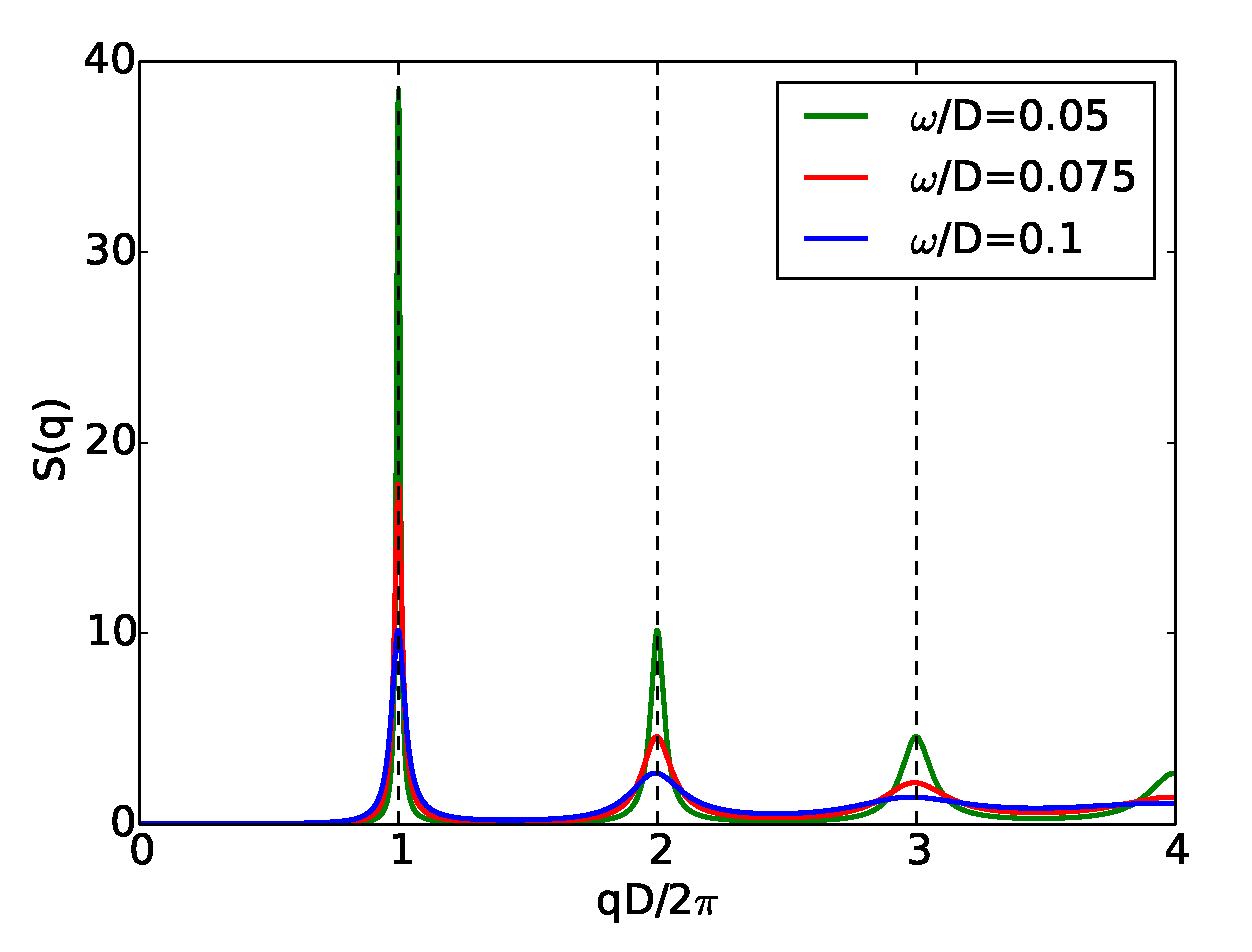
\includegraphics[width=0.6\textwidth]{fig/funcplot/S_q_1Dparacrystal.eps}
\end{center}
\caption{Interference function of a 1D Gaussian paracrystal plotted for different values of $\omega /D$. The peaks broaden with a decreasing amplitude as $\omega/D$ increases. This shows the transition between an ordered and a disordered states. }
\label{fig:1dparas_q}
\end{figure}

In two dimensions, the paracrystal is constructed on a pseudo-regular lattice with base vectors $\v{a}$ and $\v{b}$ using the following conditions for the densities of probabilities:\\
$\int p_{\v{a}}(\r)\d^2r=\int p_{\v{b}}(\r)\d^2r=1$,
$\int \r p_{\v{a}}(\r)\d^2r=\v{a}$,
$\int \r p_{\v{b}}(\r)\d^2r=\v{b}$.

In the ideal case the deformations along the two axes are decoupled
and each unit cell should retain a parallelogram shape.
The interference function is given by
$S(q_{\plll})=\prod_{k=a,b}\Re\left(\dfrac{1+P_k(q_{\plll})}{1-P_k(q_{\plll})} \right)$
with $P_k$ the Fourier transform of $p_k$, $k=a, b$.

\paragraph{Probability distributions} \mbox{}\\
The scattering by an ordered lattice gives rise to a series of Bragg peaks situated at the nodes of the reciprocal lattice. Any divergence from the ideal crystalline case modifies the output spectrum by, for example, widening or attenuating the Bragg peaks. The influence of these "defects" can be accounted for
 in direct space by using correlation functions or by truncating the lattice or, in reciprocal space with structure factors or interference functions by convoluting the scattered peaks with a function which could reproduce the experimental shapes.

%===============================================================================
\subsection{Size-Spacing Correlation Approximation}
%===============================================================================
\index{Size-spacing correlation approximation}

TO MERGE IN:
introduces correlations between polydisperse particles, more precisely between the size of the particles and their mutual spacing. A classical example would consist in particles whose closest-neighbor spacing depends linearly on the sum of their respective sizes \cite{LaLR07}, as illustrated in \cref{fig:ssca}.

%For a sample where only the statistical properties of particle positions and size are known, the scattered intensity per scattering particle is expressed as the average over an ensemble of the Fourier transform of the Patterson function, which is the autocorrelation of the SLD $\curlp (\r ) \equiv \sum_{ij} S_i(-\r )\otimes S_j(\r )\otimes \delta (\r + \r_i - \r_j )$:
%\begin{equation*}
%  I(\q ) = \frac{1}{N}\ensavg{}{\curlf (\curlp (\r ))},
%\end{equation*}
%where $\curlf$ denotes the Fourier transform and $\curlp$ the Patterson function

\begin{figure}[tb]
\begin{center}
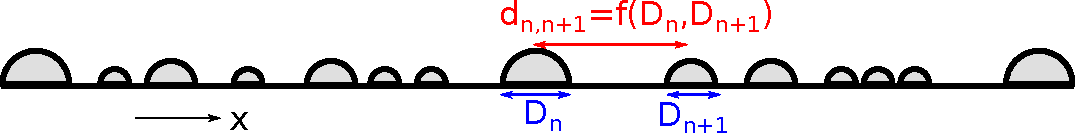
\includegraphics[width=0.9\textwidth]{fig/drawing/drawingSSCA.pdf}
\end{center}
\caption{Sketch of a 1D distributed collection of particles, whose scattering could be described by the size-spacing correlation approximation: the distance between two particles depends on their sizes.}
\label{fig:ssca}
\end{figure}


In the Size-Spacing Correlation Approximation, a correlation is assumed between the shape/size of the particles and their mutual spacing. A classical example would consist of particles whose closest-neighbor spacing depends linearly on the sum of their respective sizes. The following discussion of this type of correlation is inspired by \cite{LaLR07}

The scattered intensity can also be calculated as the Fourier transform of the Patterson function, which is the autocorrelation of the SLD:
\begin{equation*}
  \curlp (\r ) \equiv \sum_{ij} S_i(-\r )\otimes S_j(\r )\otimes \delta (\r + \r_i - \r_j ).
\end{equation*}
For a sample where only the statistical properties of particle positions and shape/size are known, the scattered intensity per scattering particle becomes average over an ensemble of the Fourier transform of the Patterson function:
\begin{equation*}
  I(\q ) = \frac{1}{N}\bra\curlf (\curlp (\r ))\ket,
\end{equation*}
where $\curlf$ denotes the Fourier transform.

The ensemble averaged Patterson function will be denoted as:
\begin{equation*}
  Z(r) \equiv \frac{1}{N}\bra\curlp (\r )\ket.
\end{equation*}
In the case of systems where the particles are aligned in one dimension, this autocorrelation function can be further split into nearest neighbor probabilities. First, it is split into terms for negative, zero or positive distance:
\begin{equation*}
  Z(\r ) \equiv z_0(\r ) + z_+(\r ) + z_-(\r ).
\end{equation*}
Taking $x$ as the coordinate in the direction in which the particles are arranged and $s$ as an orthogonal coordinate ($\r \equiv (x,s)$), one obtains:
\begin{align*}
  z_0(\r ) &= \sum_{\alpha_0} p(\alpha_0) S_{\alpha_0}(-x,-s) \otimes S_{\alpha_0}(x,s)  \\
  z_+(\r ) &= \sum_{\alpha_0\alpha_1} p(\alpha_0,\alpha_1) S_{\alpha_0}(-x,-s) \otimes S_{\alpha_1}(x,s) \otimes P_1(x|\alpha_0\alpha_1)  \\
               &+ \sum_{\alpha_0\alpha_1\alpha_2} p(\alpha_0,\alpha_1,\alpha_2) S_{\alpha_0}(-x,-s) \otimes S_{\alpha_2}(x,s) \otimes P_1(x|\alpha_0\alpha_1) \otimes P_2(x|\alpha_0\alpha_1\alpha_2)  \\
               &+ \dotsb \\
  z_-(\r ) &= z_+(-\r ),
\end{align*}
where $p(\alpha_0,\dotsc ,\alpha_n)$ denotes the probability of having a sequence of particles of the indicated sizes/shapes and $P_n(x|\alpha_0\dotsc\alpha_n)$ is the probability density of having a particle of type $\alpha_n$ at a (positive) distance $x$ of its nearest neighbor of type $\alpha_{n-1}$ in a sequence of the given order.

In the Size-Spacing Correlation Approximation, one assumes that the particle sequence probabilities are just a product of their individual fractions:
\begin{equation*}
  p(\alpha_0,\dotsc ,\alpha_n) = \prod_i p(\alpha_i),
\end{equation*}
and the nearest neighbor distance distribution is dependent only on the two particles involved:
\begin{equation*}
  P_n(x|\alpha_0\dotsc\alpha_n) = P_1(x|\alpha_{n-1}\alpha_n).
\end{equation*}
Furthermore, the distance distribution $P_1(x|\alpha_0\alpha_1)$ depends on the particle sizes/shapes only through its mean value $D$:
\begin{equation*}
  P_1(x|\alpha_0\alpha_1) = P_0(x - D(\alpha_0,\alpha_1) ),
\end{equation*}
where $D(\alpha_0,\alpha_1) = D_0 + \kappa \left[ \Delta R(\alpha_0) + \Delta R(\alpha_1) \right]$, with $\Delta R(\alpha_i)$ the deviation of a size parameter of particle $i$ with respect to the mean over all particles sizes/shapes and $\kappa$ the coupling parameter.

In momentum space, the sum of convolutions can be written as a geometric series, which can be exactly calculated to be:
\begin{equation}
\label{Esscainf}
I(\q ) = {\bra\left| F_\alpha(\q ) \right| ^2\ket}_{\alpha}
+ 2 \Re \left\lbrace \widetilde{\curlf_\kappa}(\q )
 \widetilde{\curlf_\kappa^*}(\q ) \cdot
 \frac{\Omega_\kappa(\q )}{\tilde{p}_{2\kappa}(\q )\left
   [ 1 - \Omega_\kappa(\q )\right] } \right\rbrace,
\end{equation}
with
\begin{align*}
  \tilde{p}_\kappa(\q ) &= \int \d\alpha\; p(\alpha) \e^{i\kappa q_x \Delta R(\alpha)}  \\
  \Omega_\kappa(\q ) &= \tilde{p}_{2\kappa}(\q ) \phi(\q) \e^{i q_x D_0}  \\
  \widetilde{\curlf_\kappa}(\q ) &=
       \int \d\alpha\; p(\alpha)F_\alpha (\q ) \e^{i\kappa q_x \Delta R(\alpha)},
\end{align*}
and the Fourier transform of $P_1(x|\alpha_0\alpha_1)$ is
\begin{equation*}
  \curlp (\q ) = \phi (\q )\e^{i q_x D_0}
                    \e^{i \kappa q_x \left[ \Delta R(\alpha_0) + \Delta R(\alpha_1) \right] }.
\end{equation*}

Using the result from the one-dimensional analysis, one can apply this formula ad hoc for distributions of particles in a plane, where the coordinate $x$ will now be replaced with $(x,y)$, while the $s$ coordinate encodes a position in the remaining orthogonal direction. One must be aware however that this constitutes a further approximation, since this type of correlation does not have a general solution in more than one dimension.

The intensity in \cref{Esscainf} will contain a Dirac delta function contribution, caused by taking an infinite sum of terms that are perfectly correlated at $\q = 0$. One can leverage this behaviour by multiplying the nearest neighbor distribution by a constant factor $\e^{-D/\Lambda}$, which removes the division by zero in \cref{Esscainf}.
Another way of dealing with this infinity at $\q =0$ consists of taking only a finite number of terms, in which case the geometric series still has an analytic solution, but becomes a bit more cumbersome:
\begin{equation*}
\begin{split}
  I(\q ) &= {\bra\left| F_\alpha(\q ) \right| ^2\ket}_\alpha
   + 2 \Re \Biggl\lbrace \frac{1}{\tilde{p}_{2\kappa}(\q )}\widetilde{\curlf_\kappa}(\q )\widetilde{\curlf_\kappa^*}(\q ) \\
  & \times \left[ \left( 1 - \frac{1}{N}\right) \frac{\Omega_\kappa(\q )}{1 - \Omega_\kappa(\q ) } - \frac{1}{N}\frac{\Omega_\kappa^2(\q )\left( 1- \Omega_\kappa^{N-1}(\q )\right) }{\left( 1 - \Omega_\kappa(\q ) \right) ^2 } \right] \Biggr\rbrace.
\end{split}
\end{equation*}
This expression has a well-defined limit for $\Omega_\kappa(\q ) \rightarrow 1$ (when $\q \rightarrow 0$), namely:
\begin{equation*}
  \lim_{\q \rightarrow 0} I(\q ) = {\bra\left| F_\alpha(0 ) \right| ^2\ket}_{\alpha} + \left( N-1 \right) \left| {\bra F_\alpha(0 )\ket}_{\alpha} \right|^2.
\end{equation*}


%%%%%%%%%%%%%%%%%%%%%%%%%%%%%%%%%%%%%%%%%%%%%%%%%%%%%%%%%%%%%%%%%%%%%%%%%%%%%%%%
\section{Vertical location of particles}
%%%%%%%%%%%%%%%%%%%%%%%%%%%%%%%%%%%%%%%%%%%%%%%%%%%%%%%%%%%%%%%%%%%%%%%%%%%%%%%%

 \Note{The particles cannot sit in between layers. At most they can be sitting on any inner interfaces.}

%===============================================================================
\subsection{Particles deposited on a substrate}
%===============================================================================
%Substrate modified Born approximation
In this configuration, the particles are sitting on top of a substrate layer in air or vacuum.
In the DWBA the expression of a form factor becomes
\begin{align}
F_{\rm{DWBA}}(q_{\plll}, k_{i,z}, k_{f,z}) &= F_{\rm{BA}}(q_{\plll}, k_{i,z}-k_{f,z})+ R_i F_{\rm{BA}}(q_{\plll}, -k_{i,z}-k_{f,z}) \nonumber \\
&+ R_f F_{\rm{BA}}(q_{\plll}, k_{i,z}+k_{f,z}) + R_i R_f F_{\rm{BA}}(q_{\plll},-k_{i,z}+k_{f,z}), \label{Edwbaair}
\end{align}
where $q_{\plll}$ is the component of the scattering beam in the plane of the interface ($\q=\k_i-\k_\sf$), $k_{i,z}$ and $k_{f,z}$ are the z-component of the incident and scattered beam, respectively. $R_i$, $R_f$ are the reflection coefficients in incidence and reflection. They are defined as\\ $R=\dfrac{k_z+\sqrt{n_s^2k_0^2-|k_{\plll}|^2}}{k_z-\sqrt{n_s^2 k_0^2-|k_{\plll}|^2}}$, where $n_s=1-\delta_s +i \beta_s$ is the refractive index of the substrate, $k_0$ is the wavelength in vacuum ($2\pi /\lambda$), $k_z$ and $k_{\plll}$ are the $z$-component and the in-plane component of $\k_\si$ or $\k_\sf$. \\

\Note{If the particles are sitting on a multilayered system, the expression of the form factor in the DWBA is obtained by replacing the Fresnel coefficient by the corresponding coefficients of the underlying layers \cite{Par54,BoWo99}.}

Script~\ref{lst:badwba} illustrates the difference between BA and DWBA in \BornAgain\ when generating the sample.  We consider the simple case of:
\begin{itemize}
\item one kind of particles' shape,
\item no interference between the particles,
\item in the DWBA, a sample made of a layer of substrate on which are deposited the particles,
\item in the BA, a sample composed of the particles in air.
\end{itemize}

\Cref{fig:spheroidbadwba} shows the intensity contour plot generated using this script with truncated spheroids as particles.

\newpage

\begin{lstlisting}[language=python, style=eclipseboxed,numbers=none,nolol,caption={\Code{Python} script to generate a sample using Born (BA) or distorted-wave Born approximation (DWBA). The difference between BA and DWBA in this simple case is the absence or presence of a substrate layer in the sample.},label={lst:badwba}]
def get_sample():
    """
    Build and return the sample to calculate form factor of
    truncated spheroid in Born or distorted-wave Born Approximation.
    """
    # defining materials
    m_ambience = HomogeneousMaterial("Air", 0.0, 0.0)
    m_substrate = HomogeneousMaterial("Substrate", 6e-6, 2e-8)
    m_particle = HomogeneousMaterial("Particle", 6e-4, 2e-8)

    # collection of particles
    ff= FormFactorTruncatedSpheroid(7.5*nanometer, 9.0*nanometer, 1.2)
    particleshape = Particle(m_particle, ff)
    particle_layout = ParticleLayout()
    particle_layout.addParticle(particleshape, 1.0)

    # interferences
    interference = InterferenceFunctionNone()
    particle_layout.addInterferenceFunction(interference)

    # assembling the sample
    air_layer = Layer(m_ambience)
    air_layer.addLayout(particle_layout)
    substrate_layer = Layer(m_substrate, 0)

    multi_layer = MultiLayer()
    multi_layer.addLayer(air_layer)
    # Comment the following line out for Born Approximation
    multi_layer.addLayer(substrate_layer)
    return multi_layer
\end{lstlisting}


\begin{figure}[tb]
\hfill
\subfigure[Born Approximation]{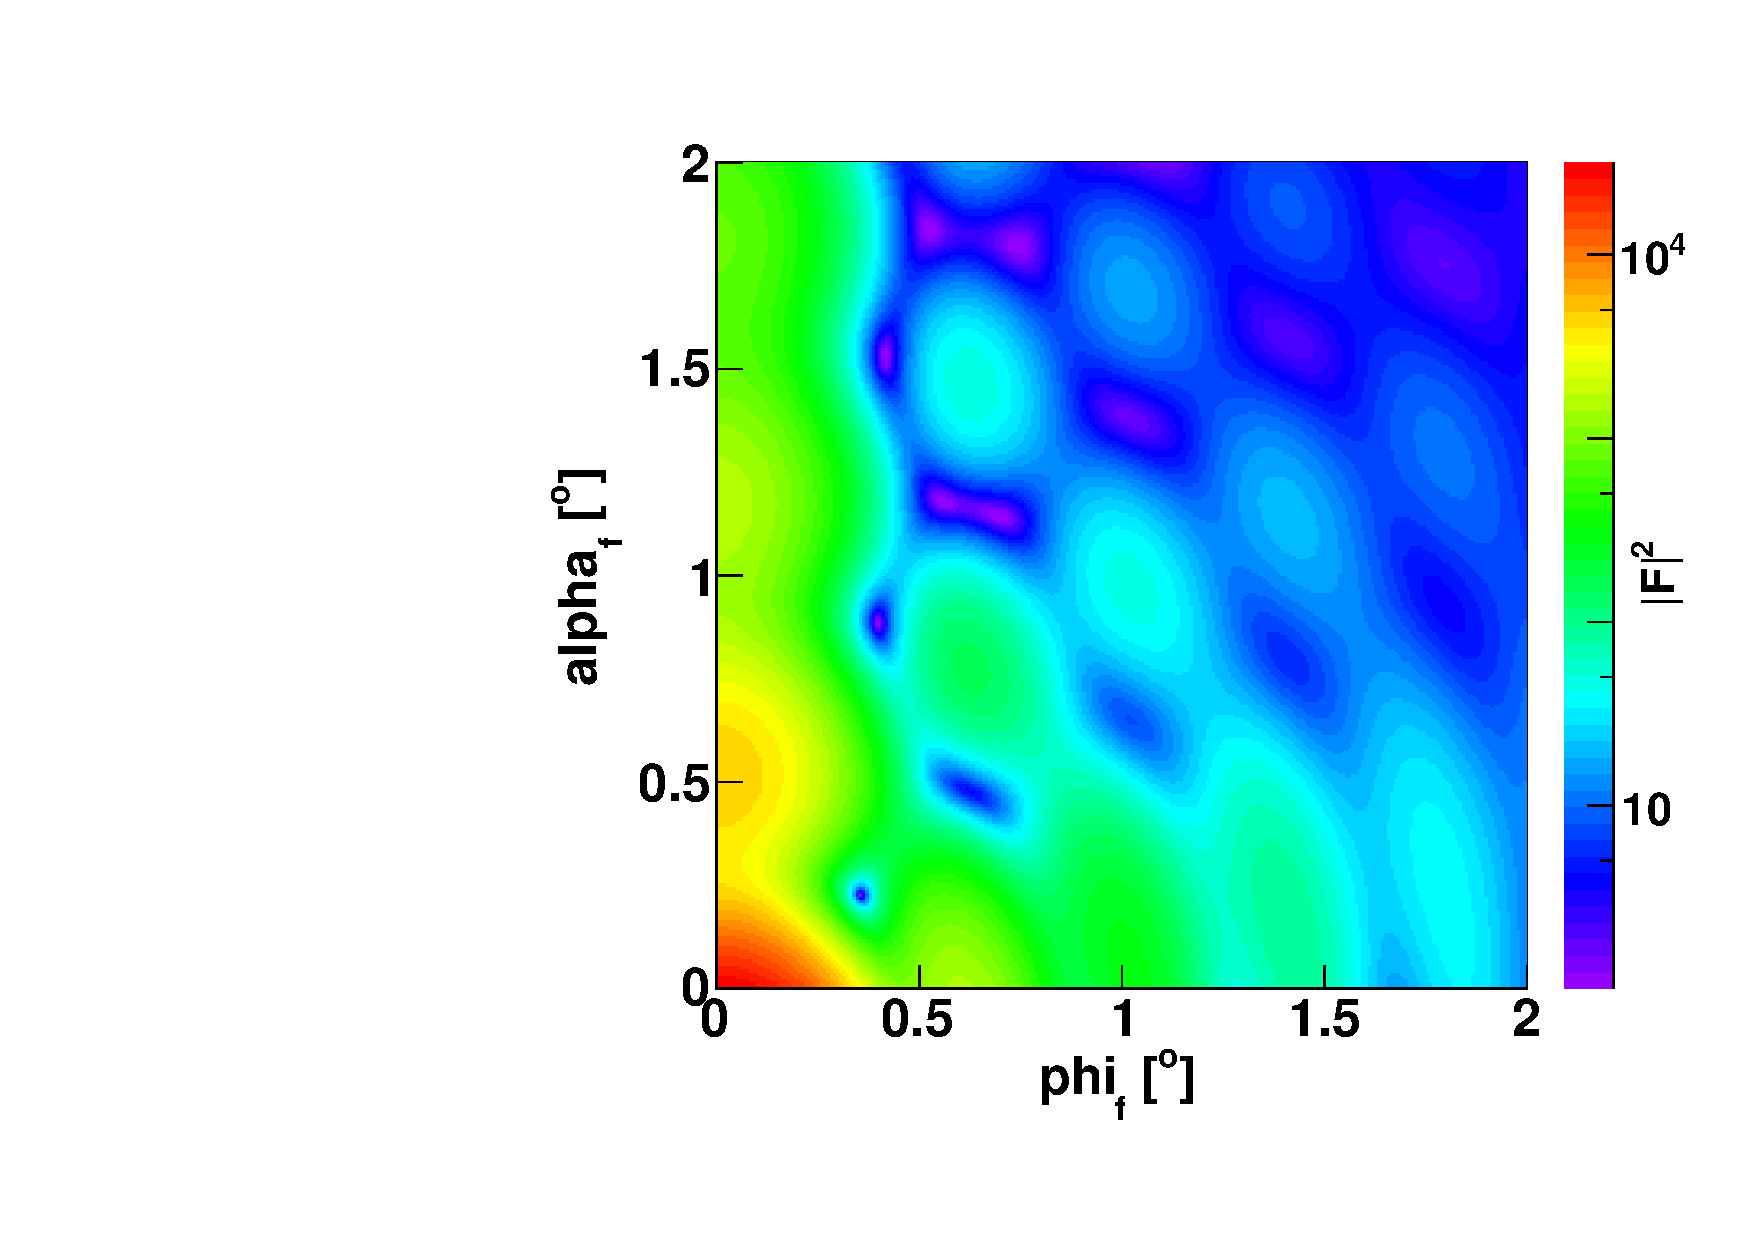
\includegraphics[angle=-90,width=6cm]{fig/gisasmap/ffspheroidBA.pdf}}
\hfill
\subfigure[DWB Approximation]{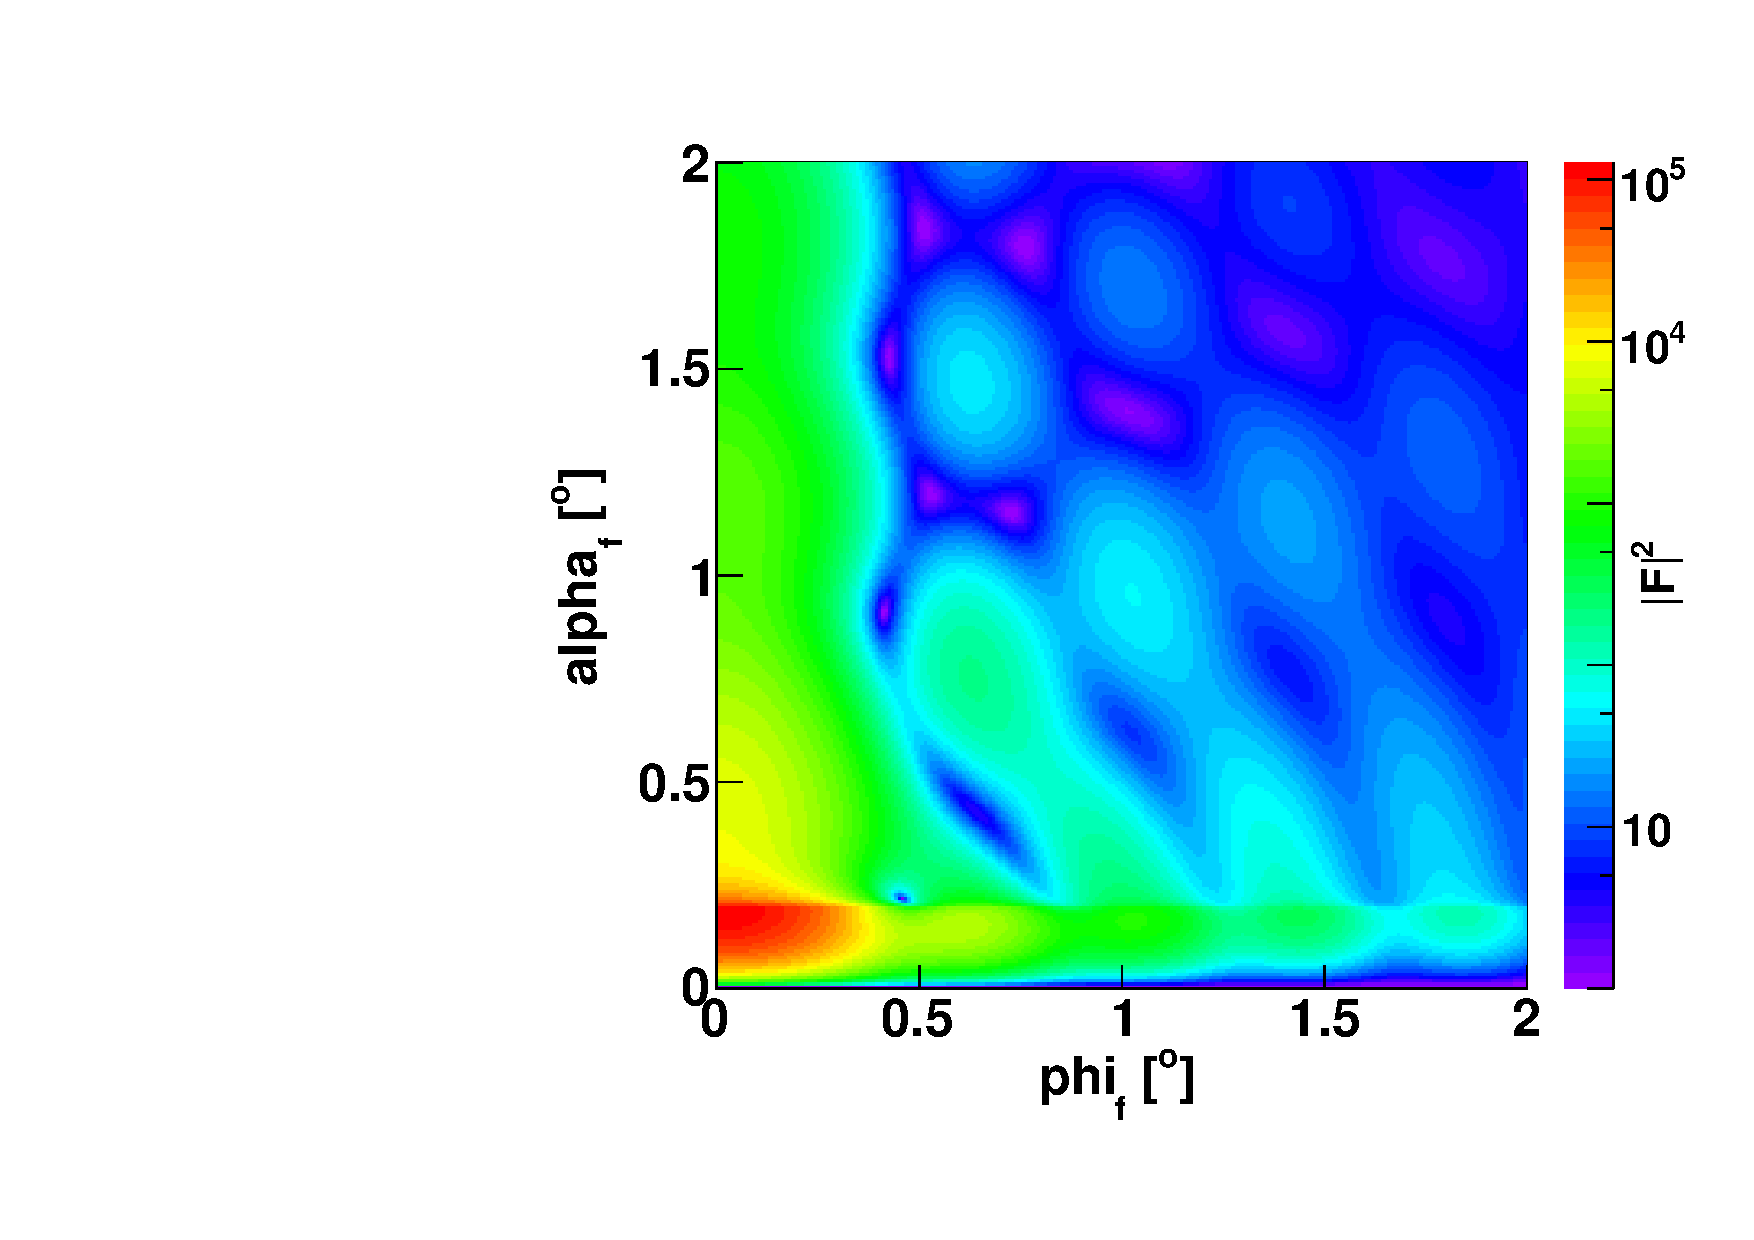
\includegraphics[angle=-90,width=6cm]{fig/gisasmap/ffspheroidDWBA.pdf}}
\hfill
\caption{Intensity map of TruncatedSpheroid form factor in BA and DWBA computing using script~\ref{lst:badwba} for the sample.}
\label{fig:spheroidbadwba}
\end{figure}

\FloatBarrier

\Note{In \BornAgain, the DWBA is implemented automatically when assembling the sample with more layers than only the air layer (for example, for particles are sitting on a substrate).}

%===============================================================================
\subsection{Buried particles}
%===============================================================================

The system considered in this section consists of particles encapsulated in a layer, which is sitting on a substrate. In this case the form factor in the DWBA is given by

\begin{align}
  F_{\rm{DWBA}}(q_{\plll}, k_{i,z}, k_{f,z})
  &= T_\si T_\sf F_{\rm{BA}}(q_{\plll}, k_{i,z}-k_{f,z})\e^{i(k_{i,z}-k_{f,z})d}\nonumber \\
  &+ R_\si T_\sf F_{\rm{BA}}(q_{\plll}, -k_{i,z}-k_{f,z})\e^{i(-k_{i,z}-k_{f,z})d} \nonumber \\
  &+ R_\sf T_\si F_{\rm{BA}}(q_{\plll}, k_{i,z}+k_{f,z}) \e^{i(k_{i,z}+k_{f,z})d}\nonumber \\
  &+ R_\sf R_\si F_{\rm{BA}}(q_{\plll},-k_{i,z}+k_{f,z})\e^{i(-k_{i,z}+k_{f,z})d}, \label{Edwbaburied}
\end{align}

\begin{equation*}
R_j =\frac{t^{j}_{0,1}r^{j}_{1,2}\exp(2ik_{j,z}t)}{1+r^{j}_{0,1}r^{j}_{1,2}\exp(2ik_{j,z}t)}, \quad T_j=\frac{t^{j}_{0,1}}{1+r^{j}_{0,1}r^{j}_{1,2}\exp(2ik_{j,z}t)}, j=i,f
\end{equation*}
where $q_{\plll}$ is the component of the scattering beam in the plane of the interface, $k_{i,z}$ and $k_{f,z}$ are the z-component of the incident and scattered beams, respectively.  $d$ is the depth at which the particles are sitting in the layer. Note that this value is given relative to the top of this layer and it is not the coordinate in the absolute referential (linked with the full sample) and it is measured up to the bottom of the particle. $t$ is the thickness of the intermediate layer containing the particles. $R_{i,f}$ and $T_{i,f}$  are the reflection  and transmission coefficients in incidence and reflection (they can be calculated using Parratt or matrix formalism). $r^j_{0,1}$, $r^j_{1,2}$ $t^j_{0,1}$ are the reflection and transmission coefficients between layers; the indices are related to different boundaries with 0: air, 1: intermediate layer and 2: substrate layer and the superscript $j$ is associated with the incident or scattered beams:
\begin{equation*}
r^j_{n,n+1}=\frac{k_{j,z,n}-k_{j,z,n+1}}{k_{j,z,n}-k_{j,z,n+1}}, \qquad t^j_{n,n+1}= \frac{2k_{j,z,n}}{k_{j,z,n}-k_{j,z,n+1}}, \quad n=0,1, \quad j=i,f,
\end{equation*}
where index $n$ is related to the layers, $z$ to the vertical component, and $j$ to the beams (incident and outgoing).

\Cref{fig:dwbaburied} shows a typical example of the output intensity scattered from a sample made of 3 layers: air, substrate, and in between, spherical particles embedded in the middle of a 30~nm-thick layer. This figure had been generated using listing~\ref{lst:dwbaburied}.

\begin{lstlisting}[language=python, style=eclipseboxed,numbers=none,nolol,caption={\Code{Python} script to generate a sample where spherical particles are embedded in the middle of a layer on a substrate.},label={lst:dwbaburied}]
def get_sample():
    """
    Build and return the sample with buried spheres in DWBA.
    """
    # defining materials
    m_ambience = HomogeneousMaterial("Air", 0.0, 0.0)
    m_interm_layer = HomogeneousMaterial("IntermLayer",3.45e-6, 5.24e-9)
    m_substrate = HomogeneousMaterial("Substrate", 7.43e-6, 1.72e-7)
    m_particle = HomogeneousMaterial("Particle", 0.0, 0.0)

    # collection of particles
    ff = FormFactorFullSphere(10.2*nanometer)
    particleshape = Particle(m_particle, ff)
    particleshape.setPosition(0.0, 0.0, -25.2)
    particle_layout = ParticleLayout()
    particle_layout.addParticle(particleshape, 1.0)

    # interferences
    interference = InterferenceFunctionNone()
    particle_layout.addInterferenceFunction(interference)

    # assembling the sample
    air_layer = Layer(m_ambience)
    intermediate_layer = Layer(m_interm_layer, 30.*nanometer)
    intermediate_layer.addLayout(particle_layout)
    substrate_layer = Layer(m_substrate, 0)

    multi_layer = MultiLayer()
    multi_layer.addLayer(air_layer)
    multi_layer.addLayer(intermediate_layer)
    multi_layer.addLayer(substrate_layer)
    return multi_layer
\end{lstlisting}


\begin{figure}[tb]
\centering
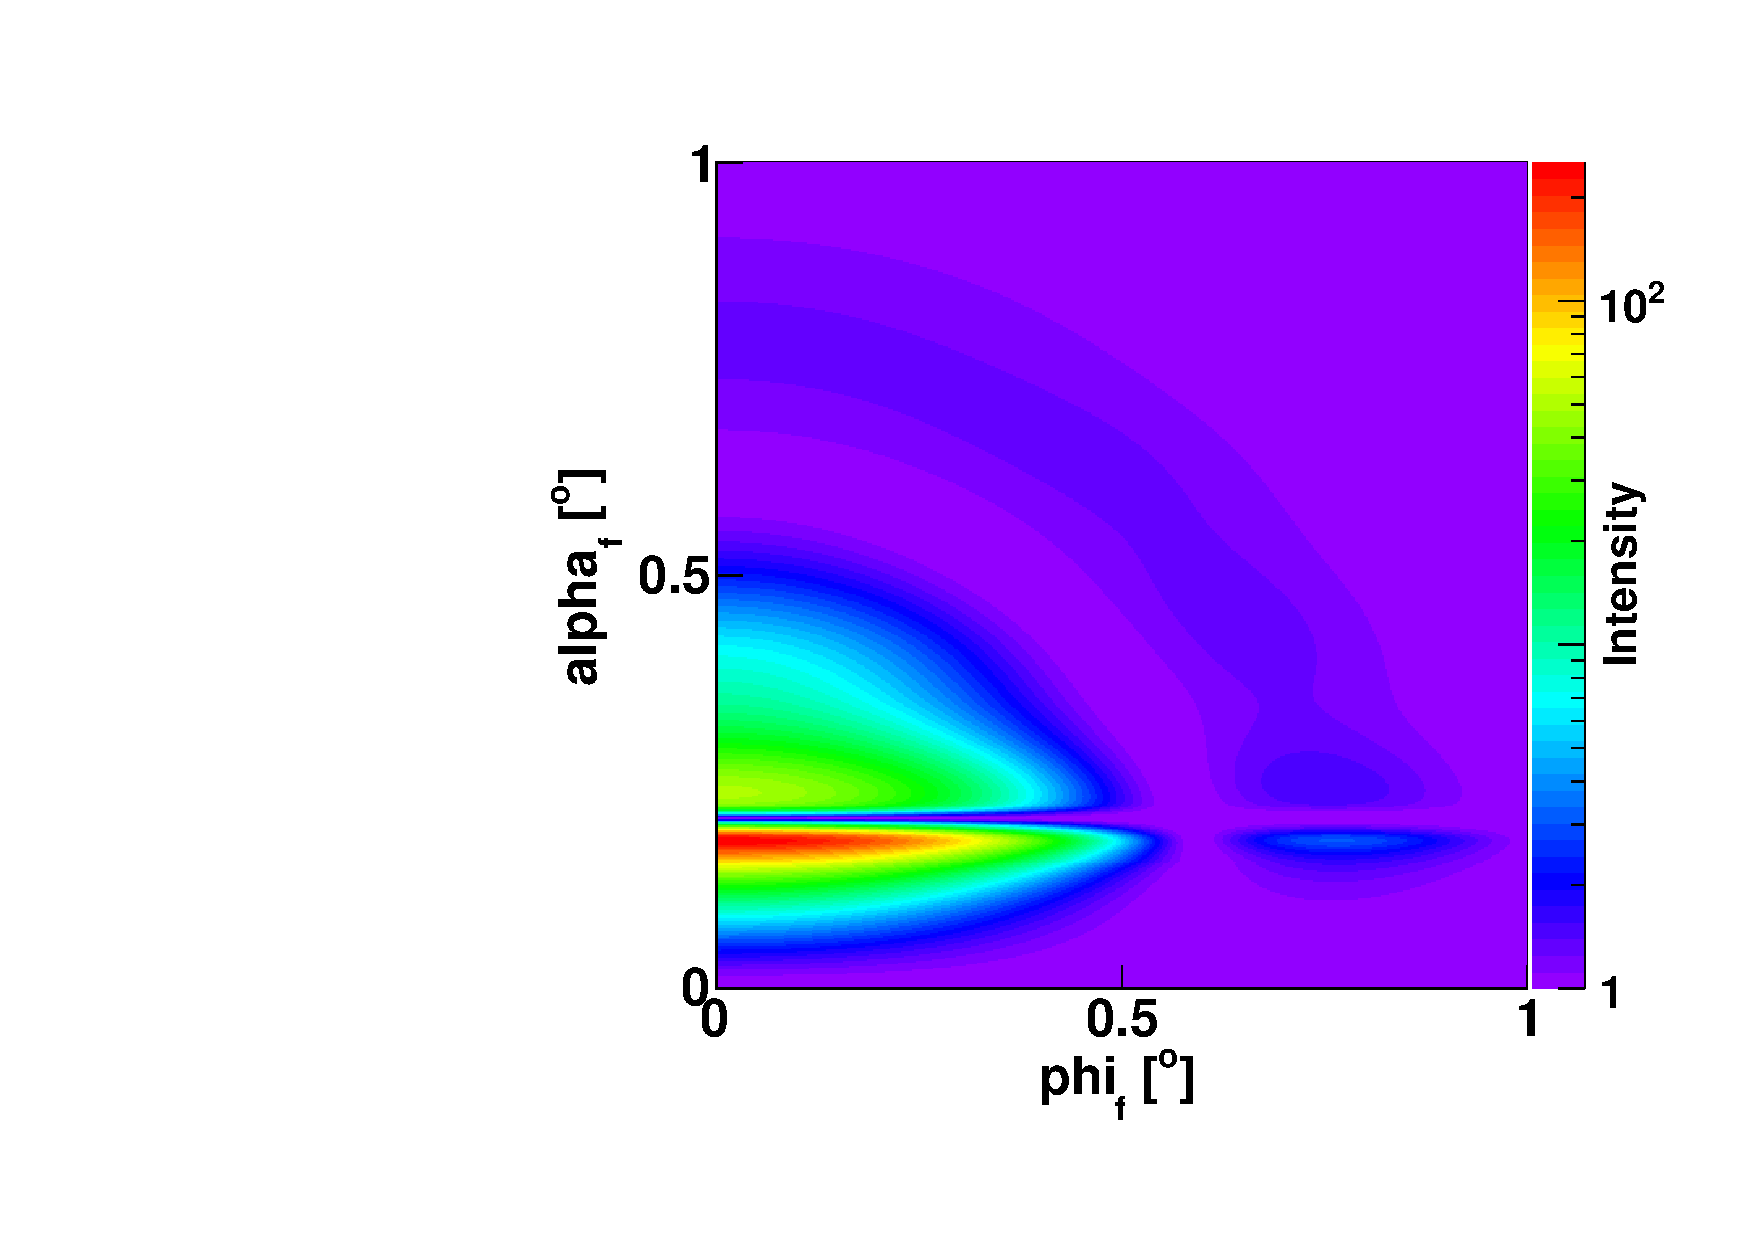
\includegraphics[angle=-90,width=0.6\textwidth]{fig/gisasmap/figIntBuriedPart.pdf}
\caption{Map of intensity scattered from a sample made of spherical particles embedded in the middle of a 30~nm-thick layer on a substrate (see Script~\ref{lst:dwbaburied} for details about the sample).}
\label{fig:dwbaburied}
\end{figure}

\newpage

\Note{For layers different from the air layer, the top interface is considered as the reference level to position the encapsulated particles. For example, spheres positioned at depth $d$ (positive) are located at a distance $d$ from the top of the layer up to the bottom of these particles. This convention is different for the top air layer, where particles sitting at the interface with an underlying layer (\idest the bottom of the air layer) are located at depth 0 (see \cref{fig:depthpartBA}).}


\begin{figure}[tb]
\centering
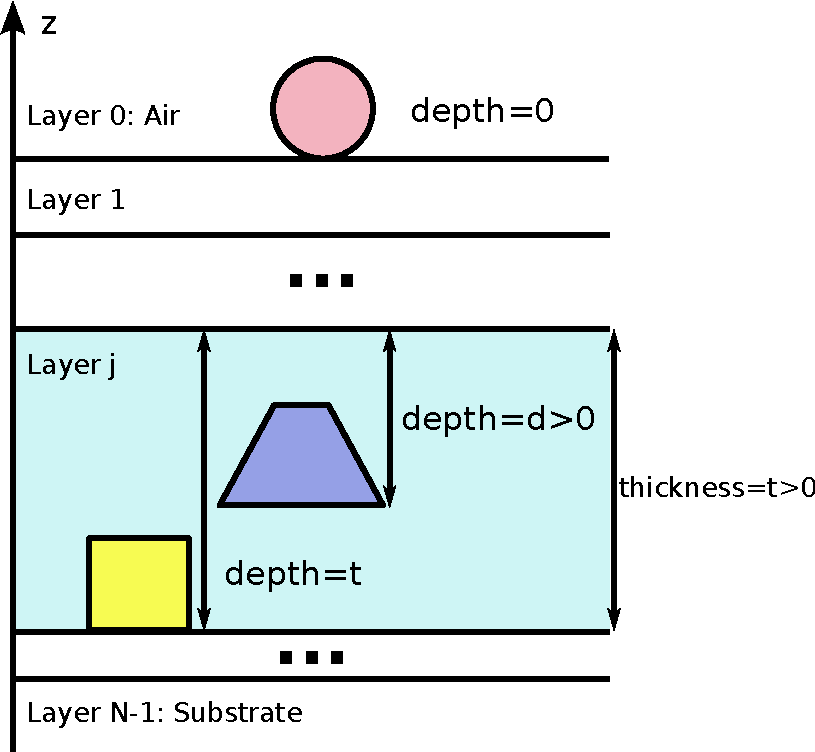
\includegraphics[width=0.5\textwidth]{fig/drawing/drawingDepthParticle.pdf}
\caption{Illustration of the convention about \Code{depth} used in \BornAgain\ to encapsulate particles in layers.}
\label{fig:depthpartBA}
\end{figure}


%%%%%%%%%%%%%%%%%%%%%%%%%%%%%%%%%%%%%%%%%%%%%%%%%%%%%%%%%%%%%%%%%%%%%%%%%%%%%%%%
\section{Implementation in \BornAgain}
%%%%%%%%%%%%%%%%%%%%%%%%%%%%%%%%%%%%%%%%%%%%%%%%%%%%%%%%%%%%%%%%%%%%%%%%%%%%%%%%

This section describes the implementation of the interference functions in \BornAgain.
For an implementation of all the components of a simulation,
the use is referred, for example, to \cref{sec:Example1Python}.\\


\Note{In \BornAgain\ the particles are positioned in the same vertical layer.}

\subsection{Size-distribution models}
\index{Size-distribution models}
The decoupling approximation (DA), local monodisperse approximation (LMA) and size spacing correlation approximation (SSCA) can be used in \BornAgain.
The selection between DA and SSCA is made using\\
\Code{ILayout.setApproximation(EInterferenceFunction approximation)} when defining the characteristics of the way particles and interference functions are embedded in a layer.  For example,
\begin{lstlisting}[language=python, style=eclipseboxed,numbers=none,nolol]
    particle_layout = ParticleLayout()
   ....
# interference approx chosen between: DA (default) and SSCA
    particle_layout.setApproximation(ILayout.DA)
\end{lstlisting}

Note that with the SSCA, the users have to specify the coupling parameter $\kappa$ (with the function \Code{setKappa}), which should be a positive dimensionless value. $\kappa$ characterizes the influence of the neighboring particles' sizes on their distance. If $\kappa=0$, the SSCA reduces to the DA with a radial paracrystal for the interference function.\\

For the LMA, its implementation is automatically done when using more than one layout of particles:
\begin{lstlisting}[language=python, style=eclipseboxed,numbers=none,nolol]
    particle_layout0 = ParticleLayout()
    particle_layout1 = ParticleLayout()
   ....
# association of each particles' layout with materials, form factors
#... and with a material layer
    layer_a = Layer(m_material_a)
    layer_a.addLayout(particle_layout0)
    layer_a.addLayout(particle_layout1)
\end{lstlisting}

%%ADD EXPLANATION ABOUT LMA

%-------------------------------------------------------------------------------
\subsection{Probability distribution functions}\label{baftd}
%-------------------------------------------------------------------------------

The probability distribution functions have been implemented in the reciprocal space in \BornAgain. Their expressions are given in Table~\ref{table:pdf}.

\begin{table}[H]
\centering
\begin{tabular}{ccc}
\hline
Function & One dimension & Two dimensions\\
\hline
Cauchy & $(1+q^2\omega^2)^{-3/2}$ & $(1 + q_x^2 cl_x^2 + q_y^2 cl_y^2)^{-3/2}$ \\
Gauss & $\dfrac{1}{2}\exp(-\dfrac{q^2\omega^2}{4})$ & $\frac{1}{2}\exp\left(-\dfrac{q_x^2 cl_x^2+ q_y^2cl_y^2}{4}\right)$ \\
Voigt & $\dfrac{\eta}{2} \exp\left(-\dfrac{q^2\omega^2}{4}\right) + \dfrac{1 - \eta}{(1 + q^2\omega^2)^{3/2}}$ & $\dfrac{\eta}{2} \exp\left(-\dfrac{q_x^2 cl_x^2+ q_y^2cl_y^2}{4}\right)+ \dfrac{1 - \eta}{(1 + q_x^2 cl_x^2+ q_y^2cl_y^2)^{3/2}}$ \\
\hline
\end{tabular}
\caption{List of probability distribution functions in reciprocal space. $\omega$, $cl$ stand for coherence lengths (the index refers to the axis) and  $\eta$ is a weighting coefficient.}
\label{table:pdf}
\end{table}

The Cauchy distribution corresponds to $\exp(-r)$ in real space and the Voigt one  is a linear combination of the Gaussian and Cauchy probability distribution functions.\\

\noindent \underline{One dimension}
\begin{itemize}
\item \Code{FTDistribution1DCauchy($\omega$)},
\item \Code{FTDistribution1DGauss($\omega$)},
\item \Code{FTDistribution1DVoigt($\omega, \eta$)}.
\end{itemize}
where $\omega$ is the coherence length and $\eta$ is a weighting factor.\\

\noindent \underline{Two dimensions}
\begin{itemize}
\item \Code{FTDistribution2DCauchy($cl_x$, $cl_y$)},
\item \Code{FTDistribution2DGauss($cl_x$, $cl_y$)},
\item \Code{FTDistribution2DVoigt($cl_x$, $cl_y$)}
\end{itemize}
where $cl_{x,y}$ are the coherence lengths in the $x$ or $y$ direction, respectively.

These functions can be used with all interference functions, except the case without any interference.

%-------------------------------------------------------------------------------
\subsection{Interferences}
%-------------------------------------------------------------------------------
\index{Interference function}

The interference function is specified when building the sample. It is linked with the particles (shape, material). Examples of implementation are given at the end of each description.

\paragraph{Syntax:}
 \Code{particle\_layout.addInterferenceFunction(interference\_function)},\\ where \Code{particle\_layout} holds the information about the different shapes and their proportions for a given layer of particles, and \Code{interference\_function}  is one of the following expressions:
\begin{itemize}
\item \Code{InterferenceFunctionNone()}
\item \Code{InterferenceFunction1DLattice(lattice\_parameters)}
\item \Code{InterferenceFunctionRadialParaCrystal(peak\_distance, damping\_length)}
\item \Code{InterferenceFunction2DLattice(lattice\_parameters)}
\item \Code{InterferenceFunction2DParaCrystal(length\_1, length\_2, $\alpha$\_lattice, $\xi$, \\ damping\_length)}
\end{itemize}

\Note{\Code{InterferenceFunction1DLattice} can only be used for particles which are infinitely long in one direction of the sample's surface like for example a rectangular grating.}

\newpage
%-------------------------------------------------------------------------------
\subsection{InterferenceFunctionNone}
%-------------------------------------------------------------------------------

The particles are placed randomly in the dilute limit and are considered as individual, non-interacting scatterers. The scattered intensity is function of the form factors only.

\paragraph{Example} The sample is made of a substrate on which are deposited half-spheres. Script~\ref{lst:nointerf} details the commands necessary to generate such a sample. \Cref{fig:nointerf} shows an example of output intensity: Script~\ref{lst:nointerf}  + detector's + input beam's characterizations.


\begin{figure}[tb]
\begin{center}
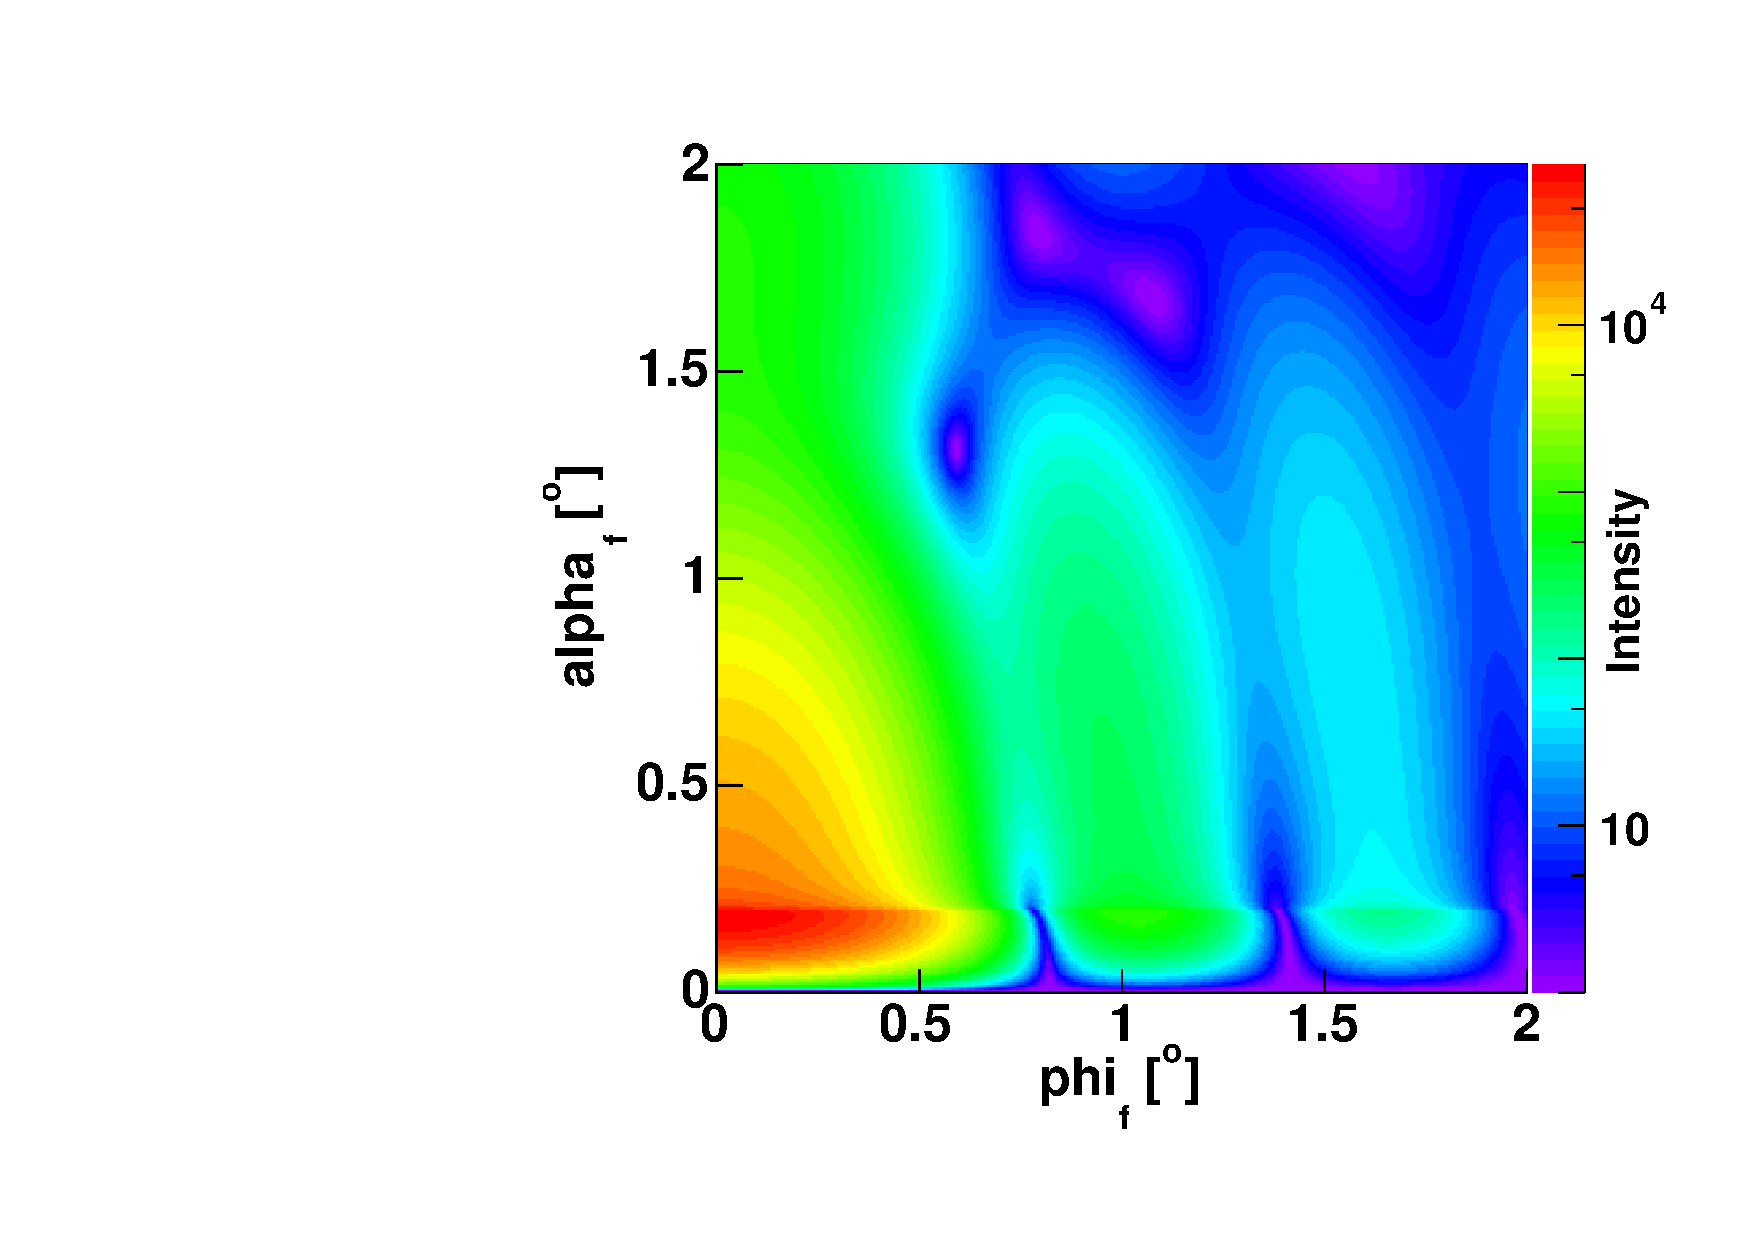
\includegraphics[angle=-90,width=0.5\textwidth]{fig/gisasmap/HSphere_NoInterf.pdf}
\end{center}
\caption{Output intensity scattered from a sample made of half-spheres with no interference between them.}
\label{fig:nointerf}
\end{figure}

\FloatBarrier
\newpage

\begin{lstlisting}[language=python, style=eclipseboxed,numbers=none,nolol,caption={\Code{Python} script to simulate a sample made of half-spheres deposited on a substrate layer without any interference. The part specific to the interferences is marked in a red italic font.},label={lst:nointerf}]
def get_sample():
    """
    Build and return the sample representing particles with no interference
    """
    # defining materials
    m_ambience = HomogeneousMaterial("Air", 0.0, 0.0)
    m_substrate = HomogeneousMaterial("Substrate", 6e-6, 2e-8)
    m_particle = HomogeneousMaterial("Particle", 6e-4, 2e-8)
    # collection of particles
    sphere_ff = FormFactorTruncatedSphere(5*nanometer, 5*nanometer)
    sphere = Particle(m_particle, sphere_ff)
    particle_layout = ParticleLayout()
    particle_layout.addParticle(sphere, 1.0)
    |interference = InterferenceFunctionNone()|
    |particle_layout.addInterferenceFunction(interference)|
    # assembling the sample
    air_layer = Layer(m_ambience)
    air_layer.addLayout(particle_layout)
    substrate_layer = Layer(m_substrate, 0)

    multi_layer = MultiLayer()
    multi_layer.addLayer(air_layer)
    multi_layer.addLayer(substrate_layer)
    return multi_layer
\end{lstlisting}

\newpage
%-------------------------------------------------------------------------------
\subsection{\Code{InterferenceFunction1DLattice(lattice\_length, xi)}}
%-------------------------------------------------------------------------------
where lattice\_length is the lattice constant and $\xi$ the angle in radian between the lattice unit vector and the $\v{x}$-axis of the reference Cartesian frame as shown in \cref{fig:1dgrating}.

\begin{figure}[tb]
\begin{center}
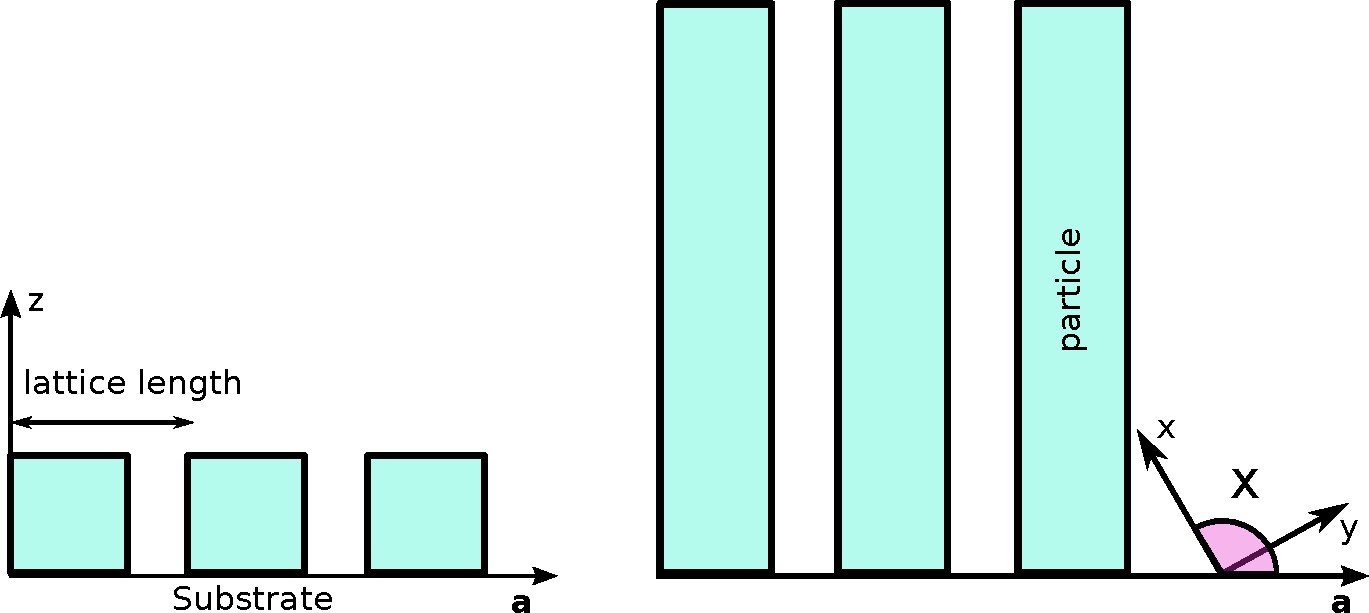
\includegraphics[width=0.75\textwidth]{fig/drawing/1DGrating.pdf}
\end{center}
\caption{Schematic representation of a 1D lattice (side and top views). Such a lattice is characterized by a lattice length and the angle $\xi$.}
\label{fig:1dgrating}
\end{figure}

\Note{By default the long axis of the particles in this 1D lattice is along the beam axis. That is the reason why in the example below the particles are rotated by  $90^{\circ}$ in the $(x,y)$ plane: the main axis of the lattice is therefore parallel to the y-axis, perpendicular to the long axis of the particles.}

\vspace{12pt}
A probability distribution function \Code{pdf} has to be chosen from the list in \cref{baftd} in order to apply some modifications to the scattering peaks. This function is implemented using \Code{setProbabilityDistribution(pdf)}.

\paragraph{Example:} Script~\ref{lst:1dlattinterf} details how to build in  \BornAgain\ a sample using\\ \Code{InterferenceFunction1DLattice} as the interference function. As mentioned previously, this interference function can only be used with infinitely wide or long particles.\\ Here the sample is made of infinitely long boxes deposited on a substrate (these particles are characterized by their widths and heights). They are also rotated by $90^{\circ}$  in the sample surface in order to have their long axis perpendicular to the input beam, which is along the $x$-axis.\\
 The lattice parameters (the lattice length and angle between the lattice main axis and the $x$-axis) are passed into the constructor of the interference function.

\newpage
\begin{lstlisting}[language=python, style=eclipseboxed,numbers=none,nolol,caption={\Code{Python} script to generate a sample made of infinitely long boxes deposited on a substrate layer with the 1DLatticeInterference function. The part specific to the interferences is marked in a red italic font.},label={lst:1dlattinterf}]
def get_sample():
    """
    Build and return the sample with 1DLatticeInterference function
    """
    # defining materials
    m_air = HomogeneousMaterial("Air", 0.0, 0.0)
    m_substrate = HomogeneousMaterial("Substrate", 6e-6, 2e-8)
    m_particle = HomogeneousMaterial("Particle", 6e-4, 2e-8)

    # collection of particles
    ff = FormFactorInfLongBox(10.*nanometer, 15.0*nanometer)
    box = Particle(m_particle, ff)
    particle_layout = ParticleLayout()
    transform = Transform3D.createRotateZ(90.0*degree)
    particle_layout.addParticle(box, transform)

    # interference function
    |interference = InterferenceFunction1DLattice(30.0*nanometer, 0.0*degree)|
    |pdf = FTDistribution1DCauchy(200./2./M_PI*nanometer)|
    |interference.setProbabilityDistribution(pdf)|
    |particle_layout.addInterferenceFunction(interference)|

    # air layer with particles and substrate form multi layer
    air_layer = Layer(m_air)
    air_layer.addLayout(particle_layout)
    substrate_layer = Layer(m_substrate, 0)

    multi_layer = MultiLayer()
    multi_layer.addLayer(air_layer)
    multi_layer.addLayer(substrate_layer)
    return multi_layer
\end{lstlisting}

\newpage
%-------------------------------------------------------------------------------
\subsection{\Code{InterferenceFunctionRadialParaCrystal(peak\_distance, damping\_length)}}
%-------------------------------------------------------------------------------
\begin{itemize}
\item[where] \Code{peak\_distance} is the average distance to the first neighbor peak,
\item[]\Code{width} is the width parameter of the probability distribution,
\item[] \Code{damping\_length} is used to introduce finite size effects by applying a multiplicative coefficient equal to  $\exp$(-\Code{peak\_distance/damping\_length}) to the Fourier transform of the probability densities. \Code{damping\_length} is equal to 0 by default and, in this case, no correction is applied.
\end{itemize}

A probability distribution function \Code{pdf} has to be chosen from the list in \cref{baftd} in order to apply some modifications to the scattering peaks. This function is implemented using \Code{setProbabilityDistribution(pdf)}.


\Note{
This interference function is not one-dimensional.  It takes into account the radial component of the scattering vector.
}

\paragraph{Example}
To illustrate the radial paracrystal interference function, we use the same sample as in the case without interference: half-spheres deposited on a substrate.

\begin{lstlisting}[language=python, style=eclipseboxed,numbers=none,nolol,caption={\Code{Python} script to define the radial paracrystal interference function between half-spheres, where \Code{trsphere} is of type \Code{Particle}.},label={lst:1dpara}]
    particle_layout = ParticleLayout()
    particle_layout.addParticle(trsphere, 1.0)
    interference = InterferenceFunctionRadialParaCrystal(25.0*nanometer, 1e3*nanometer)
    pdf = FTDistribution1DGauss(7 * nanometer)
    interference.setProbabilityDistribution(pdf)
    particle_layout.addInterferenceFunction(interference)
\end{lstlisting}



\begin{figure}[tb]
\begin{center}
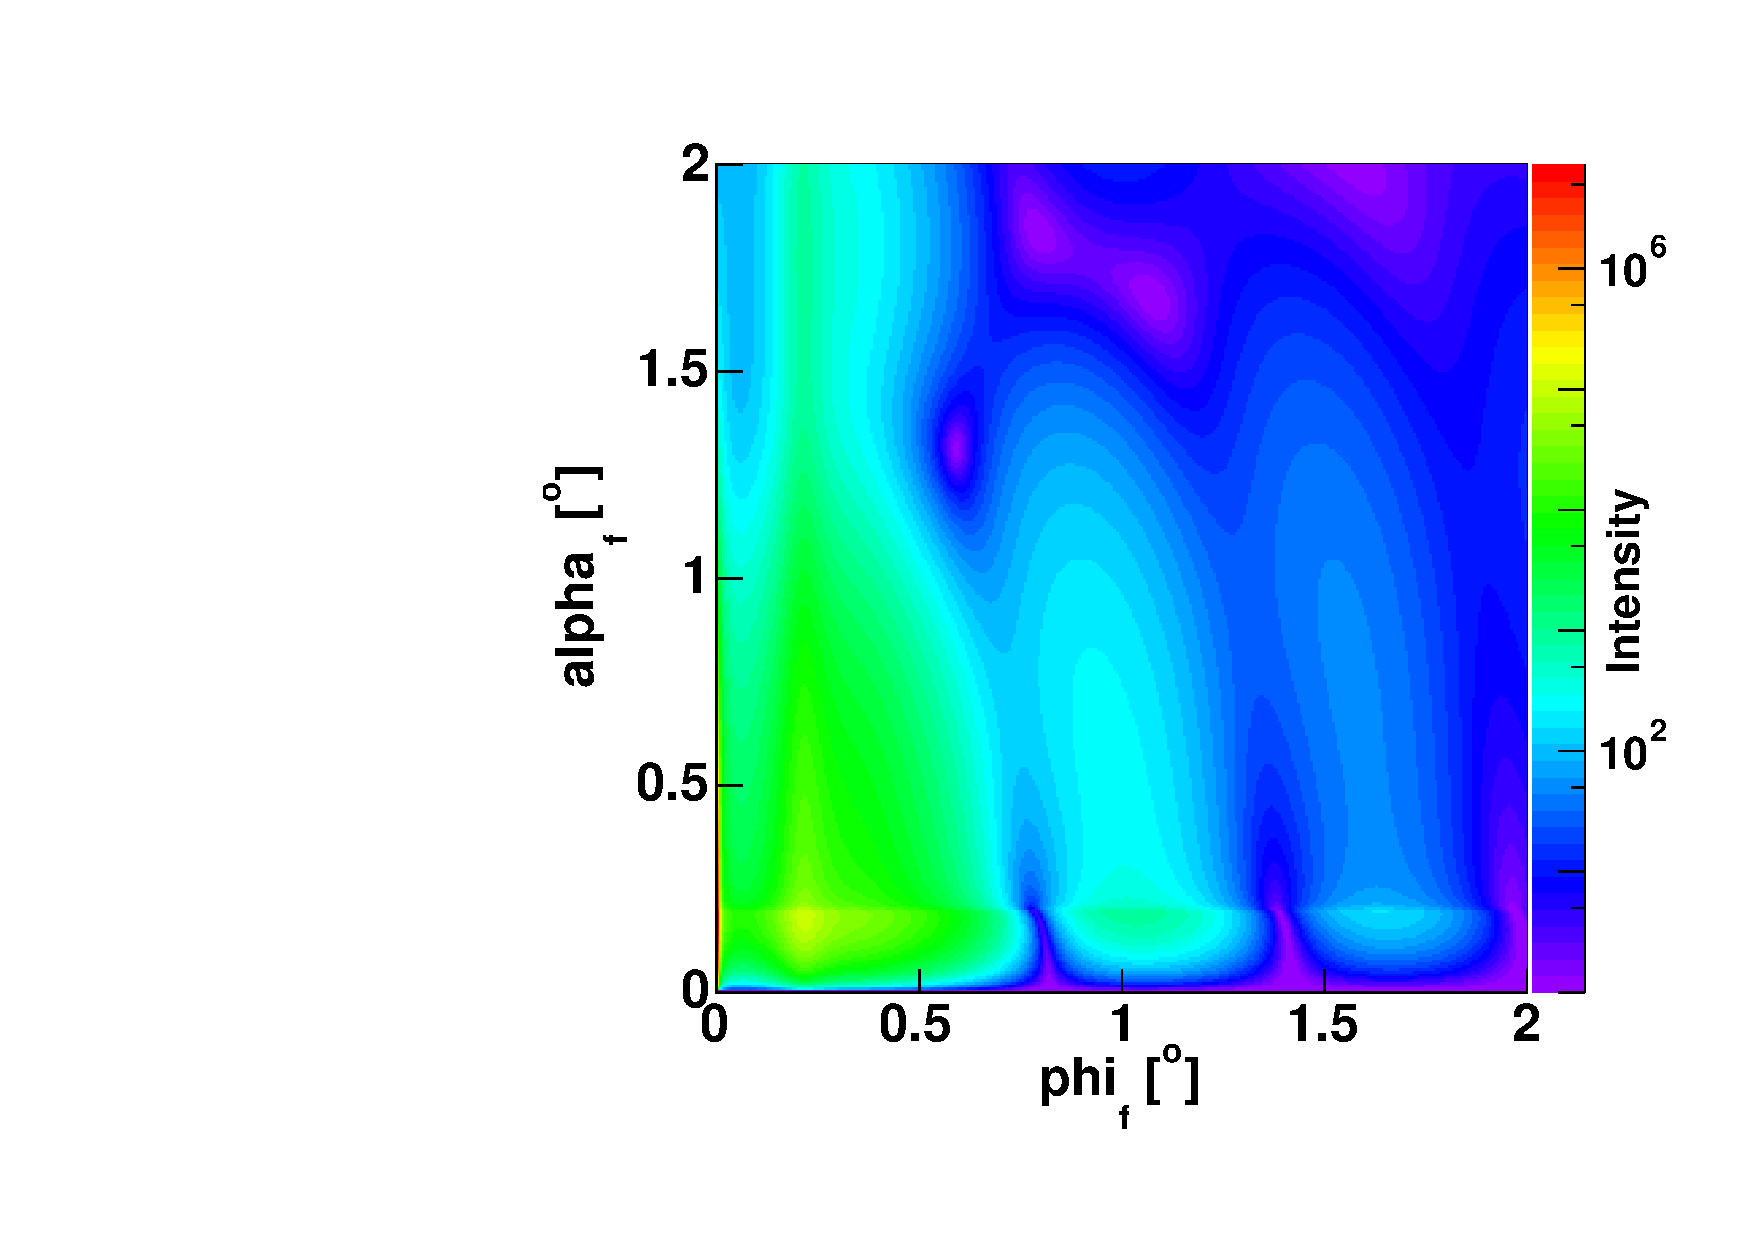
\includegraphics[angle=-90,width=0.5\textwidth]{fig/gisasmap/HSphere_1DDL.pdf}
\end{center}
\caption{Output intensity scattered from a sample made of half-spheres with the radial paracrystal interference between them. This figure has been generated using Script~\ref{lst:1dpara} for the interference function.}
\label{fig:1ddl}
\end{figure}

\FloatBarrier

\newpage
%-------------------------------------------------------------------------------
\subsection{\Code{InterferenceFunction2DLattice(L\_1, L\_2, alpha, xi)}}
%-------------------------------------------------------------------------------
where ($L_1$, $L_2$, $\alpha$, $\xi$) are shown in \cref{fig:2dlattice} with
\begin{itemize}
\item[]$L_1$, $L_2$ the lengths of the lattice cell,
\item[]$\alpha$ the angle between the lattice basis vectors $\v{a}, \v{b}$ in direct space,
\item[] $\xi$ is the angle defining the lattice orientation (set to $0$ by default); it is taken as the angle between the $\v{a}$ vector of the lattice basis and the $\v{x}$ axis of the reference Cartesian frame (as shown in \cref{fig:2dlattice}).
\end{itemize}

\begin{figure}[tb]
\begin{center}
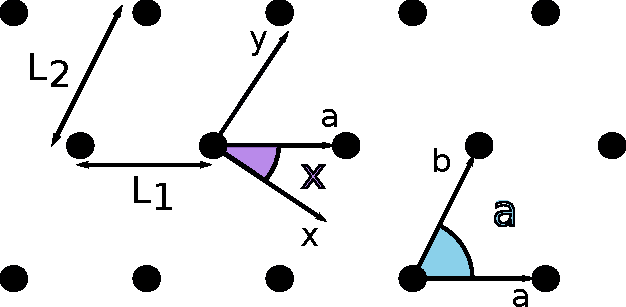
\includegraphics[width=0.5\textwidth]{fig/drawing/2Dlattice.pdf}
\end{center}
\caption{Schematic representation of a 2D lattice (top view). Such a lattice is characterized by lattice lengths $L_1$, $L_2$ and angles $\alpha$ and $\xi$.}
\label{fig:2dlattice}
\end{figure}

Like for the one-dimensional case, a probability distribution function \Code{pdf} has to be defined. One can choose between those listed in \cref{baftd} and implements it using \Code{setProbabilityDistribution(pdf)}.

\paragraph{Example} The sample used to run the simulation is made of half-spheres deposited on a substrate. The interference function is "2Dlattice" and the particles are located at the nodes of a square lattice with $L_1=L_2=20$~nm, $\v{a}\equiv \v{b}$ and the probability distribution function is Gaussian. We also use the Decoupling Approximation.

\begin{lstlisting}[language=python, style=eclipseboxed,numbers=none,nolol,caption={\Code{Python} script to define a 2DLattice interference function between hemi-spherical particles as well as the Decoupling Approximation in \Code{getSimulation()}.  The part specific to the interferences is marked in a red italic font.},label={lst:2dlatticeinterf}]
    #collection of particles
    sphere_ff = FormFactorTruncatedSphere(5*nanometer, 5*nanometer)
    sphere = Particle(m_particle, sphere_ff)
    |interference = InterferenceFunction2DLattice(20.0*nanometer, 20.0*nanometer, 90.0*degree, 0.0*degree)|
    |pdf = FTDistribution2DGauss(200.0*nanometer/2.0/M_PI, 75.0*nanometer/2.0/M_PI)|
    |interference.setProbabilityDistribution(pdf)|
    particle_layout = ParticleLayout()
    particle_layout.addParticle(sphere, 1.0)
    |particle_layout.addInterferenceFunction(interference)|

    # interference approx chosen between: DA (default) and SSCA
    |particle_layout.setApproximation(ILayout.DA)|
\end{lstlisting}

%\begin{lstlisting}[language=python, style=eclipseboxed,numbers=none,nolol]
%def get_simulation():
%    """
%    Create and return GISAXS simulation with beam and detector
%    """
%    simulation = Simulation()
%    simulation.setDetectorParameters(100, 0.0*degree, 2.0*degree, 100, 0.0*degree, 2.0*degree, True)
%    simulation.setBeamParameters(1.0*angstrom, 0.2*degree, 0.0*degree)
%    return simulation
%\end{lstlisting}


\begin{figure}[tb]
\begin{center}
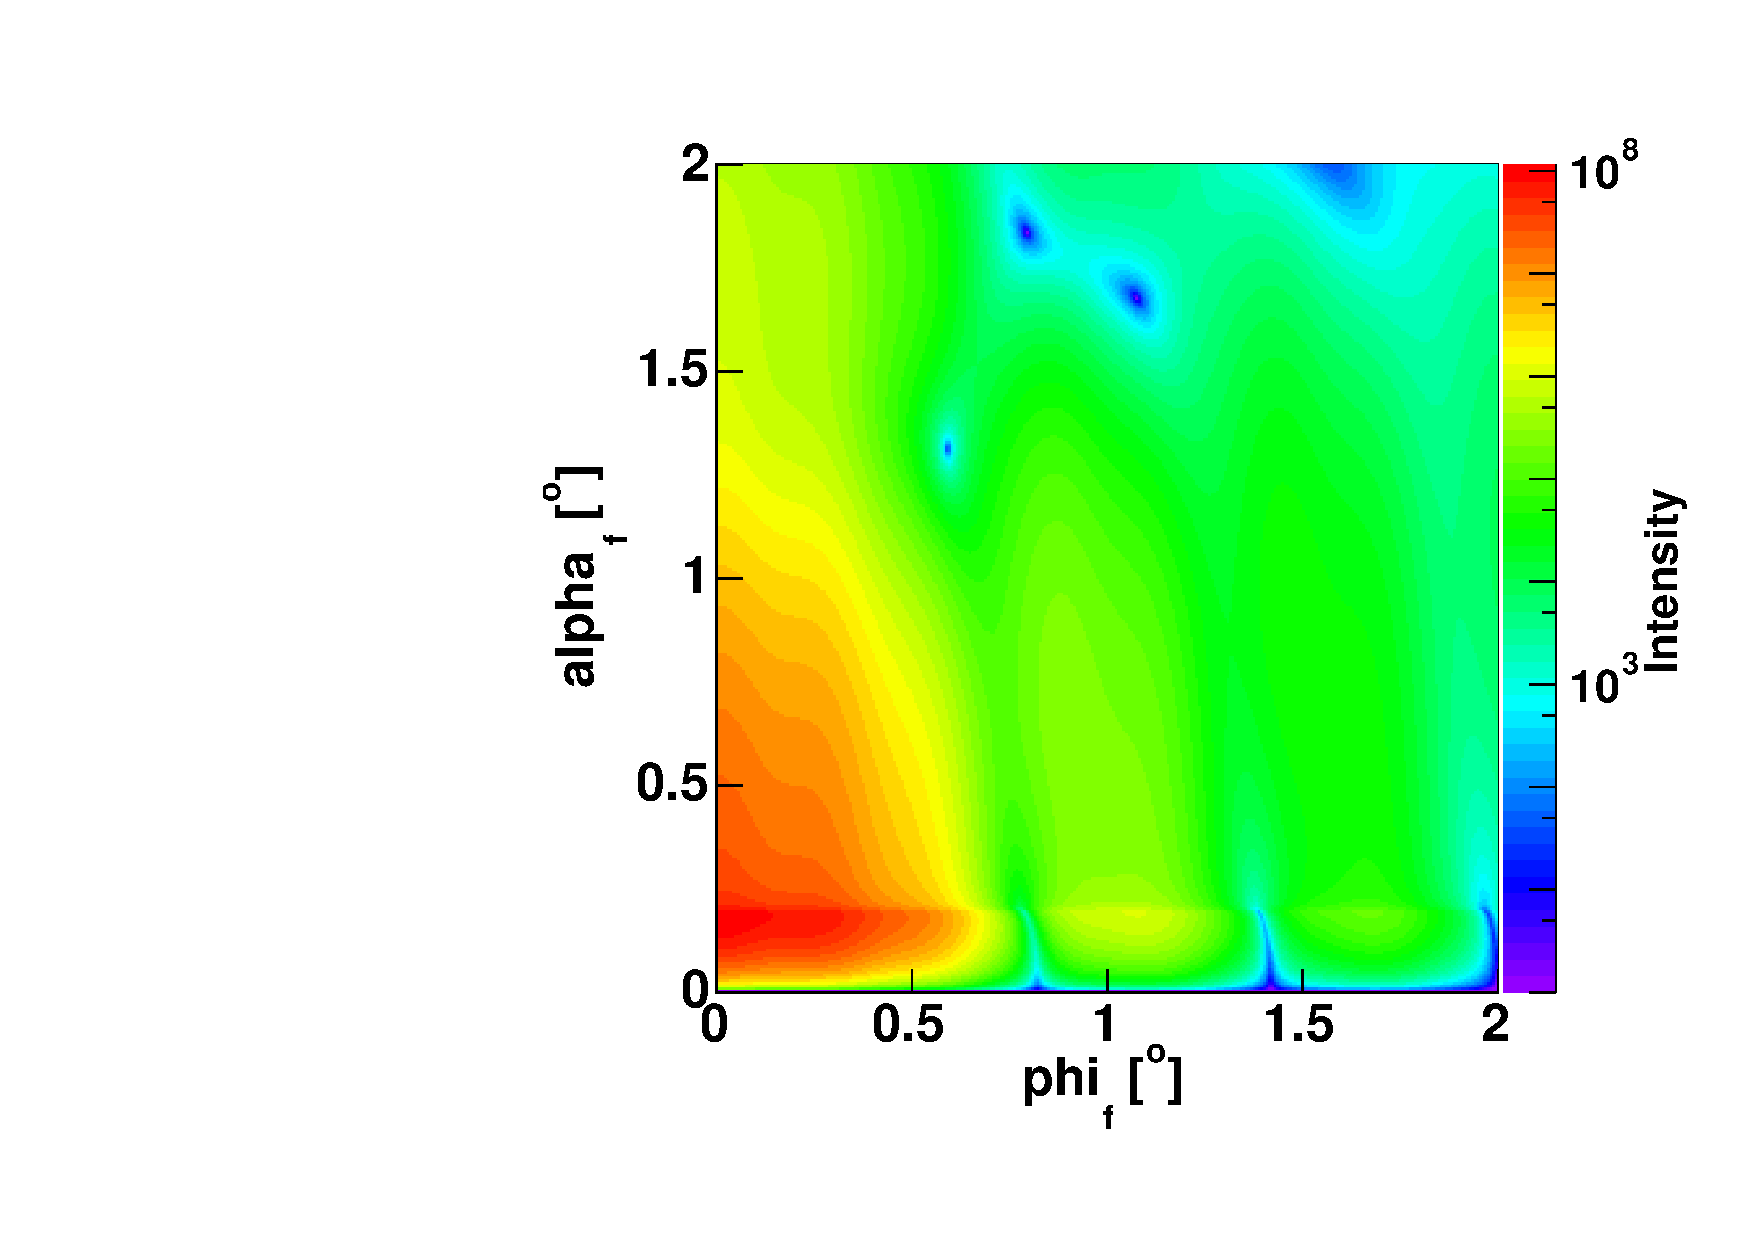
\includegraphics[angle=-90,width=0.5\textwidth]{fig/gisasmap/HSphere_2Dlattice.pdf}
\end{center}
\caption{Output intensity scattered from a sample made of half-spheres with 2DLattice interference function in the Decoupling Approximation.}
\label{fig:2dlatticeintensity}
\end{figure}

\FloatBarrier

\newpage%{\cleardoublepage}
%-------------------------------------------------------------------------------
\subsection{InterferenceFunction2DParaCrystal($L_1$, $L_2$, lattice\_angle, $xi$, damping\_length)} % TODO RESTORE \Code{}, \xi
%-------------------------------------------------------------------------------
\begin{itemize}
\item[where] $L_1$, $L_2$ are the lengths of the lattice cell,
\item[] lattice\_angle the angle between the lattice basis vectors $\v{a}, \v{b}$ in direct space,
\item[] $\xi$ is the angle defining the lattice orientation (set to $0$ by default).
\item[] \Code{damping\_length} is used to introduce finite size effects by applying a multiplicative coefficient equal to  $\exp$(-\Code{peak\_distance/damping\_length}) to the Fourier transform of the probability densities. \Code{damping\_length} is equal to 0 by default and, in this case, no correction is applied.
\end{itemize}
Two predefined interference functions can also be used:
\begin{itemize}
\item  \Code{createSquare(peak\_distance, damping\_length, domain\_size\_1, domain\_size\_2)}\\
where the angle between the base vectors of the lattice is set to $\pi/2$,
it creates a squared lattice,
\item \Code{createHexagonal(peak\_distance, damping\_length, domain\_size\_1, domain\_size\_2)}\\
where the angle between the base vectors of the lattice is set to $2\pi/3$ ,
\end{itemize}
where
\Code{domain\_size1, 2} are the dimensions of coherent domains of the paracrystal along the main axes,\\ \Code{peak\_distance} is the same in both directions and $\v{a}\equiv \v{x}$.\\

Probability distribution functions have to be defined. As the two-dimensional paracrystal is defined from two independent one-dimensional paracrystals, we need two of these functions, using\\ \Code{setProbabilityDistributions(pdf\_1, pdf\_2)}, with \Code{pdf\_{1,2}} related to each main axis of the paracrystal (see \cref{fig:2dparaschematic}).


\begin{figure}[tb]
\begin{center}
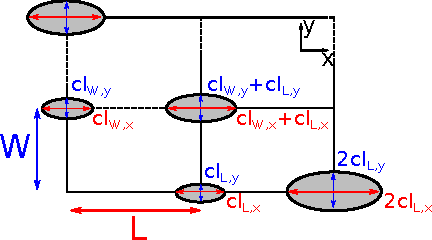
\includegraphics[width=0.75\textwidth]{fig/drawing/drawing2Dparacrystal.pdf}
\end{center}
\caption{Schematics of the ideal 2D paracrystal. The gray-shaded areas mark the regions where the probability to find a node is larger that the width at half-maximum of the distribution. $L$ and  $W$ are the mean inter-node distances along the two crystallographic axes. cl$_{(L,W),(x,y)}$ are the widths of the distribution of distance. The disorder is propagated as we add more nodes. Such a structure would be generated using \Code{InterferenceFunction2DParacrystal(L,W,90.*degrees,0,damp\_length)}, with \Code{pdf$_1$ = FTDistribution2DGauss(cl$_{L,x}$,cl$_{L,y}$)} and  \Code{pdf$_2$ = FTDistribution2DGauss(cl$_{W,x}$,cl$_{W,y}$)}.}
\label{fig:2dparaschematic}
\end{figure}


\paragraph{Example} The particles deposited on a substrate are half-spheres. The scattered beams interference via the 2DParacrystal distribution function. The paracrystal is based on a 2D hexagonal lattice with a Gaussian probability distribution function in reciprocal space.  Script~\ref{lst:2dparainterf} shows the implementation of the interference function and \cref{fig:2ddl} an example of output intensity using hemi-spherical particles.

\begin{lstlisting}[language=python, style=eclipseboxed,numbers=none,nolol,caption={\Code{Python} script to define a "2DParacrystal" interference function between particles forming an hexagonal monolayer. },label={lst:2dparainterf}]
    interference = InterferenceFunction2DParaCrystal.createHexagonal(30.0*nanometer,0.0, 40.0*micrometer, 40.0*micrometer)|
    pdf = FTDistribution2DCauchy(1.0*nanometer, 1.0*nanometer)
    interference.setProbabilityDistributions(pdf, pdf)
    particle_layout.addInterferenceFunction(interference)
\end{lstlisting}

\begin{figure}[tb]
\begin{center}
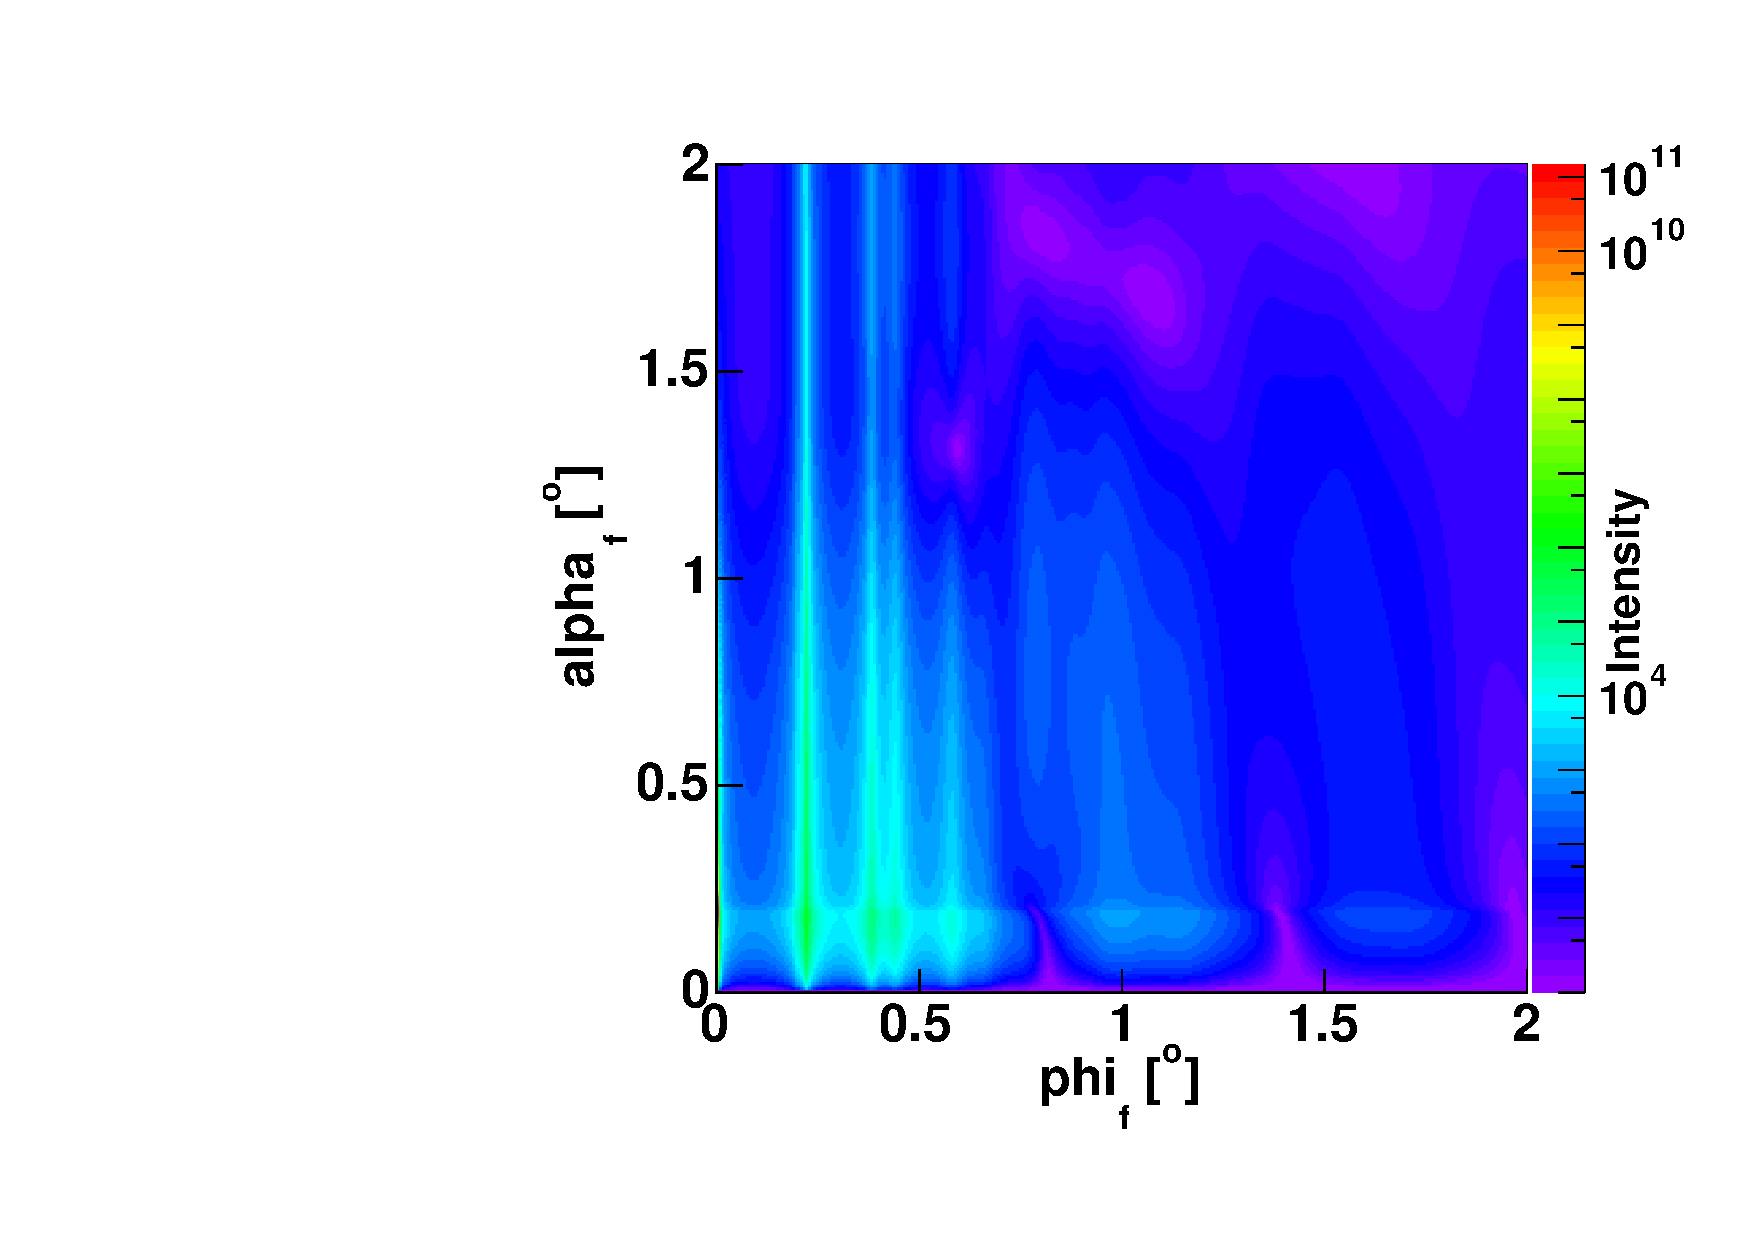
\includegraphics[angle=-90,width=0.5\textwidth]{fig/gisasmap/HSphere_2DDL.pdf}
\end{center}
\caption{Output intensity scattered from a sample made of half-spheres with 2DParacrystal interference function.}
\label{fig:2ddl}
\end{figure}

\FloatBarrier


%===============================================================================
\subsection{Summary}
%===============================================================================

\begin{table}[h]
  \footnotesize
\begin{tabular}{lll}
\hline
Function  & Parameters & Comments\\
\hline
\Code{InterferenceFunctionNone}  & None & disordered distribution \\
\hline
\Code{InterferenceFunction1DLattice} & \Code{lattice\_length} & use only with infinitely long/wide particles \\
  & $\xi=\widehat{(\v{x},\v{a})}$ & pdf=(Cauchy, Gauss or Voigt)  to be defined\\
\hline
 \Code{InterferenceFunctionRadialParaCrystal}  & peak\_distance of pdf & pdf=(Cauchy, Gauss or Voigt) to be defined \\
& damping\_length (optional) & \\
\hline
 \Code{InterferenceFunction2DLattice}  & L\_1, L\_2: lattice lengths & pdf=(Cauchy, Gauss or Voigt) to be defined\\
                        & lattice\_angle=$\widehat{(\v{a},\v{b})}$ & \\
                                                            & $\xi =\widehat{(\v{x},\v{a})}$ & \\
\hline
\Code{InterferenceFunction2DParaCrystal}  & L\_1, L\_2: lattice lengths & 2D pdf=(Cauchy, Gauss or Voigt) to be defined \\
                          & lattice\_angle=$\widehat{(\v{a},\v{b})}$ & (1 pdf per axis) \\
& $\xi=\widehat{(\v{x},\v{a})}$ & \\
& damping\_length (optional)  &  same for both axes\\
\hline
\hline
\end{tabular}
\caption{List of interference functions implemented in \BornAgain. pdf : probability distribution function, $\v{a}, \v{b}$ are the lattice base vectors, and $\v{x}$ is the axis vector perpendicular to the detector plane.}
\end{table}

\index{Particle assemblies|)}%
%\fi

%%%%%%%%%%%%%%%%%%%%%%%%%%%%%%%%%%%%%%%%%%%%%%%%%%%%%%%%%%%%%%%%%%%%%%%%%%%%%%%%%
%%
%%   BornAgain User Manual
%%
%%   homepage:   http://www.bornagainproject.org
%%
%%   copyright:  Forschungszentrum Jülich GmbH 2015
%%
%%   license:    Creative Commons CC-BY-SA
%%   
%%   authors:    Scientific Computing Group at MLZ Garching
%%               C. Durniak, M. Ganeva, G. Pospelov, W. Van Herck, J. Wuttke
%%
%%%%%%%%%%%%%%%%%%%%%%%%%%%%%%%%%%%%%%%%%%%%%%%%%%%%%%%%%%%%%%%%%%%%%%%%%%%%%%%%


\chapter{Scattering by rough interfaces}  \label{sec:Roughness}

\MissingSection

%%%%%%%%%%%%%%%%%%%%%%%%%%%%%%%%%%%%%%%%%%%%%%%%%%%%%%%%%%%%%%%%%%%%%%%%%%%%%%%%%
%%
%%   BornAgain User Manual
%%
%%   homepage:   http://www.bornagainproject.org
%%
%%   copyright:  Forschungszentrum Jülich GmbH 2015
%%
%%   license:    Creative Commons CC-BY-SA
%%   
%%   authors:    Scientific Computing Group at MLZ Garching
%%               C. Durniak, M. Ganeva, G. Pospelov, W. Van Herck, J. Wuttke
%%
%%%%%%%%%%%%%%%%%%%%%%%%%%%%%%%%%%%%%%%%%%%%%%%%%%%%%%%%%%%%%%%%%%%%%%%%%%%%%%%%

\chapter{Polarized GISAS}  \label{SPol}

In this chapter,
we generalize our treatment of wave propagation and
grazing-incidence small-angle scattering
to X-rays and polarized neutrons.
We therefore need to study vectorial wave equations,
in contrast to the scalar theory of the previous chapter.

%===============================================================================
\section{X-ray propagation}\label{Sxray}
%===============================================================================
\index{Wave propagation!X-rays}
\index{X-rays!wave propagation}

\MissingSection


%===============================================================================
\section{Polarized neutrons}\label{Snpol}
%===============================================================================

\index{Neutrons!polarized}
\index{Polarization!neutrons}

\MissingSection


%%%%%%%%%%%%%%%%%%%%%%%%%%%%%%%%%%%%%%%%%%%%%%%%%%%%%%%%%%%%%%%%%%%%%%%%%%%%%%%%
%%
%%   BornAgain User Manual
%%
%%   homepage:   http://www.bornagainproject.org
%%
%%   copyright:  Forschungszentrum Jülich GmbH 2015
%%
%%   license:    Creative Commons CC-BY-SA
%%
%%   authors:    Scientific Computing Group at MLZ Garching
%%               C. Durniak, M. Ganeva, G. Pospelov, W. Van Herck, J. Wuttke
%%
%%%%%%%%%%%%%%%%%%%%%%%%%%%%%%%%%%%%%%%%%%%%%%%%%%%%%%%%%%%%%%%%%%%%%%%%%%%%%%%%

\chapter{Instrument simulation}  \label{SInstr}

%%%%%%%%%%%%%%%%%%%%%%%%%%%%%%%%%%%%%%%%%%%%%%%%%%%%%%%%%%%%%%%%%%%%%%%%%%%%%%%%
\section{Detector images}\label{SdetImg}
%%%%%%%%%%%%%%%%%%%%%%%%%%%%%%%%%%%%%%%%%%%%%%%%%%%%%%%%%%%%%%%%%%%%%%%%%%%%%%%%

\def\tc{\text{c}}

%-------------------------------------------------------------------------------
\begin{figure}[t]
\begin{center}
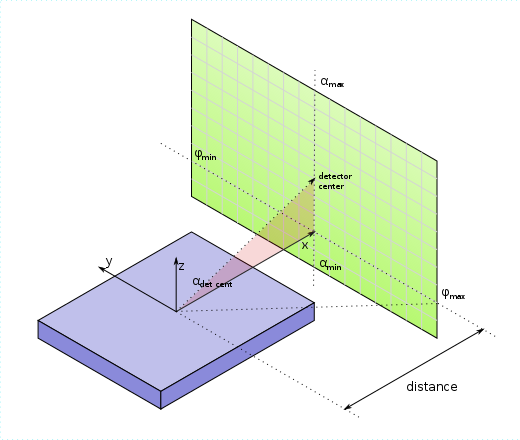
\includegraphics[width=.5\textwidth]{fig/drawing/experimental_geometry.png}
\end{center}
\caption{Experimental geometry with a two-dimensional pixel detector.}
\label{FexpGeom}
\end{figure}
%-------------------------------------------------------------------------------

To conclude this chapter on the foundations of small-angle scattering,
we shall derive the geometric factors
that allow us to convert differential cross sections into detector counts.
We shall also discuss how to present data on a physically meaningful scale.

%===============================================================================
\subsection{Pixel coordinates, scattering angles, and $\symbf{q}$ components}
%===============================================================================

We assume that scattered radiation is detected in a flat,
two-dimensional detector
that generates histograms on a rectangular grid,
consisting of $n\cdot m$ pixels of constant width and height,
as sketched in \cref{FexpGeom}.
This figure also shows the coordinate system
\index{Conventions|see {Coordinate system}}%
\index{Coordinate system}%
according to unanimous GISAS convention,
with $z$ normal to the sample plane,
and with the incident beam in the $xz$ plane.
The origin is at the center of the sample surface.
We suppose that the detector is mounted perpendicular to the $x$ axis
at a distance $L$ from the sample position.
%the $x$ axis intersects the detector plane at $(L,y_\tc,z_\tc)$.
The real-space coordinate at the center of pixel $(i,j)$ is $(L,y_i,z_i)$.
Each pixel has a width~$\Delta y$ and a height~$\Delta z$.
\index{Detector!pixel coordinate}%
\index{Pixel|see {Detector}}%

The affine-linear conversion from pixel indices $i,j$ to pixel coordinates $x_i,y_i$
requires an experimental calibration of the origin.
\Work{How is this done in \BornAgain?}
\index{Detector!calibration}%

Since the differential scattering cross section \cref{Exsectiondef}
is given with respect to a solid-angle element $\d\Omega$,
we need to express the scattered wavevector $\k_\sf$ in spherical coordinates,
using the horizontal azimuth angle~$\phi_\sf$
and the vertical glancing angle $\alpha_\sf$.
The projection of $(\alpha_\sf,\phi_\sf)$ into
the detector plane~$(y,z)$ is known as the \E{gnomonic projection}.
\index{Gnomonic projection}%
\index{Projection!wave vector to pixel coordinate}%
\index{Mapping!wave vector to pixel coordinate}%
\index{Transformation!wave vector to pixel coordinate}%
From elementary trigonometry one finds
\begin{equation}\label{Eyzdet}
  \begin{array}{lcl}
  y &=& L \tan\phi_\sf,\\
  z &=& (L/ \cos\phi_\sf) \tan\alpha_\sf.
  \end{array}
\end{equation}
\cref{Fconstalphi} shows lines of equal $\alpha_\sf$,~$\phi_\sf$
in the detector plane.
To emphasize the curvature of the constant-$\alpha_\sf$ lines,
scattering angles up to more than 25$^\circ$ are shown.
In typical SAS or GISAS,
scattering angles are much smaller,
and therefore the mapping between pixel coordinates and
scattering angles is in a good first approximation linear.
Of course \BornAgain\ is not restricted to this linear regime,
but uses the exact nonlinear mapping~\cref{Eyzdet}.

%-------------------------------------------------------------------------------
\begin{figure}[t]
\begin{center}
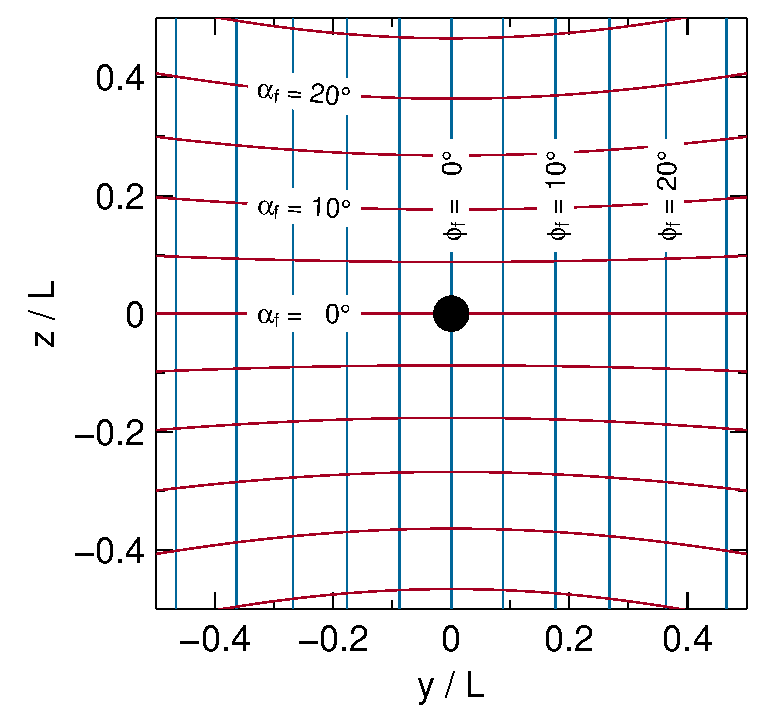
\includegraphics[width=.47\textwidth]{fig/drawing/SAS_const_alphi.ps}
\end{center}
\caption{Lines of constant $\alpha_\sf$ (red) or $\phi_\sf$ (blue)
in the detector plane,
for a planar detector at distance~$L$ from the sample.
The black dot indicates the beamstop location for
the central incident beam (SAS geometry, $\hat\k_\si = \hat x$).}
\label{Fconstalphi}
\end{figure}
%-------------------------------------------------------------------------------

To determine the scattering vector $\q_{ij}$
that corresponds to a pixel $(i,j)$,
we need to express the outgoing wavevector~$\k_\sf$ as function of $y$ and~$z$.
This can be done either by inverting \cref{Eyzdet}
and inserting the so obtained $\alpha_\sf(y,z)$ and $\phi_\sf(y)$ in
\begin{equation}\label{Ekf_by_angle}
  \k_\sf=K\left(\begin{array}{c}
   \cos\alpha_\sf\cos\phi_\sf\\
   \cos\alpha_\sf\sin\phi_\sf\\
   \sin\alpha_\sf\end{array}\right),
\end{equation}
or much more directly by using geometric similarity in Cartesian coordinates.
The result is rather simple:
\Emph{
\begin{equation}\label{Ekf_by_pixel}
  \k_\sf=\frac{K}{\sqrt{L^2+y^2+z^2}}\left(\begin{array}{c}
   L\\
   y\\
   z\end{array}\right).
\end{equation}
\vspace*{-5pt}}


%-------------------------------------------------------------------------------
\begin{figure}[t]
\begin{center}
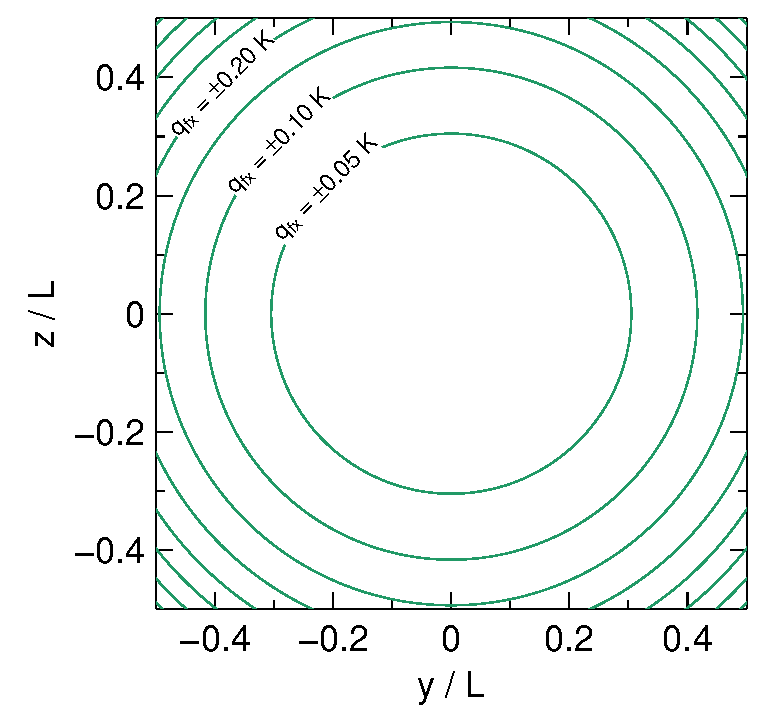
\includegraphics[width=.47\textwidth]{fig/drawing/SAS_const_q_x.ps}
\hfill
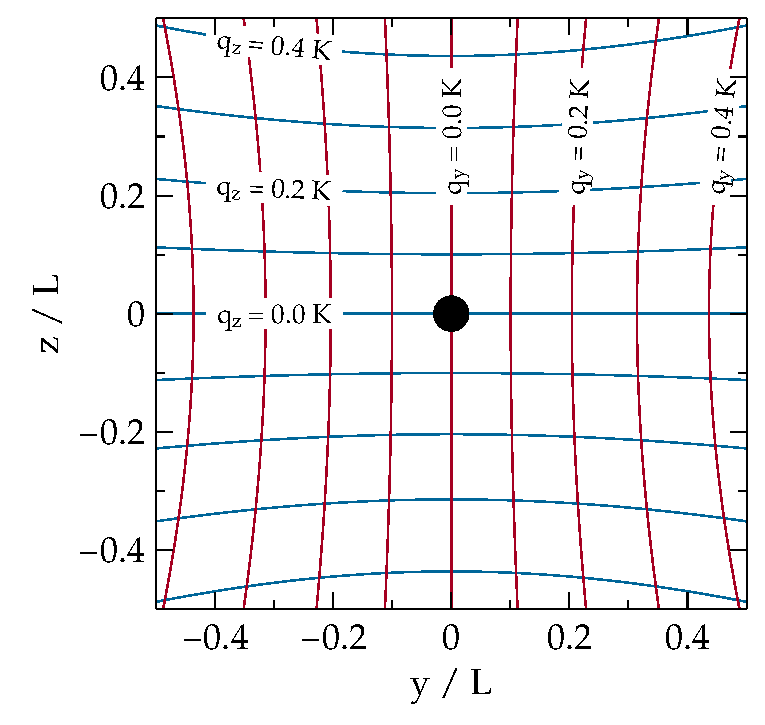
\includegraphics[width=.47\textwidth]{fig/drawing/SAS_const_q_yz.ps}
\end{center}
\caption{Lines of constant $q_x$ (left), $q_y$ or $q_z$ (right),
in units of the incident wavenumber $K=2\pi/\lambda$,
for a planar detector.
SAS geometry as in Fig.~\protect\ref{Fconstalphi}.}
\label{Fconstq}
\end{figure}
%-------------------------------------------------------------------------------

The transform \cref{Eqalgo} between pixel coordinates $y$,~$z$
and physical scattering vector components $q_y$, $q_z$
is nonlinear, due to the square-root term in the denominator of~\cref{Ekf_by_pixel}.
For $y,z\ll L$, however, nonlinear terms loose importance.

%-------------------------------------------------------------------------------
\begin{figure}[t]
\begin{center}
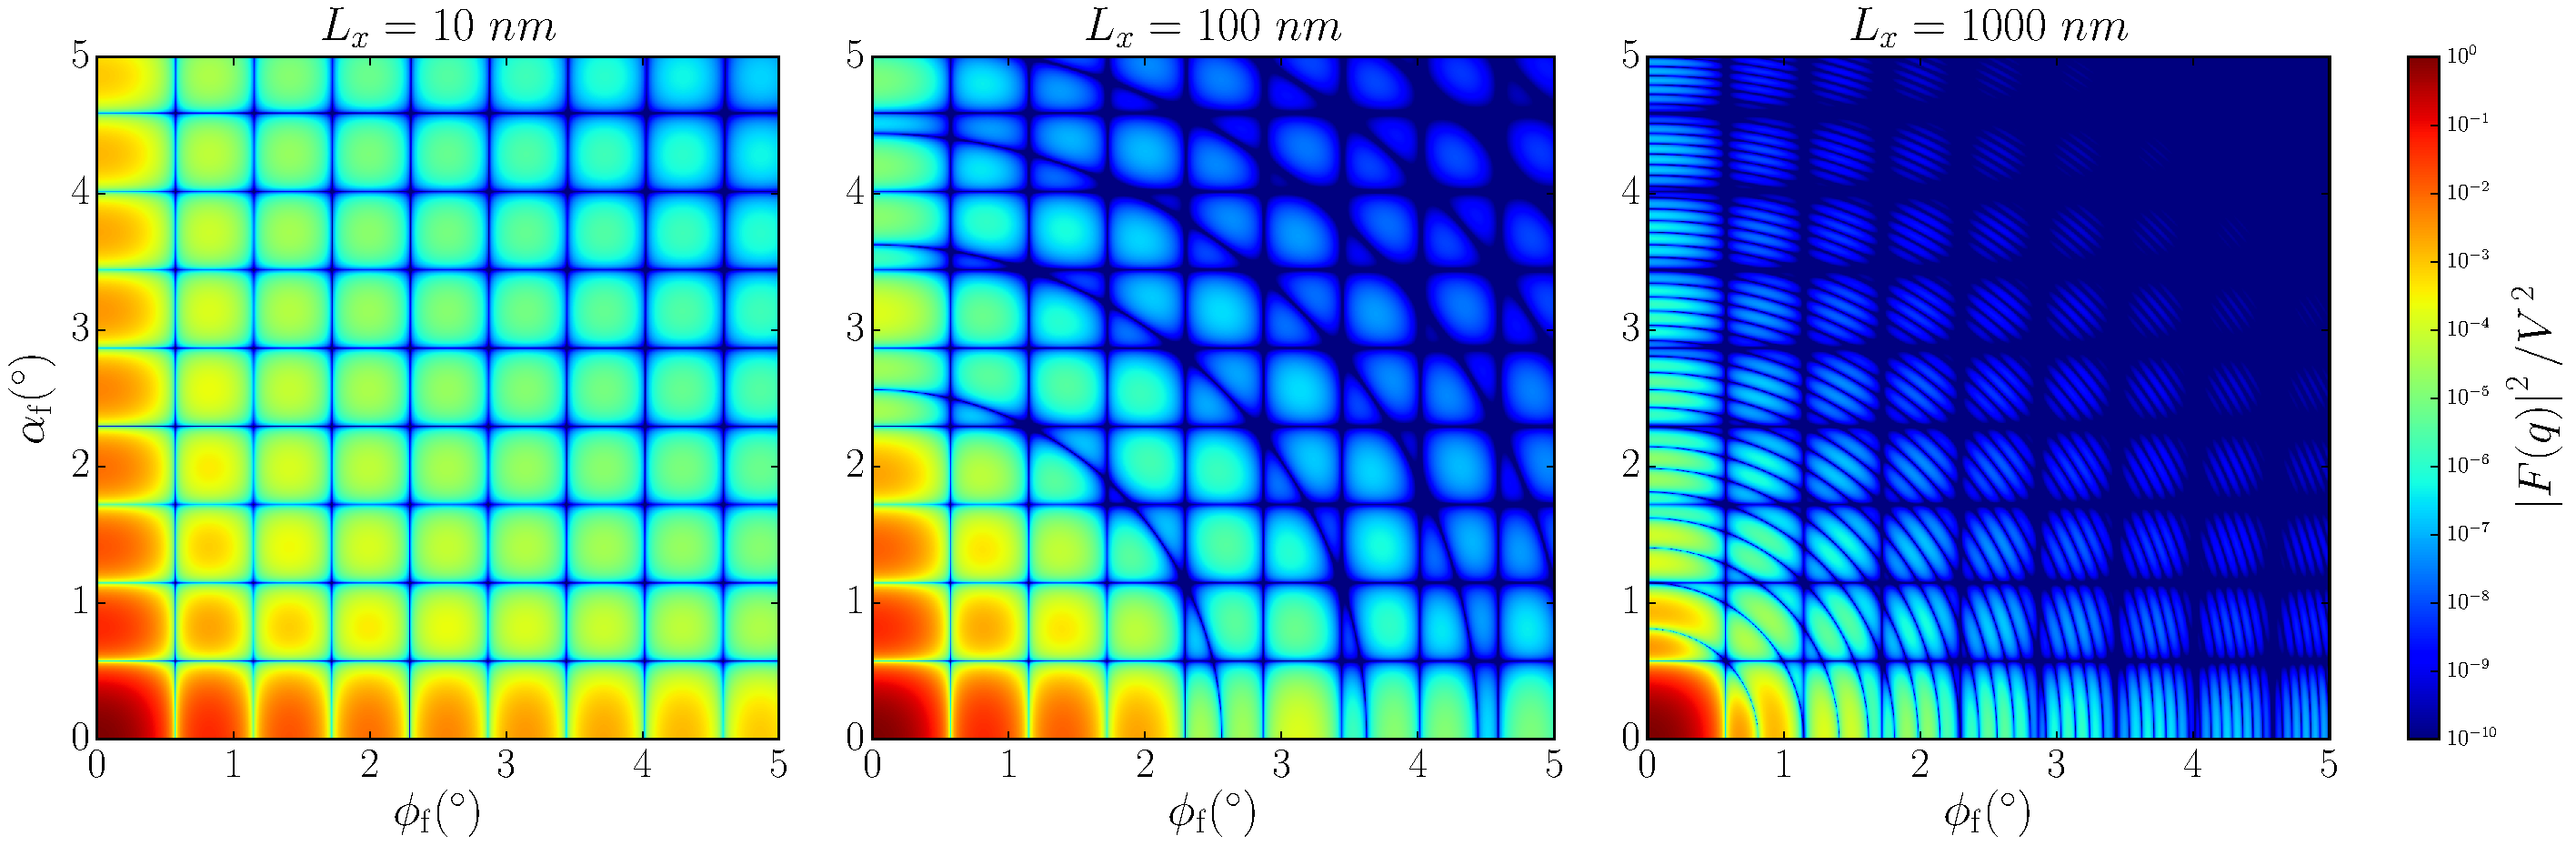
\includegraphics[width=1\textwidth]{fig/ff2/ff_det_box.pdf}
\end{center}
\caption{Simulated detector image for small-angle scattering from
uncorrelated cuboids (right rectangular prisms).
  \index{Box (form factor)}
  \index{Cuboid (form factor)}
  \index{Prism (form factor)!reactangular (Box)}
  \index{FormFactorBox@\Code{FormFactorBox}}
The incoming wavelength is 0.1~nm.
The prisms have edge lengths $L_y=L_z=10$~nm;
the length $L_x$, in beam direction, is varied as shown above the plots.
\index{Circular modulation!of detector image as function of $q_x$}
The circular modulation comes from a factor $\sinc(q_x L_x/2)$
in the cuboid form factor, with $q_x$ given by~\cref{Eqxasy}.}
\label{Fdetbox}
\end{figure}
%-------------------------------------------------------------------------------

The left detector frame in \cref{Fconstq}
shows circles of constant values of $\pm q_x$.
For given steps in $q_x$, the distance between adjacent circles
increases towards the detector center.
From \cref{Eq} and \cref{Ekf_by_pixel},
one finds asymptotically for $y,z\to L$
that $q_x$ goes with the square of the two other components of the scattering vector,
\begin{equation}\label{Eqxasy}
  \frac{q_x}{K}
  \doteq \frac{y^2+z^2}{2 L^2}
  \doteq \frac{q_y^2 + q_z^2}{2K^2}.
\end{equation}
Therefore, under typical small angle conditions $y,z\to L$
the dependence of the scattering signal on $q_x$ is unimportant:
one basically measures $v(\q)\simeq v(0,q_y,q_z)$.
The exception, for sample structures with long correlations in $x$~direction,
is illustrated in~\cref{Fdetbox}.

%-------------------------------------------------------------------------------
\begin{figure}[t]
\begin{center}
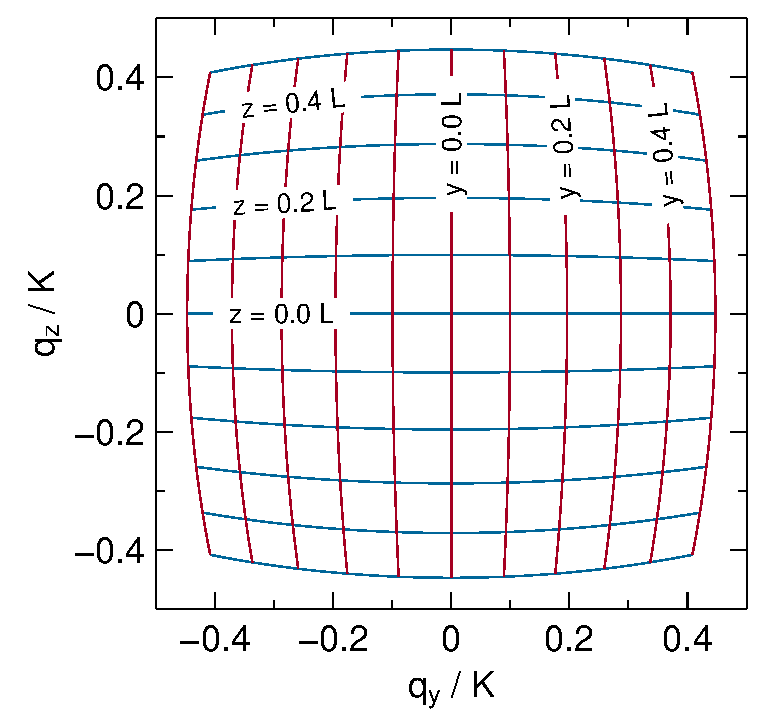
\includegraphics[width=.47\textwidth]{fig/drawing/SAS_const_p_yz.ps}
\end{center}
\caption{The outer contour of the blue and red grid
shows the border of a square detector image
after transformation into the physical coordinates $q_y$,~$q_z$.
The blue and red curves correspond to horizontal and vertical lines in the detector.}
\label{Fconstp}
\end{figure}
%-------------------------------------------------------------------------------

As anticipated in \cref{Eqxasy},
the other two components of $\q$ are in first order linear in the pixel coordinates,
\begin{equation}
  \frac{q_y}{K}=\frac{y}{L}\left(1-\frac{y^2+z^2}{2L^2}+\ldots\right),
\end{equation}
and similarly for~$q_z$.
The nonlinear correction terms lead to the pincushion distortion
shown in the right detector frame in \cref{Fconstq}.
\index{Distortion!of $q_x$, $q_y$ grid in detector plane}%
\index{Detector!distortion of $q_x$, $q_y$ grid}%
\index{Pincushion distortion}%

Since pixel coordinates are meaningful only
with respect to a specific experimental setup,
users may wish to transform detector images
towards the physical coordinates $q_y$ and~$q_z$.
As shown in \cref{Fconstp},
this would yield a barrel-shaped illuminated area
in the $q_y$,~$q_z$~plane.

To summarize this section,
the wavevector $\q_{ij}$ can be determined from the pixel indices
through the following steps:
\begin{equation}\label{Eqalgo}
  \begin{array}{cl}
      (i,j)&\\
      \downarrow&\mbox{calibrate of origin, then employ affine-linear mapping}\\
      (y,z)\\
      \downarrow&\mbox{use (\protect\ref{Ekf_by_pixel})}\\
      \k_\sf&\\
      \downarrow&\mbox{use (\protect\ref{Eq})}\\
      \q&\\
  \end{array}
\end{equation}

\Note{\indent Transforming detector images
  from pixel coordinates into the $q_y$,~$q_z$~plane is not implemented in \BornAgain,
  and not on our agenda.
  We would, however, like to hear about use cases.}

\Emph{\indent When simulating and fitting experimental data with \BornAgain,
detector images remain unchanged.
All work is done in terms of reduced pixel coordinates $y/L$ and~$z/L$.
Corrections are applied to the simulated, not to the measured data.}

\Work{\indent \ldots show how to plot $q$ grid on top of detector image \ldots}

%===============================================================================
\subsection{Intensity transformation}
%===============================================================================

The solid angle under which a detector pixel
is illuminated from the sample is in linear approximation
\begin{equation}
  \Delta\Omega
  = \cos\alpha_\sf\:\Delta\alpha_\sf\,\Delta\phi_\sf
  = \cos\alpha_\sf
    \left|\frac{\partial(\alpha_\sf,\phi_\sf)}{\partial(y,z)}\right|
    \Delta y \,\Delta z
  = \cos^3\!\alpha_\sf\, \cos^3\!\phi_\sf\: \frac{\Delta y \,\Delta z}{L^2}.
\end{equation}
\index{Detector!illumination angle correction factor}%
\index{Illumination!detector}%
Altogether,
the expected count rate in detector pixel $(i,j)$ is proportional to
\begin{equation}\label{EItrafo_cos}
  I_{ij} = \cos^3\!\alpha_\sf\, \cos^3\!\phi_\sf\:
          \frac{\partial\sigma}{\partial\Omega}(\q_{ij}),
\end{equation}
where we have omitted constant factors $L^{-2}$, $\Delta y$ and $\Delta z$.
Using pixel coordinates instead of angles, this can be rewritten as
\Emph{%
\begin{equation}\label{EItrafo_pix}
  I_{ij} = \left( 1+\frac{y^2+z^2}{L^2}\right)^{-3/2}
          \frac{\partial\sigma}{\partial\Omega}\bigl(\q_{ij}(y,z)\bigr).
\end{equation}
\vspace*{-2pt}}
%(usually as the centre between the transmitted
%and the specularly reflected beam spot).

%Tradition wants that raw data be \E{treated} or \E{reduced}
%before they are \E{analyzed}.
%In our case, raw data reduction would comprise
%the transform \cref{Eqalgo} of pixel coordinates into scattering vectors,
%and the accompanying renormalization \cref{EItrafo} of pixel counts.


%\appendix %\addtocontents{toc}{\protect\setcounter{tocdepth}{1}}
%\include{..}

\otherchapter{Bibliography}{X}
\bibliographystyle{switch}
\bibliography{jw7}

\otherchapter{List of Symbols}{Y}
\chapter*{List of Symbols}
\label{Snomencl}
\printnomenclature[6em]

\otherchapter{Index}{Z}
\small
\printindex

\end{document}
